\documentclass{article}
% Preamble for the X-regularization manuscript.
\usepackage[letterpaper, margin=1in]{geometry}
\usepackage{setspace}
\usepackage{amsmath,amssymb}
\usepackage{graphicx}
\usepackage{subcaption}
\usepackage[amsmath,thmmarks,framed]{ntheorem}
\usepackage{authblk}
\usepackage{tikz}
\usetikzlibrary{arrows.meta,calc,fit,positioning}
\usepackage{tcolorbox}
\usepackage{booktabs}
\usepackage{multirow}
\usepackage{placeins}
\usepackage{enumerate}
\usepackage{xcolor}
\definecolor{darkgreen}{rgb}{0.0,0.5,0.0}
\usepackage[colorlinks,linkcolor=red,citecolor=darkgreen,urlcolor=blue]{hyperref}
\hypersetup{
  pdftitle={Forward KL Can Be Better: Normalizing Flow Boltzmann Sampling with Log-Ratio Variation},
  pdfauthor={Qi Feng, Rongjie Lai, Di Qi, Xuda Ye}
}
\usepackage[round,authoryear]{natbib}

\usepackage[ruled,linesnumbered]{algorithm2e}
\SetKwInput{KwInput}{Input}
\SetKwInput{KwOutput}{Output}

\newtheorem{remark}{Remark}
\newtheorem{lemma}{Lemma}
\newtheorem{theorem}{Theorem}
\newenvironment{proof}{\par\medskip\noindent\textit{Proof.}\ }{\hfill$\square$\par\medskip}

\newcommand{\Le}{\leqslant}
\newcommand{\Ge}{\geqslant}
\newcommand{\D}{\mathrm{d}}
\newcommand{\KL}{\mathrm{KL}}
\newcommand{\X}{\mathrm{X}}
\newcommand{\ESS}{\mathrm{ESS}}

\theoremstyle{plain}

\newcommand{\RJ}[1]{[RJ: #1]}
\newcommand{\XY}[1]{[XY: #1]}

\title{Mode Coverage in Normalizing Flow Boltzmann Generators via Log-Ratio Variation}
\author[1]{Qi Feng}
\author[2]{Rongjie Lai}
\author[2]{Di Qi}
\author[2]{Xuda Ye}
\affil[1]{Department of Mathematics, Florida State University, Tallahassee, FL 32306}
\affil[2]{Department of Mathematics, Purdue University, West Lafayette, IN 47907}

\date{\today}
\begin{document}
\maketitle

\begin{abstract}
Normalizing flow Boltzmann generators retain a tractable pushforward density, but training with forward KL depends on target samples that may be biased or omit modes. As a result, a flow can miss target mass while its observed importance weights give a high effective sample size. We introduce the log-ratio variation $\X_\omega$, the mean absolute pairwise difference of the target-to-{pushforward} log-density ratio under a weighting measure $\omega$, and use it to define KLXX, a new loss function. Two log-ratio variations are added to the forward KL (denoted by the two X's): one weighted by the target surrogate to improve accuracy, the other by a mixture of quench and temper samples with pushforward samples to search candidate modes. We derive {\color{blue}the Fisher--Rao gradient flow of KLXX, where both variations contribute nonpositive dissipation,} and a fixed-surrogate error bound for KLXX. {\color{blue}We} use KLXX in an adaptive-staging Boltzmann generator, with exact importance reweighting and sharpening of the regularized molecular potential. We bound the sampling error of {\color{blue}its inference scheme} {\color{purple}when the stage weights are essentially bounded}, and prove it asymptotically unbiased in the sample size. From that bound we read a propagation factor that summarizes how error accumulates across stages. In the model and molecular tests, KLXX improves mode coverage and stagewise diagnostics {\color{blue}over forward KL}, and selected observables agree with independent molecular simulations. The log-ratio variations thus supply information that the forward KL loss usually omits.
\end{abstract}

% ===================== Graphical abstract =====================
\par\medskip
\noindent\makebox[\textwidth][c]{%
    \resizebox{0.9\textwidth}{!}{%
        \begingroup
        \def\KLXXEmbedded{1}%
        \ifdefined\KLXXEmbedded
    \def\KLXXBeginDocument{}
    \def\KLXXEndDocument{}
\else
\documentclass[tikz,border=5pt]{standalone}

\usepackage[T1]{fontenc}
\usepackage{lmodern}
\usepackage{amsmath,amssymb}
\usepackage{xcolor}
\usepackage{tikz}
\usetikzlibrary{arrows.meta,calc,fit,positioning}

    \def\KLXXBeginDocument{\begin{document}}
    \def\KLXXEndDocument{\end{document}}
\fi

\definecolor{ink}{HTML}{26333F}
\definecolor{line}{HTML}{7A8793}
\definecolor{neutral}{HTML}{F5F7F8}
\definecolor{target}{HTML}{3B78A7}
\definecolor{targetfill}{HTML}{EAF2F8}
\definecolor{coverage}{HTML}{C98B32}
\definecolor{coveragefill}{HTML}{FCF4E8}
\definecolor{proposal}{HTML}{4E8878}
\definecolor{proposalfill}{HTML}{EBF4F1}

\tikzset{
    >={Stealth[length=2.1mm,width=1.5mm]},
    flow/.style={->, draw=line, line width=0.85pt},
    panel/.style={
        draw=line,
        fill=white,
        rounded corners=2mm,
        line width=0.7pt,
        inner sep=2.5mm,
        align=center,
        text=ink
    },
    support/.style={panel, text width=4.75cm, minimum height=1cm},
    ratio/.style={panel, fill=neutral, text width=9.6cm, minimum height=3.55cm},
    term/.style={panel, minimum height=2.65cm, inner sep=2.2mm},
    output/.style={
        panel,
        fill=neutral,
        text width=11.4cm,
        minimum height=0.85cm,
        inner sep=1.8mm
    },
    stage/.style={
        panel,
        fill=white,
        font=\small\bfseries,
        inner xsep=4mm,
        inner ysep=1.1mm
    },
    note/.style={font=\small, text=line, fill=white, inner sep=0.5pt}
}

\KLXXBeginDocument
\begin{tikzpicture}
    % math glue is fixed, so relations in text-width nodes are not stretched
    \medmuskip=4mu \thickmuskip=5mu

    \node[font=\Large\bfseries, text=ink] at (0,5.53)
        {KLXX: one forward KL, two log-ratio variations (XX)};

    \node[output] (output) at (0,4.38) {%
        \textbf{Training aim}
        \quad $\displaystyle \nu=(G^{-1})_{\#}\pi_0\approx\pi$\\[0.5mm]
        {approximate target distribution with pushforward distribution}
    };

    \node[support, draw=target, fill=targetfill] (targetbatch) at (-5.54,2.78) {%
        \textbf{Target samples $\pi$}\\[0.8mm]
        {sequential Monte Carlo}
    };

    \node[support, draw=coverage, fill=coveragefill] (qtbatch) at (-5.54,1.08) {%
        \textbf{QT coverage $\hat\pi$}\\[0.8mm]
        {\small melt+\textbf{q}uench+\textbf{t}emper}\\[-0.2mm]
        {\small search candidate modes}
    };

    \node[support, draw=proposal, fill=proposalfill, inner ysep=1.5mm] (modelbatch) at (-5.54,-0.62) {%
        \textbf{Pushforward $\bar\nu$}\\[0.6mm]
        {\small $x\sim\pi_0\xrightarrow{\;G^{-1}\;}y\sim\nu$}\\[-0.2mm]
        {\small detached from autograd}
    };

    \node[ratio] (ratio) at (3.115,1.08) {%
    	\textbf{Pushforward density} \\[5pt]
        $\displaystyle
        \nu=(G^{-1})_{\#}\pi_0
        \quad\Longrightarrow\quad
        \nu(y)=\pi_0\bigl(G(y)\bigr)\,\lvert\det J_G(y)\rvert
        $ \\[7pt]
        \textbf{Log-ratio term} \\[5pt]
        $\displaystyle
            z(y):=\log\frac{\pi(y)}{\nu(y)}
            =U_0\bigl(G(y)\bigr)-U(y)-\log\lvert\det J_G(y)\rvert$
    };

    \draw[flow, draw=target]
        (targetbatch.east) -- ([yshift=17mm]ratio.west);
    \draw[flow, draw=coverage]
        (qtbatch.east) -- (ratio.west);
    \draw[flow, draw=proposal]
        (modelbatch.east) -- ([yshift=-17mm]ratio.west);

    \draw[flow] (output.south -| ratio.north) --
        node[right=1mm,note] {train flow $G$} (ratio.north);

    \node[stage] (losslabel) at (0,-1.45)
        {KLXX loss};
    \coordinate (ratioout) at ($(ratio.south)+(0,-3mm)$);
    \coordinate (ratioturn) at (losslabel.north |- ratioout);
    \draw[draw=line, line width=0.85pt] (ratio.south) --
        node[right=1mm,note] {evaluate $z$ on each batch} (ratioout);
    \draw[draw=line, line width=0.85pt] (ratioout) -- (ratioturn);
    \draw[flow] (ratioturn) -- (losslabel.north);

    \node[term, draw=target, fill=targetfill, text width=3.20cm]
        (meanterm) at (-6.345,-3.45) {%
        \textbf{Target mean}\\[1.2mm]
        $\displaystyle \mathbb E_{y\sim\pi}[z(y)]$\\[1.2mm]
        {\small target fit}
    };

    \node[font=\Large, text=line] at (-4.27,-3.45) {$+$};

    \node[term, draw=target, fill=targetfill, text width=3.90cm]
        (targetterm) at (-1.845,-3.45) {%
        \textbf{Target variation}\\[1.1mm]
        $\displaystyle
        \mathbb E_{y,y'\sim\pi}
        \big[|z(y)-z(y')|\big]
        $\\[1.1mm]
        {\small target regularization}
    };

    \node[font=\Large, text=line] at (0.60,-3.45) {$+$};

    \node[term, text width=6.85cm] (mixterm) at (4.52,-3.45) {%
        \textbf{Mixture variation: \textcolor{coverage}{QT}
        $+$ \textcolor{proposal}{pushforward}}\\[0.7mm]
        $\displaystyle
        \mathbb E_{y,y'\sim\xi}
        \big[|z(y)-z(y')|\big],~~ \xi=\frac{\textcolor{coverage}{\hat\pi}
        	+\textcolor{proposal}{\bar\nu}}{2}
        $\\[0.9mm]
        {\small mode coverage $\cdot$ pushforward support}
    };

    \node[fit=(meanterm)(targetterm)(mixterm), inner sep=0pt] (lossrow) {};
    \coordinate (lossbus) at ($(lossrow.north)+(0,2.2mm)$);
    \draw[draw=line, line width=0.75pt] (losslabel.south) -- (lossbus);
    \draw[draw=line, line width=0.75pt]
        (meanterm.north |- lossbus) -- (mixterm.north |- lossbus);
    \draw[flow] (meanterm.north |- lossbus) -- (meanterm.north);
    \draw[flow] (targetterm.north |- lossbus) -- (targetterm.north);
    \draw[flow] (mixterm.north |- lossbus) -- (mixterm.north);
\end{tikzpicture}
\KLXXEndDocument
%
        \endgroup
    }%
}
\par\medskip

% ===================== Section 1: Introduction =====================
\section{Introduction}
\label{sec: intro}

Sampling from a target distribution $\pi \propto \exp(-U)$ on $\mathbb R^d$ is a recurring problem in many fields including molecular simulation, Bayesian inference, and statistical physics \citep{frenkel2002understanding,robert2004monte,landau2014guide}. When $\pi$ is high-dimensional and multimodal, its mass splits among basins of $U$ separated by barriers. Local sampling kernels, including Metropolis--Hastings \citep{metropolis1953equation,hastings1970monte}, Langevin dynamics \citep{langevin1908theorie,leimkuhler2015molecular}, Nos{\'e}--Hoover dynamics \citep{nose1984unified,hoover1985canonical}, and Hamiltonian Monte Carlo \citep{duane1987hybrid}, evolve from the initial localized configuration and can therefore remain confined to one basin over accessible simulation times. When this occurs, finite-time estimates are biased toward the visited basin and give no direct account of the mass that was never reached.

Tempering and particle methods address this problem by connecting a tractable distribution to $\pi$ through intermediate distributions. Parallel tempering (PT) and replica exchange run copies of the system at several temperatures and exchange neighboring configurations, so a basin reached at high temperature can enter the low-temperature ensemble \citep{swendsen1986replica,geyer1991markov,hukushima1996exchange}. Annealed importance sampling (AIS) moves along a bridge of intermediate distributions while accumulating importance weights \citep{neal2001annealed}. Sequential Monte Carlo (SMC) uses a similar bridge but resamples and rejuvenates a weighted particle set at each level \citep{doucet2001introduction,delmoral2006sequential}. For a prescribed chemical process, umbrella sampling biases selected reaction coordinates to cross the relevant barriers and reweights the biased samples to recover a free energy profile \citep{torrie1977umbrella,kastner2011umbrella}. Nested sampling instead rewrites the normalizing integral as a one-dimensional quadrature over a likelihood threshold \citep{skilling2006nested}.

Recent work improves PT through three distinct mechanisms. Nonreversible swap schedules and tuned temperature grids accelerate round trips \citep{syed2022nonreversible}; variational-reference methods adapt the reference endpoint and its connecting path \citep{surjanovic2022variational}; and neural transports improve communication between adjacent distributions with limited overlap \citep{zhang2025accelerated}. Replica exchange has also been scaled beyond molecular simulation to stochastic-gradient samplers: replica exchange Langevin diffusion accelerates nonconvex optimization \citep{chen2019accelerating,dong2021replica}, its stochastic-gradient variant corrects the swap test for noisy energy estimates \citep{deng2020nonconvex}, and later variants reduce estimator variance to restore swap rates \citep{deng2021variance}. These accelerations strengthen communication between neighboring distributions and can transmit a discovered basin efficiently, but two inherent limits remain: a basin that no chain has visited cannot enter the target ensemble \citep{woodard2009conditions,chehab2024provable}, and the mass of a visited basin is still estimated through occupation frequencies rather than reweighting.
A more universal strategy is to learn a global transport from an easily sampled reference to the target, thereby generating independent, nonlocal proposals.

Boltzmann generators sample the target distribution with a learned transport map \citep{noe2019boltzmann}, dropping the long-time Monte Carlo iterations entirely. Let $\pi_0\propto\exp(-U_0)$ be an easily sampled reference distribution, usually Gaussian; we train an invertible normalizing flow $G:\mathbb R^d\to\mathbb R^d$ \citep{rezende2015variational,papamakarios2017masked,kingma2018glow} to fit the target-to-source transport relation $G_{\#}\pi\approx\pi_0$. The inverse map then sends independent source draws toward the target, and their pushforward distribution is $\nu:=(G^{-1})_{\#}\pi_0$. Its density is
\begin{equation}
    \nu(y)=\pi_0(G(y))\left|\det J_G(y)\right|,
    \label{eq: pushforward-density}
\end{equation}
where $J_G(y)$ is the Jacobian matrix of $G$ at $y$. The importance weight $w(y):=\pi(y)/\nu(y)$ is the ratio of the target density to the pushforward density. Reweighting by $w$ makes estimates from pushforward samples \emph{unbiased}, even when the flow is not perfectly trained. Throughout the paper we also use the \emph{log-ratio}:
\begin{equation}
	z(y) := \log w(y) = \log \frac{\pi(y)}{\nu(y)} =  U_0(G(y)) - U(y) - \log|\det J_G(y)| + \mathrm{const},
	\label{eq: log-ratio}
\end{equation}
where the constant comes from the two normalizers independent of both $y$ and $G$. The same weights define the effective sample size (ESS), a diagnostic of density agreement on the support reached by $\nu$ \citep{liu2001monte,doucet2001introduction,martino2017rethinking}. A high ESS guarantees accuracy in the flow's reached regions, but not full mode coverage of the potential $U$.


The choice of loss has a strong effect on the training quality. The original Boltzmann generator \citep{noe2019boltzmann} and its variational-inference predecessor \citep{rezende2015variational} minimize the reverse Kullback--Leibler (KL) divergence
\begin{equation}
    \text{(reverse)}\quad \KL(\nu\|\pi) = \int_{\mathbb R^d} \nu(y) \log \frac{\nu(y)}{\pi(y)} \D y \,= -\,\mathbb E_{y\sim\nu}\bigl[z(y)\bigr],
    \label{eq: reverse KL}
\end{equation}
which needs samples only from $\nu$ and evaluations of $U$. The empirical gradient is therefore accessible, but the divergence is mode-seeking \citep{wainwright2008graphical}: a mode absent from $\nu$ contributes no samples and hence no gradient. A flow can then collapse onto a subset of the target modes \citep{wu2020stochastic,felardos2023designing}. Existing approaches interleave Markov chain Monte Carlo (MCMC) kernels with deterministic layers, encode target symmetries in the architecture, reduce gradient variance near the optimum, or anneal from a smoother potential \citep{wu2020stochastic,kohler2020equivariant,vaitl2022gradients,schopmans2025temperature}. These changes can improve exploration, but their success still depends on whether the resulting sampler reaches each relevant mode.

The opposing loss minimizes the forward KL,
\begin{equation}
    \text{(forward)}\quad \KL(\pi\|\nu) = \int_{\mathbb R^d} \pi(y) \log \frac{\pi(y)}{\nu(y)} \D y \,= \mathbb E_{y\sim\pi}\bigl[z(y)\bigr],
    \label{eq: forward KL}
\end{equation}
which is mass-covering for exact distributions: it diverges if $\nu$ vanishes where $\pi$ has positive mass \citep{wainwright2008graphical}. Its empirical form, however, needs samples from the target distribution $\pi$. Existing work resolves this circularity in several ways. Maximum likelihood uses configurations from a reference thermodynamic state \citep{wirnsberger2020targeted}; adaptive flow samplers train on a running Markov chain and use the flow as a global proposal \citep{gabrie2022adaptive}; molecular flows can fit a molecular-dynamics trajectory \citep{klein2023equivariant}; and transferable architectures amortize coverage across related molecules \citep{klein2024transferable}. Persistent chains and coupled-target regression provide other approximations to the missing target expectation \citep{naesseth2020markovian,rehman2026regflow}. Because an empirical loss reflects only the regions represented by its sample source, the mass-covering property of the exact divergence does not prevent empirical mode omission. This tension motivates a loss that retains forward KL while using samples from more than one distribution.

The sampled forward KL leaves three distinct gaps. First, a mode absent from its target surrogate contributes no training points. If the flow also misses that mode, the observed weights can be nearly uniform on the reached support, so the ESS can be close to one even though target mass is absent; we call this a \emph{fake ESS} \citep{noe2019boltzmann,midgley2022flow}. Second, a finite or biased target surrogate distorts the sampled loss, and the fitted flow can inherit that error. Third, target samples give little information where the pushforward distribution places excess mass, allowing leakage between modes or into target-poor regions. Addressing one of these failures does not by itself resolve the other two.

\subsection{Main contributions in this work}
To address these gaps, we propose KLXX, a forward KL loss augmented by \emph{log-ratio variations}:
\begin{equation}
	\X_\omega(\pi\|\nu) = \mathbb E_{y,y'\sim \omega} \big[|z(y)-z(y')|\big] = \iint_{\mathbb R^d\times\mathbb R^d} \omega(y)\,\omega(y')
	\biggl|\log\frac{\pi(y)}{\nu(y)} - \log\frac{\pi(y')}{\nu(y')}\biggr| \D y\D y'.
	\label{eq: X}
\end{equation}
The log-ratio variation is the mean absolute pairwise difference of the log-ratio $z(y)$ in \eqref{eq: log-ratio}, with both points drawn independently from a given distribution $\omega$. {\color{blue}For a real random variable this functional is the Gini mean difference \citep{yitzhaki2003gini}; here it is taken of the log-ratio.}
The principal idea in $\X_\omega$ is that the log-ratio $z(y)$ should be almost surely zero on the support of $\omega$, while the difference allows the cancellation of the unknown normalizers.
As the name KLXX implies, two variation terms of the form \eqref{eq: X} are appended:

\textbf{Target variation}: $\X_\omega$ with $\omega = \pi$, the target distribution. It regularizes the forward KL loss at no additional cost: it reuses the target samples the forward KL already draws, and {\color{blue}its role is to improve} the accuracy, and hence the ESS, of the pushforward samples.

\textbf{Mixture variation}: $\X_\omega$ with $\omega = (\hat\pi + \bar\nu)/2$, the equal mixture of the quench and temper (QT) distribution $\hat\pi$ and the detached pushforward distribution $\bar\nu$, which is identical to $\nu$ but does not enter the differentiation graph. Here, the QT distribution $\hat\pi$ proactively searches the candidate modes of $U$ and serves as our major remedy against mode collapse. It is built in three steps:
	\begin{equation*}
		y\sim \pi_0 \longrightarrow \boxed{\small
		\begin{gathered}
			\text{melt: scatter with noise} \\
			y = y + m_e \zeta, \quad \zeta \sim \mathcal N(0,I_d)
		\end{gathered}
		} \longrightarrow \boxed{\small
		\begin{gathered}
			\text{quench: optimization} \\
			\dot y = -\nabla U(y)
		\end{gathered}
		} \longrightarrow \boxed{\small
		\begin{gathered}
			\text{temper: Langevin} \\
			\dot y = -\nabla U(y) + \sqrt{2}\dot B_t
		\end{gathered}
		} \longrightarrow y\sim \hat \pi
	\end{equation*}
Each sample $y$ from the source distribution $\pi_0$ is first scattered by Gaussian noise at a melt scale $m_e>0$, which carries it beyond the region the source covers. Gradient descent on $U$ then drives it into a local basin. A short Langevin run finally spreads the samples around that basin. A positive $m_e$ enables the QT distribution $\hat\pi$ to find candidate modes of $U$ that the source distribution $\pi_0$ does not reach. The QT distribution $\hat\pi$ is then paired with the detached pushforward distribution $\bar\nu$, in order to restrain the intermodal leakage between the modes QT has found.

The graphical abstract summarizes the forward KL, the target variation, and the mixture variation, together with the distribution each of them uses. Formally, in terms of the flow map $G$, the KLXX loss reads
\begin{align}
	\mathrm{KLXX}[G] & = \KL(\pi\|\nu) + \X_\pi(\pi\|\nu) + \X_{(\hat\pi+\bar\nu)/2}(\pi\|\nu) \notag \\
	& = \mathbb E_{y\sim\pi}\big[z(y)\big] + \mathbb E_{y,y'\sim\pi}\big[|z(y)-z(y')|\big] + \mathbb E_{y,y'\sim(\hat\pi+\bar\nu)/2}\big[|z(y)-z(y')|\big],
	\label{eq: KLXX-G}
\end{align}
where the log-ratio $z(y)$ defined in \eqref{eq: log-ratio} depends explicitly on $G$, while the detached pushforward distribution $\bar\nu$ requires $G^{-1}$ evaluations that do not enter the differentiation graph. Our contributions are as follows:


\begin{enumerate}
	\setlength{\itemsep}{0pt}
	\item We introduce a new KLXX loss \eqref{eq: KLXX-G}, whose components mix QT and pushforward distributions. Pairwise differences remove the unknown target normalizer, and the log-ratio variation retains $\nu=\pi$ as a minimizer. The target variation reuses the forward KL batch, while the mixture variation supplies candidate-mode and pushforward support information absent from that batch.

	\item We derive the Fisher--Rao gradient flow of the generalized KLXX loss under a general choice of parameters, {\color{blue}and identify the dissipation it induces: the two log-ratio variations enter as strictly negative terms unless the importance weight is already constant.} For a biased target surrogate, the two log-ratio variations improve the KL bound at the stationary distribution of the biased KLXX loss, and Theorem~\ref{thm: accuracy} exhibits that improvement under a mild condition.

	\item We demonstrate that QT can reach target basins outside the regions covered by the source and SMC samples. In the Himmelblau and Sparse tests, the two losses trained without QT miss remote wells, while both QT-based losses recover every mode; mixing QT and pushforward samples also reduces visible intermodal leakage (Figures~\ref{fig: himmelblau} and~\ref{fig: sparse}). We therefore report ESS together with coverage, since uniform weights on reached modes do not imply complete coverage.

	\item We build an adaptive-staging Boltzmann generator based on KLXX that uses only oracle access to the target potential $U(x)$ and its gradient $\nabla U(x)$, with SMC and QT generating the required samples on the fly. {\color{blue}Training keeps no replay buffer across steps and never differentiates through an MCMC transition: each step draws its own samples, and the mixture measure is detached.} We also bound the error of the sample set it returns. {\color{blue}Following the standard non-asymptotic analysis \citep{delmoral2004feynman,chopin2020introduction}, Theorem~\ref{thm: propagation} controls the error} at rate $N^{-1/2}$ for every bounded observable with a constant independent of $N$, so the scheme is asymptotically unbiased{\color{purple}, provided each stage weight is essentially bounded}. Reading that constant stagewise defines the propagation factors, which quantify how the error accumulates across the accepted stages; the experiments report the computable factor $\hat F_\Sigma$, assembled from the per-stage ESS. For molecular potentials, an additional continuation sharpens a regularized interaction core.
\end{enumerate}
In addition, we develop Python packages \texttt{jflows} and \texttt{jflows-md} for normalizing flow Boltzmann sampling with molecular potentials. With a JAX backend \citep{jax2018github}, the reported 22-atom alanine dipeptide run completes all ten accepted training stages in 72.7 minutes on one NVIDIA GeForce RTX 5090.


\subsection{Comparison to related works}
\label{subsec: loss-related}

The highlight of the KLXX loss \eqref{eq: KLXX-G} is the mixture of the QT distribution $\hat\pi$ with the detached pushforward distribution $\bar\nu$, which remedies mode collapse. The following ingredients draw on several ideas already present in normalizing flow training, and we compare them here.

The closest related loss is that of flow annealed importance sampling bootstrap (FAB) \citep{midgley2022flow}, which couples AIS and flow training but replaces the forward KL by the $\alpha$-divergence at $\alpha=2$. Its integrand is proportional to $\pi^2/\nu$, and thus the training minimizes the importance-weight variance. FAB targets $\pi^2/\nu$ with AIS and reuses those samples through a prioritized replay buffer that must be maintained across training; its MCMC transitions carry the gradient of the flow density. KLXX instead retains the forward KL and adds nonnegative log-ratio variations, so its additional cost is the QT construction and the variation evaluations under the mixture measure; it uses no replay buffer. The $2$-divergence gives the stronger tail penalty, whereas KLXX obtains its coverage information from QT.

Centered log-ratio penalties also arise in log-variance losses for learned diffusion samplers \citep{richter2024improved} and in log-dispersion regularization (LDR) losses for Boltzmann generators \citep{schopmans2026ldr}. The present construction therefore belongs to a broader family of log-ratio regularizers. The target-weighted comparison is quantitative: LDR-L1 uses the centered penalty $\mathbb E_\pi|z-\mathbb E_\pi z|$, and Jensen's inequality together with the triangle inequality gives $\mathbb E_\pi|z-\mathbb E_\pi z|\Le\X_\pi(\pi\|\nu)\Le2\mathbb E_\pi|z-\mathbb E_\pi z|$, so at the same coefficient $\KL$+$\X_\pi$ and LDR-L1 are comparable up to a factor of two. This suggests similar training performance, although the losses are not equivalent. The two design differences are that $\X_\pi$ pairs the forward KL integrand at two independent target points, which yields the double integral in \eqref{eq: X}, and that KLXX evaluates a second variation under a mixture of QT and pushforward samples rather than under fixed energy-labeled data.

A second family trains one flow per annealing step inside an SMC sweep. Annealed flow transport (AFT) \citep{arbel2021annealed} trains each flow by the KL divergence between the transported distribution and the next annealed target. That KL is estimated on the current weighted particles, which are then transported through the flow and resampled. Its continual repeated variant CRAFT \citep{matthews2022craft} repeats the training across successive sweeps instead of fitting each flow once. These are the closest prior works to the staged construction of Section~\ref{sec: boltzmann}, whose stage loss carries the same forward KL term; what KLXX adds at each stage are the two log-ratio variations, and in particular the mixture of QT and pushforward samples that a per-stage KL does not supply.

Constrained mass transport instead constrains the KL divergence and the entropy decay between intermediate distributions, which keeps their overlap high and avoids the mass teleportation that a fixed geometric schedule can produce \citep{vonklitzing2026constrained}; the adaptive stage selection of Section~\ref{sec: boltzmann} addresses the same difficulty through the SMC screen and the ESS gate. Sequential Boltzmann generators keep a single flow, fit it to biased molecular dynamics samples by forward KL, and anneal those samples toward the target at inference time by SMC \citep{tan2025sequential}; that transport acts after training, whereas the annealing of Section~\ref{subsec: annealing} builds the target surrogate during it, and KLXX uses no external molecular data.

A separate family replaces the loss altogether. Energy-only methods such as iDEM alternate a sampling loop with a score- or velocity-fitting loop and a replay buffer \citep{akhound2024iterated,woo2024iefm}. Adjoint sampling learns a diffusion sampler from the energy alone by stochastic optimal control \citep{havens2025adjoint}. Controlled stochastic differential equations, denoising diffusions, and flow-matching models learn a drift or velocity rather than a bijection \citep{zhang2022path,vargas2023denoising,berner2024optimal,nusken2021solving,richter2024improved}. Annealing enters this family as well: NETS augments AIS with a learned drift \citep{albergo2024nets}, and a temperature sequence of diffusion models can be annealed at inference time \citep{akhoundsadegh2025progressive}. These stochastic transports can be more expressive than the invertible architectures used here, but their terminal density often requires per-sample ODE integration \citep{he2025notrick}. We retain a bijection because the exact pushforward density, importance ratio, ESS, and reweighting are central to every term of \eqref{eq: KLXX-G} and to the final estimator. Table~\ref{tab: loss-methods} summarizes these distinctions.

A further family keeps an exact likelihood but drops the bijection. Autoregressive Boltzmann generators (ArBG) factorize the density as $p(x)=\prod_j p(x_j\mid x_{<j})$, so the likelihood needs neither a Jacobian determinant nor an ODE solve, and no map is inverted \citep{rehman2026autoregressive}. They are trained by likelihood on molecular dynamics data, whereas the generator of Section~\ref{sec: boltzmann} uses no external samples.

\begin{table}[htb]
\centering
{\small
\begin{tabular}{@{}lll@{}}
\toprule
method & loss & training mechanism \\
\midrule
reverse KL & $\KL(\nu\|\pi)$ & pushforward samples; no target sampler \\
forward KL & $\KL(\pi\|\nu)$ & annealed target surrogate in this work \\
FAB & $2$-divergence ($\pi^2/\nu$) & AIS on $\pi^2/\nu$; MCMC differentiates $\nu$; replay buffer \\
LDR & $\KL(\pi\|\nu)+\mathbb E_\pi[|z-\mathbb E_\pi z|^p]$ & fixed energy-labeled data; no extra pushforward samples \\
AFT, CRAFT & $\KL$ per annealing step & one flow per step, trained on the weighted particles \\
iDEM & energy matching & iterative sampler; stochastic transport; replay buffer \\
ArBG & maximum likelihood & autoregressive model; molecular dynamics data \\
\multirow{2}{*}{KLXX} &
\multirow{2}{*}{$\KL(\pi\|\nu)$+$\X_\pi$+$\X_{(\hat\pi+\bar\nu)/2}$} &
target annealing, QT, and detached pushforward samples \\
& & no MCMC derivative of $\nu$ or replay buffer \\
\bottomrule
\end{tabular}
}
\caption{Losses and training mechanisms for the methods discussed above. Here $z=\log(\pi/\nu)$; the LDR row gives its target-weighted form with $p=1$ for LDR-L1 and $p=2$ for LDR-L2. The forward KL row uses the SMC target surrogate of this paper but may instead use external target data. The table compares how samples enter each loss; it does not assume equal computational budgets.}
\label{tab: loss-methods}
\end{table}

{\color{blue}We compare against forward KL and its log-ratio variants rather than against the methods of Section~\ref{subsec: loss-related}. Training without external data is itself a constraint: much forward KL work fits a flow to target samples produced beforehand, so a method given those samples and one given only $U$ and $\nabla U$ are solving different problems. Molecular flows are fitted to molecular dynamics trajectories \citep{klein2023equivariant,klein2024transferable}, sequential Boltzmann generators to biased molecular dynamics samples \citep{tan2025sequential}, and autoregressive Boltzmann generators by likelihood on peptide simulation datasets \citep{rehman2026autoregressive}; LDR is trained either on simulation datasets or purely variationally \citep{schopmans2026ldr}. The remaining candidates differ in what their training loop must carry. FAB estimates the $2$-divergence, which has high gradient variance when estimated from flow samples, the difficulty its annealed importance sampling and prioritized replay buffer are designed to control \citep{midgley2022flow}; both add per-step cost, and evaluating the flow density at buffer points requires the Jacobian log-determinant, and its gradient, at configurations the current proposal did not produce. An independent study reports FAB reaching comparable accuracy on peptides at roughly three times the target energy evaluations, and resolving the metastable states of its largest system only partially \citep{schopmans2025temperature}. iDEM carries a replay buffer of the same kind and learns a diffusion sampler, so no exact pushforward density is available for importance reweighting \citep{akhound2024iterated}. LDR-L1 is within a factor of two of $\KL$+$\X_\pi$ at the same coefficient, so it is already represented among the losses we run \citep{schopmans2026ldr}. We therefore restrict the comparison to forward KL and the log-ratio variations built on it, apart from FAB on the 2D targets of Section~\ref{subsec: 2d-benchmark}, and leave a matched-budget study of the other families to future work. The mixture variation is in any case not a competitor to them: it is a way of feeding known candidate modes into a loss, and it can be added to any flow-based sampler for a given target, whatever the architecture and whatever the principal loss. Section~\ref{subsec: mol-discussion} returns to this comparison with the molecular results in hand.}

%\paragraph{Organization.}
The rest of the paper is organized as follows:
Section~\ref{sec: FR} analyzes the generalized KLXX loss in Fisher--Rao geometry, deriving its gradient flow and the accuracy bound it reaches under a biased target surrogate; Appendices~\ref{sec: appendix-FR} and~\ref{sec: appendix-accuracy} give the proofs. Section~\ref{sec: training} gives the training algorithm. Section~\ref{sec: boltzmann} proposes the adaptive-staging Boltzmann generator and bounds the error of the sample set it returns; Appendix~\ref{sec: appendix-propagation} gives the proof. Sections~\ref{sec: experiments} and~\ref{sec: molecular} report the model and molecular results, respectively.  Section~\ref{sec: conclusions} gives the conclusion.

\section{Analysis of the generalized KLXX loss}
\label{sec: FR}

In this section we consider a generalized form of the KLXX loss \eqref{eq: KLXX-G}, determined by the parameters $(\lambda,\vartheta,\alpha,\beta)$. For convenience, we write the loss $\mathcal L$ as a functional of the pushforward distribution $\nu$ rather than of the flow map $G$:
\begin{align}
	\mathcal L[\nu] & =  \KL(\pi\|\nu) + \lambda\,\X_\pi(\pi\|\nu) + \vartheta\,\X_{\alpha\hat\pi+\beta\bar\nu}(\pi\|\nu) \notag \\
	& = \mathbb E_{y\sim\pi}\big[z(y)\big] +  \lambda\, \mathbb E_{y,y'\sim\pi}\big[|z(y)-z(y')|\big] + \vartheta\, \mathbb E_{y,y'\sim \alpha\hat\pi+\beta\bar\nu}\big[|z(y)-z(y')|\big],
	\label{eq: KLXX-general-nu}
\end{align}
where the parameters satisfy $\lambda,\vartheta,\alpha,\beta\Ge0$ and $\alpha+\beta=1$, so that the mixture $\xi = \alpha\hat\pi+\beta\bar\nu$ is a probability distribution on $\mathbb R^d$. Note that the log-ratio $z = \log(\pi/\nu)$ in \eqref{eq: log-ratio} carries the entire dependence on $\nu$. Throughout the paper, we use one Greek symbol ($\pi$, $\nu$, $\mu$, \emph{etc.}) to denote both a probability distribution and its density with respect to Lebesgue measure on $\mathbb R^d$ with no further confusion.

The three subsections below take the generalized loss \eqref{eq: KLXX-general-nu} in turn: a formal account of how the mixture variation contributes to mode discovery, a derivation of exponential convergence for the Fisher--Rao gradient flow, and an accuracy bound under a biased target surrogate.

\subsection{Principle of mixture variation}
\label{subsec: mixture-variation}

The mixture distribution $\xi = \alpha\hat\pi+\beta\bar\nu$ mainly relies on the QT distribution $\hat\pi$ to search the candidate modes of the potential $U$, as described in Section~\ref{sec: intro}. The QT distribution $\hat\pi$ is generated from the source distribution $\pi_0$ in three steps: for each $y\sim \pi_0$,
\begin{enumerate}
	\setlength{\itemsep}{0pt}
	\item \textbf{Melt}: scatter with Gaussian noise, $y = y+m_e\zeta$, with $\zeta\sim \mathcal N(0,I_d)$, at a melt scale $m_e>0$ that carries $y$ beyond the region the source covers;
	\item \textbf{Quench}: descend the potential, $\dot y = -\nabla U(y)$, until $y$ settles at a local minimizer of $U$, that is, at the center of whichever basin the melted particle landed in;
	\item \textbf{Temper}: run a short Langevin trajectory, $\dot y = -\nabla U(y)+\sqrt 2\,\dot B_t$, which spreads $y$ around that center at the target temperature.
\end{enumerate}
The three names are taken directly from industrial steelmaking, where a workpiece is melted, quenched, and then tempered in that order. {\color{blue}The same three operations appear in the energy-landscape literature: melt and quench together are basin hopping \citep{wales1997global}, and the quench is the steepest-descent map carrying a configuration to the local minimum known as its inherent structure \citep{stillinger1982hidden}.}

Only melting carries the coverage: a large $m_e>0$ allows the particles to explore the region and cover all the missing modes. Quenching then uses a local gradient descent to drive these particles into the potential basins. Tempering finally restores a spread around each center, so that $\hat\pi$ is a distribution over configurations rather than point masses at the minimizers.

We illustrate the construction on a one-dimensional example. Define the 1D Rastrigin potential
\begin{equation*}
	U(x) = \frac12x^2+4\cos(2\pi x), \qquad x\in \mathbb R,
\end{equation*}
take the source distribution $\pi_0 = \mathcal N(0,1)$ and the melt scale $m_e=2.0$, and temper for a Langevin time of $0.2$ to obtain the QT distribution $\hat\pi$. Figure~\ref{fig: 1d-qt} shows $\hat\pi$ against the target $\pi\propto\exp(-U)$.

Every mode of $\pi$ is covered by $\hat\pi$, including the outer wells the source never reaches, but the probability assigned to each differs from the target one: $\hat\pi$ weights a well by the melted mass falling into it, so its outer wells carry far more than $\pi$ gives them. This is exactly complementary to the forward KL, which is accurate where its target samples land and blind elsewhere, whereas $\hat\pi$ is inaccurate everywhere and blind nowhere. The difference form of the log-ratio variation \eqref{eq: X} is what lets $\hat\pi$ be used without corrupting the fit to $\pi$: a variation asks only that the log-ratio be flat under its weighting measure, so $\hat\pi$ enters as the points at which flatness is demanded, never as an estimate of the mass they carry.

\begin{figure}[htb]
    \centering
    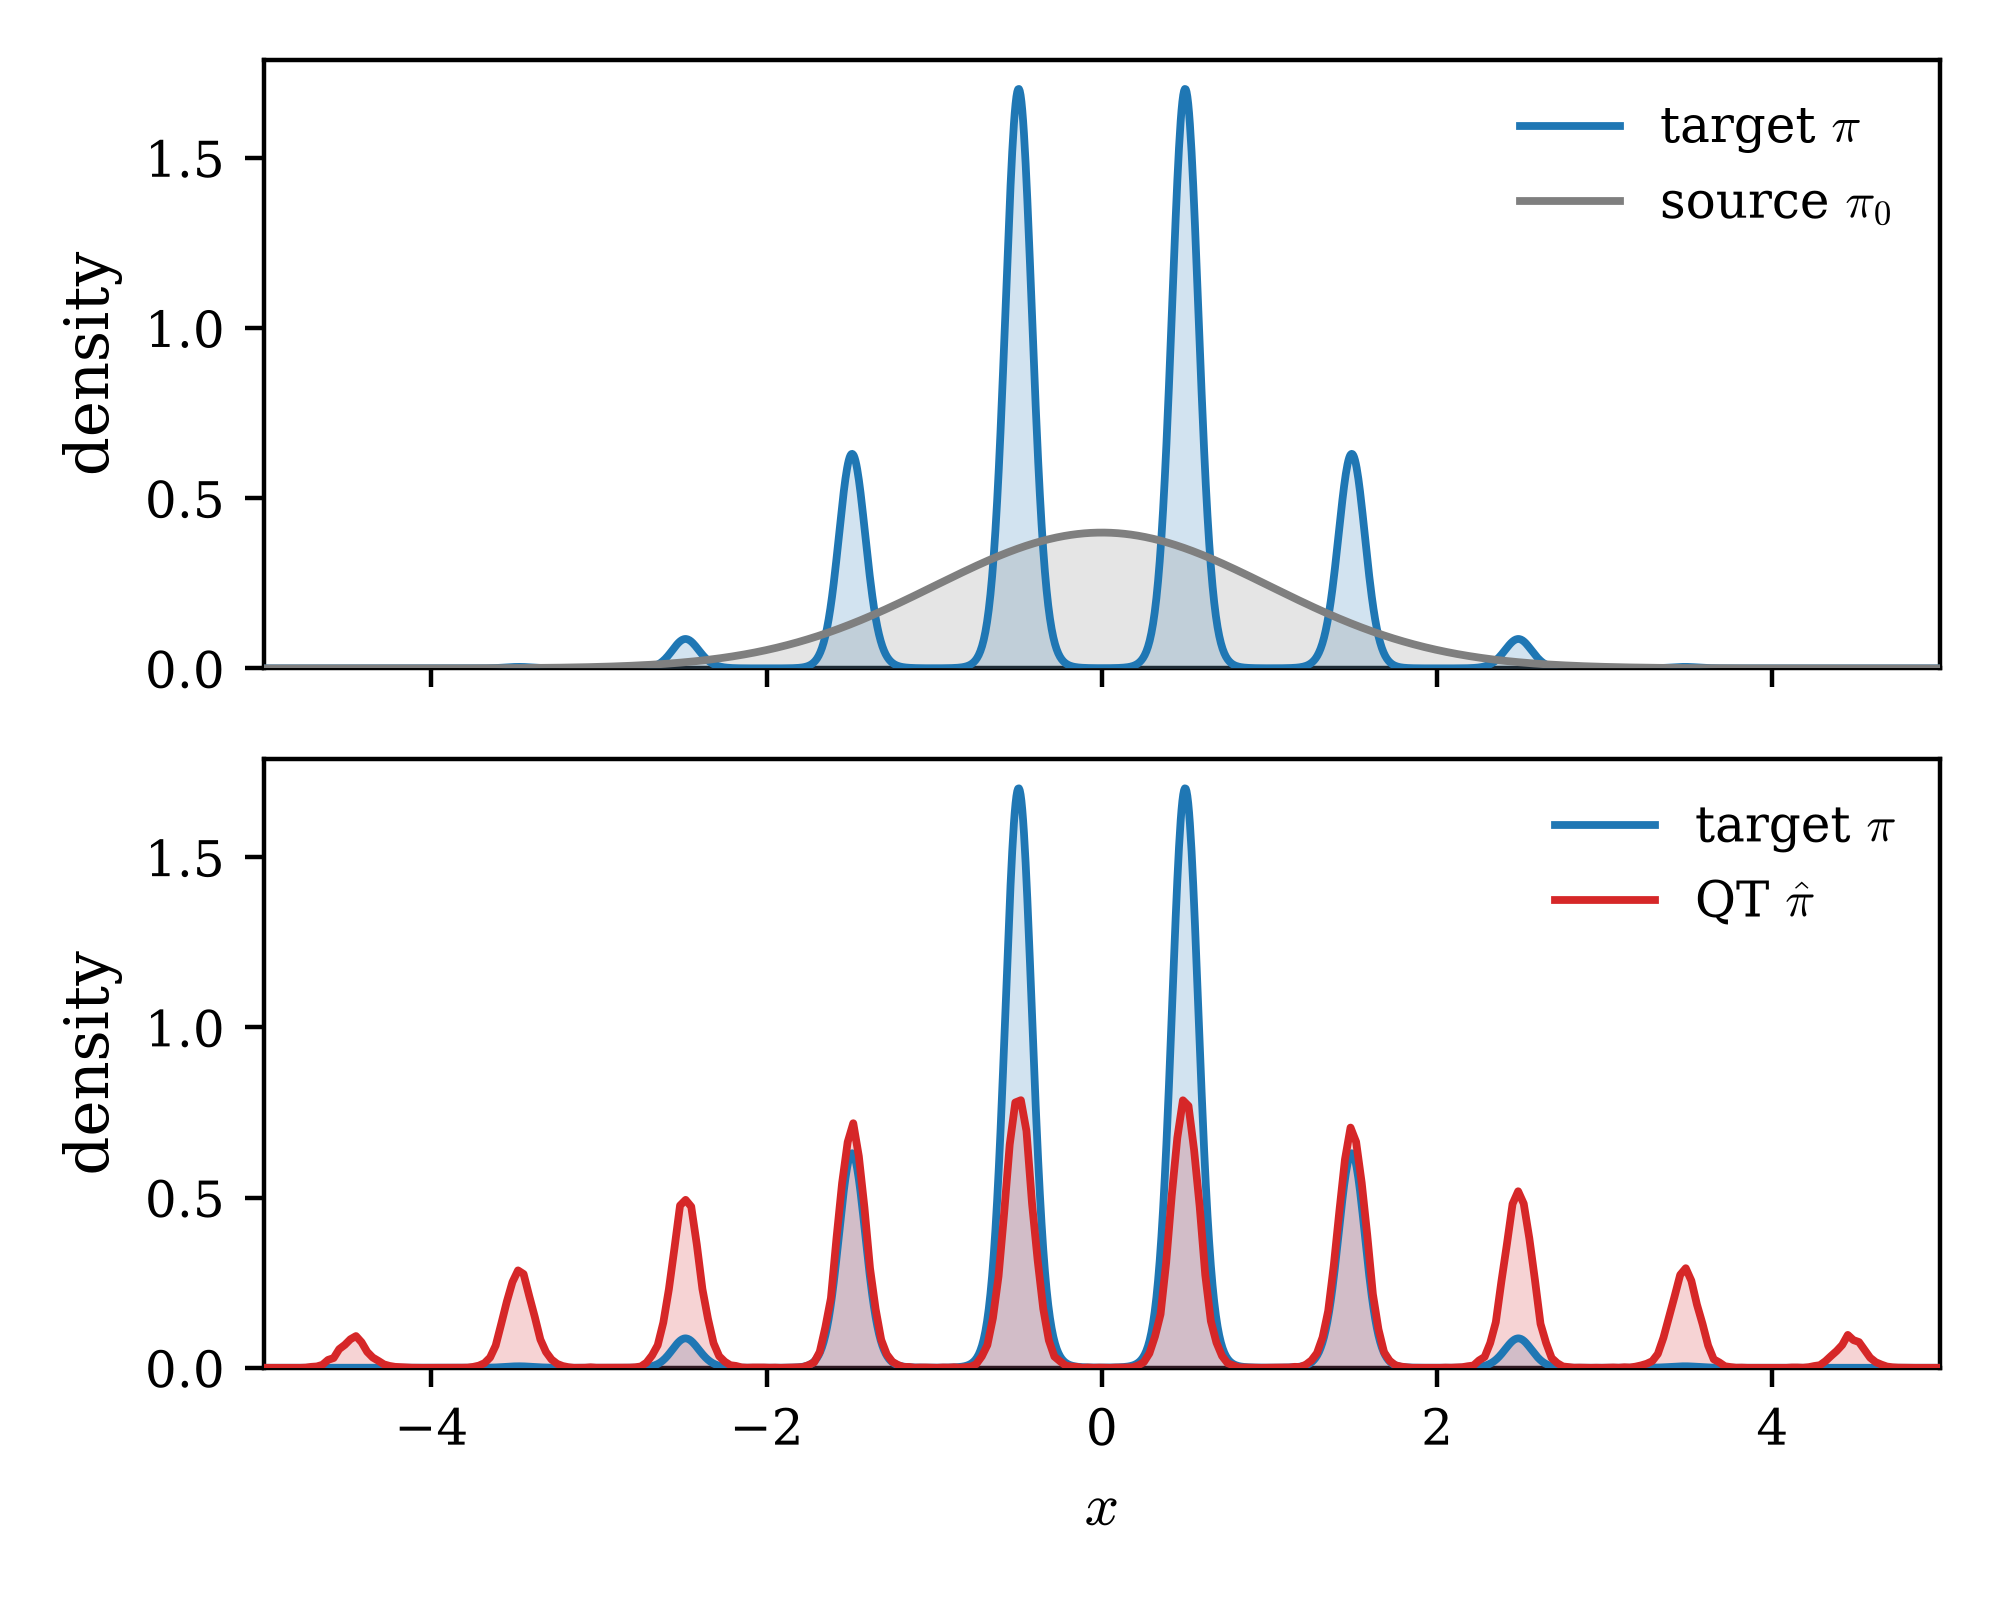
\includegraphics[width=0.55\textwidth]{figures/1d_qt_density.png}
    \caption{Quench and temper on the 1D Rastrigin target $\pi\propto\exp(-U)$ with $U(x)=\frac12x^2+4\cos(2\pi x)$. Top: the Gaussian source $\pi_0=\mathcal N(0,1)$. Bottom: the QT distribution $\hat\pi$, built from $10^5$ source samples at melt scale $m_e=2.0$ and tempered over a Langevin time of $0.2$.}
    \label{fig: 1d-qt}
\end{figure}%

However, using the QT distribution $\hat\pi$ alone in the log-ratio variation may cause \emph{intermodal leakage}: the trained flow places spurious mass between the target modes. The Sparse target shows this directly, where $\KL$+$\X_\pi$+$\X_{\hat\pi}$ recovers all four modes but leaves visible mass in the intermodal regions (Figure~\ref{fig: sparse}). The reason is that $\X_{\hat\pi}$ weights only the points $\hat\pi$ produces, and those sit in the basins of $U$; it therefore says nothing about the regions the pushforward $\nu$ occupies and $\hat\pi$ does not, which are exactly the intermodal ones. Combining it with the detached pushforward distribution $\bar\nu$ is exactly the treatment. In the log-ratio variation with the mixture distribution $\xi =\alpha\hat\pi+\beta\bar\nu$, the log-ratio $z=\log\frac{\pi}{\nu}$ is penalized to be a constant under both $\hat\pi$ and $\bar\nu$, hence during training we have approximately
\begin{equation}
	z(y) = \log\frac{\pi(y)}{\nu(y)} \approx z(y') = \log\frac{\pi(y')}{\nu(y')}, \qquad
	y\sim \hat\pi,~~y'\sim\nu.
	\label{eq: approx} 
\end{equation}
The relation \eqref{eq: approx} reflects a fundamental collision during training. On the one hand, $y$ lies in a target mode, which $\hat\pi$ supplies for every mode, and secures a large density $\pi(y)$, so $z(y)$ grows to $+\infty$ if the pushforward $\nu$ does not reach that mode. On the other hand, $y'$ lies wherever the flow sends mass and secures a positive density $\nu(y')$, so $z(y')$ decreases to $-\infty$ if the pushforward reaches the intermodal regions, where $\pi$ is negligible. Demanding that the two agree sets the divergences against each other, and the flow can satisfy both only by reaching every mode and staying out of the intermodal regions. The log-ratio variation with the mixture $\xi = \alpha\hat\pi+\beta\bar\nu$ resolves the collision: $\hat\pi$ supplies the points at which $z$ must not run high, $\bar\nu$ supplies the points at which it must not run low, and the variation balances the log-ratio across both, thus reducing the intermodal leakage.


\begin{remark}
	We do not train with the log-ratio variation alone. A variation constrains only the flatness of $z$ pointwise, while the forward KL \eqref{eq: forward KL} drives the flow globally: by Jensen's inequality it is nonnegative and zero only at $\nu=\pi$. Appendix~D.2 of the LDR study \citep{schopmans2026ldr} reports the analogous failure: training with LDR-L1 or LDR-L2 alone, without a KL term, produces qualitatively incorrect distributions.
\end{remark}

\begin{remark}
	The melting step is a design choice: Gaussian noise suits most target distributions with Gaussian tails, which is the case considered in this paper. The Gaussian noise can be wasteful when the target concentrates near a low-dimensional manifold, since most of the scattered samples land in the ambient space. Melt and quench can then be replaced by a particle dynamics carrying a pairwise repulsion, which spreads the particles apart instead of scattering each one on its own. The repulsive term of Stein variational gradient descent \citep{liu2016stein} is of this kind, and the history-dependent bias of metadynamics \citep{laio2002escaping} serves the same purpose in molecular simulation.
\end{remark}

\subsection{{\color{blue}Fisher--Rao gradient of the KLXX loss}}
\label{subsec: FR-convergence}

For an arbitrary parameter choice $(\lambda,\vartheta,\alpha,\beta)$, the generalized KLXX loss \eqref{eq: KLXX-general-nu} attains its minimum $0$ at the exact target $\pi$, {\color{blue}so we ask what the gradient flow it induces dissipates, and how the two variations enter that dissipation.}
In the Wasserstein-2 geometry, the forward KL is not displacement convex, so the Otto--Villani and Bakry--{\'E}mery arguments used for the reverse KL do not apply \citep{otto2000generalization,bakry2014analysis}. We therefore work in the Fisher--Rao (FR) geometry, where the gradient flow has an explicit form. Assume all densities are positive and regular enough for differentiation.

Let $\omega$ be a weighting distribution that is fixed under the variation, and define the \emph{nonlocal correlation} of the importance weight
\begin{equation}
	S^{\omega}(x) := \mathbb E_{y\sim\omega}\bigl[\operatorname{sgn}\bigl(w(x)-w(y)\bigr)\bigr] \in [-1,1],
	\label{eq: FR-S}
\end{equation}
which reports where $w(x)$ sits among the weights $\omega$ carries. Here $\operatorname{sgn}(\cdot)\in\{0,\pm1\}$ is the sign of a real number.
The same definition applies to the target distribution $\pi$ and to the mixture distribution $\xi=\alpha\hat\pi+\beta\bar\nu$, written as $S^{\pi}$ and $S^{\xi}$.

The FR gradient flow of the generalized KLXX loss \eqref{eq: KLXX-general-nu} is a differential equation for a time-dependent pushforward density $\nu_t$, satisfying
\begin{equation}
	\partial_t\nu_t(x) = -\,\mathrm{grad}^{\mathrm{FR}}\mathcal L(\nu_t) = \pi(x)-\nu_t(x) + 2\lambda\,\pi(x)S^{\pi}_t(x) + 2\vartheta\,\xi(x)S^{\xi}_t(x),
	\label{eq: FR-flow}
\end{equation}
where the nonlocal correlations are evaluated with the importance weight $w_t=\pi/\nu_t$,
\begin{equation}
	S^{\pi}_t(x) = \mathbb E_{y\sim\pi}\bigl[\operatorname{sgn}\bigl(w_t(x)-w_t(y)\bigr)\bigr],
	\qquad
	S^{\xi}_t(x) = \mathbb E_{y\sim\xi}\bigl[\operatorname{sgn}\bigl(w_t(x)-w_t(y)\bigr)\bigr].
	\label{eq: FR-S-t}
\end{equation}
{\color{blue}Since $\bar\nu$ is detached, $\xi=\alpha\hat\pi+\beta\bar\nu$ is held fixed when the gradient is taken and then follows $\nu_t$ along the flow. For $\beta>0$, \eqref{eq: FR-flow} is therefore not the gradient flow of one fixed functional; the dissipation identity \eqref{eq: combined-rate} below holds for it as stated.}
The mixture $\xi=\alpha\hat\pi+\beta\bar\nu$ depends on $\nu_t$ through $\bar\nu$, but $\bar\nu$ is detached and takes no part in the gradient calculation, so $\xi$ is held fixed when the variation is taken. Differentiating $\KL(\pi\|\nu_t)$ along \eqref{eq: FR-flow} gives the dissipation relation of the forward KL
\begin{equation}
	\frac{\D}{\D t}\KL(\pi\|\nu_t) = -\chi^2(\pi\|\nu_t)
	- \lambda\,\mathbb E_{x,y\sim\pi}\bigl[|w_t(x)-w_t(y)|\bigr]
	- \vartheta\,\mathbb E_{x,y\sim\xi}\bigl[|w_t(x)-w_t(y)|\bigr],
	\label{eq: combined-rate}
\end{equation}
where $\chi^2(\pi\|\nu):=\mathbb E_{\nu}\bigl[(w-1)^2\bigr]$ is the chi-squared divergence. {\color{blue}Identity \eqref{eq: combined-rate} is what the two variations contribute. At $\lambda=\vartheta=0$ the flow \eqref{eq: FR-flow} is the linear equation $\partial_t\nu_t=\pi-\nu_t$ and the dissipation is the single term $-\chi^2(\pi\|\nu_t)$. Since $\chi^2(\pi\|\nu_t)\Ge\KL(\pi\|\nu_t)$, discarding them leaves the decay $\KL(\pi\|\nu_t)\Le e^{-t}\KL(\pi\|\nu_0)$ that the forward KL already carries on its own; we record it only to note that the variations do not slow the flow.} Appendix~\ref{sec: appendix-FR} gives the derivation of the gradient flow \eqref{eq: FR-flow} and the proof details.

\begin{remark}
	{\color{blue}Identity \eqref{eq: combined-rate}} does not say how fast training converges. It describes a flow in density space. Training instead descends in the parameters of the flow map $G$, and that descent moves the density along a different path. The flow time $t$ is also not a step count. How far one step advances depends on the magnitude of the parameter gradient, and {\color{blue}\eqref{eq: combined-rate}} does not control it. {\color{blue}Fisher--Rao geometry works in unconstrained density space and therefore cannot see mode collapse, which is a pathology of the parametrization and of the optimizer; nothing in this section uses any property of the QT construction of Section~\ref{subsec: QT}.}
\end{remark}

\subsection{Accuracy under biased target surrogate}

In training the generalized KLXX loss \eqref{eq: KLXX-general-nu}, SMC approximates the target distribution $\pi$ (Section~\ref{subsec: annealing}), so the target surrogate is a biased distribution $\tilde\pi$. The corresponding biased loss is given by
\begin{equation}
	\tilde{\mathcal L}[\nu] = \mathbb E_{y\sim\tilde\pi}\big[z(y)\big] +  \lambda\, \mathbb E_{y,y'\sim\tilde\pi}\big[|z(y)-z(y')|\big] + \vartheta\, \mathbb E_{y,y'\sim \alpha\hat\pi+\beta\bar\nu}\big[|z(y)-z(y')|\big],
	\label{eq: KLXX-biased}
\end{equation}
where the log-ratio $z=\log(\pi/\nu)$ is still evaluated against the exact target, and only the outer measures of the first two terms are replaced  by the biased $\tilde\pi$. The mixture term carries no surrogate bias: $\xi=\alpha\hat\pi+\beta\bar\nu$ approximates nothing, $\hat\pi$ being supplied by QT and $\bar\nu$ being the detached copy of $\nu$.

Following the derivation of \eqref{eq: FR-flow} for the unbiased loss, the FR gradient of the biased KLXX loss \eqref{eq: KLXX-biased} with respect to $\nu$ has a similar form,
\begin{equation}
	\mathrm{grad}^{\mathrm{FR}}[\tilde{\mathcal L}](x) = \nu(x)-\tilde\pi(x) - 2\lambda\,\tilde\pi(x)S^{\tilde\pi}(x) - 2\vartheta\,\xi(x)S^{\xi}(x),
	\label{eq: FR-grad-biased}
\end{equation}
where $S^{\tilde\pi}$ and $S^{\xi}$ are the nonlocal correlations defined in \eqref{eq: FR-S}.
Let $\nu_\star$ be a stationary density of $\tilde {\mathcal L}$, at which the gradient \eqref{eq: FR-grad-biased} vanishes. Collecting the two $\tilde\pi$ terms gives
\begin{equation}
	\nu_\star(x) = \tilde\pi(x)\bigl(1 + 2\lambda\,S^{\tilde\pi}_\star(x)\bigr) + 2\vartheta\,\xi(x)\,S^{\xi}_\star(x),
	\label{eq: surrogate-stationary}
\end{equation}
where the correlation terms are evaluated with the importance weight $w_\star=\pi/\nu_\star$,
\begin{equation}
	S^{\tilde\pi}_\star(x) = \mathbb E_{y\sim\tilde\pi}\bigl[\operatorname{sgn}\bigl(w_\star(x)-w_\star(y)\bigr)\bigr],
	\qquad
	S^{\xi}_\star(x) = \mathbb E_{y\sim\xi}\bigl[\operatorname{sgn}\bigl(w_\star(x)-w_\star(y)\bigr)\bigr].
\end{equation}
Since $\bar\nu$ tracks $\nu$ as training updates it, \eqref{eq: surrogate-stationary} characterizes the densities that annihilate the gradient rather than the minimizers of a functional. At $\lambda=\vartheta=0$ it reduces to $\nu_\star=\tilde\pi$, whose error is $\KL(\pi\|\tilde\pi)$; the following theorem bounds how far the two log-ratio variations move that error.

\begin{theorem}
\label{thm: accuracy}
Fix the coefficients $(\lambda,\vartheta,\alpha,\beta)$ and let $\tilde\pi$ be a positive probability density. Let $\nu_\star$ be a positive density solving \eqref{eq: surrogate-stationary}, and $w_\star = \pi/\nu_\star$ be the importance weight, with $\mathbb E_{\tilde\pi}[w_\star]<\infty$ and $\mathbb E_{\xi}[w_\star]<\infty$. Then
\begin{equation}
	\KL(\pi\|\nu_\star) \Le \KL(\pi\|\tilde\pi)
	- \lambda\,\mathbb E_{x,y\sim\tilde\pi}\bigl[|w_\star(x)-w_\star(y)|\bigr]
	- \vartheta\,\mathbb E_{x,y\sim\xi}\bigl[|w_\star(x)-w_\star(y)|\bigr] .
	\label{eq: accuracy-bound}
\end{equation}
\end{theorem}
Both subtracted discrepancies are nonnegative, so the two log-ratio variations improve the error that a fixed biased surrogate leaves behind, under two different weightings of the same ratio $w_\star$.

{\color{blue}The size of that improvement is capped. Appendix~\ref{sec: appendix-accuracy} shows the two subtracted terms sum to $1-\mathbb E_{\tilde\pi}[w_\star]$, and nonnegativity forces $\mathbb E_{\tilde\pi}[w_\star]\in(0,1]$, so the subtraction is at most one whatever the coefficients and the dimension. The bound is therefore informative only when the surrogate is already close to the target. It also compares $\nu_\star$ with that one surrogate, at one choice of $(\lambda,\vartheta)$. The weight $w_\star$ depends on the coefficients, so the theorem does not rank one coefficient choice against another, nor one surrogate against another.}

{\color{blue}Theorem~\ref{thm: accuracy} holds a single $\tilde\pi$ fixed, while Algorithm~\ref{alg: training} rebuilds the target surrogate at every gradient step. The two are connected by averaging: the surrogate the flow descends against over a training run is the time average of the per-step SMC sample sets, and it is that averaged distribution that plays the role of $\tilde\pi$ in the theorem. A single step sees one draw from it; the run sees the average.}

% ===================== Sections 3-4: training + generator =====================
\section{Flow training with generalized KLXX loss}
\label{sec: training}

In this section we give the training algorithm for the generalized KLXX loss \eqref{eq: KLXX-general-nu}. Recall that the source and target distributions are $\pi_0\propto \exp(-U_0)$ and $\pi\propto \exp(-U)$, and that the flow map $G:\mathbb R^d\to\mathbb R^d$ is trained to fit the transport relation $\nu=(G^{-1})_{\#}\pi_0\approx\pi$. Hence the generalized KLXX loss in terms of $G$ reads
\begin{equation}
	\mathcal L[G] = \mathbb E_{y\sim\pi}\big[z(y)\big] +  \lambda\, \mathbb E_{y,y'\sim\pi}\big[|z(y)-z(y')|\big] + \vartheta\, \mathbb E_{y,y'\sim \alpha\hat\pi+\beta\bar\nu}\big[|z(y)-z(y')|\big],
	\label{eq: KLXX-general}
\end{equation}
where the log-ratio $z(y)$ defined in \eqref{eq: log-ratio} takes the explicit form
\begin{equation*}
	z(y) = \log\frac{\pi(y)}{\nu(y)} = U_0(G(y)) - U(y) - \log|\det J_G(y)|,
\end{equation*}
the normalizing constants being omitted, since they depend on neither $y$ nor $G$.

The training algorithm uses two parameters throughout: the sample size $N$, the size of the sample set that enters and leaves the training and carries the diagnostics; and the batch size $B$, the number of samples per gradient step.
The generalized KLXX loss \eqref{eq: KLXX-general} draws on three sample sets: one from the target distribution $\pi$, one from the QT distribution $\hat\pi$, and one from the detached pushforward distribution $\bar\nu$. The QT samples number $N$ and are constructed before training. The pushforward samples number $B$ and are drawn at each gradient step, where the target surrogate also approximates $\pi$ with a batch of $B$ samples.

The rest of the section is organized as follows. Section~\ref{subsec: training-algorithm} gives the KLXX training algorithm, which alternates between preparing samples and taking gradient steps; Sections~\ref{subsec: QT} and~\ref{subsec: annealing} then construct the QT and SMC samples it consumes; and Section~\ref{subsec: eval} gives two complementary diagnostics for the training quality.

\subsection{KLXX training algorithm}
\label{subsec: training-algorithm}

We begin from a sample set $\mathcal Y_0$ of size $N$ approximating the source distribution $\pi_0$, initialize the flow $G$ as an identity map, and run QT (Algorithm~\ref{alg: QT}) once to generate a QT sample set $\hat{\mathcal Y}$ of size $N$. Each gradient step then builds the target surrogate and mixture samples of size $B$ as follows:
\begin{enumerate}[(i)]
	\setlength{\itemsep}{0pt}
	\item Draw a random batch $\mathcal X_0\subset \mathcal Y_0$ of size $B$ and apply the pushforward to obtain $\mathcal X_{\nu} = G^{-1}(\mathcal X_0)$;
	\item Apply SMC (Algorithm~\ref{alg: annealing}) to $\mathcal X_\nu$ to obtain the target surrogate samples $\mathcal X_{\pi}$;
	\item Draw $B$ subsamples $\mathcal X_{\hat\pi}\subset \hat{\mathcal Y}$ from the QT samples, and mix $\mathcal X_{\hat\pi}$ and $\mathcal X_{\nu}$ with probabilities $\alpha$ and $\beta$ to obtain the mixture set $\mathcal X_{\xi}$;
	\item Evaluate the empirical loss on the target surrogate samples $\mathcal X_{\pi}$ and the mixture samples $\mathcal X_{\xi}$,
	\begin{equation}
	\widehat{\mathcal L}[G]=\underbrace{\widehat{\mathbb E}_{y\in\mathcal X_\pi}\bigl[z(y)\bigr]}_{\text{forward KL}} +
	\lambda\underbrace{\widehat{\mathbb E}_{y,y'\in\mathcal X_\pi}\bigl[|z(y)-z(y')|\bigr]}_{\text{target variation}}
	+\vartheta\underbrace{\widehat{\mathbb E}_{y,y'\in\mathcal X_{\xi}}\bigl[|z(y)-z(y')|\bigr]}_{\text{mixture variation}},
	\label{eq: KLXX-empirical}
	\end{equation}
	and take one gradient step on $G$, in which only $z(y) $ is differentiated.
\end{enumerate}
By convention $\mathcal X$ always has size $B$ and $\mathcal Y$ has size $N$. The sets $\mathcal Y_0$ and $\hat{\mathcal Y}$ are determined before training, and $\mathcal X_{\pi}$ and $\mathcal X_{\xi}$ are updated at each gradient step since their construction depends on $G$.
For a batch sample set $\mathcal X = \{y_1,\dots,y_B\}$, the empirical averages of $z(y)$ and $|z(y)-z(y')|$ appearing in \eqref{eq: KLXX-empirical} are defined by
\begin{equation}
	\widehat{\mathbb E}_{y\in \mathcal X} \big[z(y)\big] := \frac1B \sum_{i=1}^B z(y_i), \qquad \widehat{\mathbb E}_{y,y'\in \mathcal X} \big[|z(y)-z(y')|\big] := \frac1B\sum_{i=1}^B |z(y_i) - z(y_{\sigma(i)})|,
	\label{eq: empirical-variation}
\end{equation}
where $\sigma$ is a random permutation of $\{1,\dots,B\}$, so both variation terms carry its randomness. The target variation therefore costs no more than the forward KL, and the additional cost of KLXX comes from constructing the QT samples and evaluating the mixture variation. Algorithm~\ref{alg: training} collects steps (i)--(iv).

\begin{algorithm}[htb]
\setstretch{1.2}
\caption{KLXX training algorithm}
\label{alg: training}
\KwInput{source and QT sample sets $\mathcal Y_0,\hat{\mathcal Y}$; source and target potentials $U_0,U$; sizes $N,B$; loss coefficients $(\lambda,\vartheta,\alpha,\beta)$}
\KwOutput{trained flow map $G$}
Initialize $G$ to the identity map\;
\For{each gradient step}{
    \tcp{(i) pushforward}
    Draw a random batch $\mathcal X_0\subset\mathcal Y_0$ of size $B$ and set $\mathcal X_{\nu}\gets G^{-1}(\mathcal X_0)$\;
    \tcp{(ii) target surrogate}
    Apply SMC (Algorithm~\ref{alg: annealing}) to $\mathcal X_\nu$ to obtain $\mathcal X_{\pi}$\;
    \tcp{(iii) mixture}
    Draw $B$ subsamples $\mathcal X_{\hat\pi}\subset\hat{\mathcal Y}$, and mix $\mathcal X_{\hat\pi}$ and $\mathcal X_{\nu}$ with probabilities $\alpha$ and $\beta$ to form $\mathcal X_{\xi}$\;
    \tcp{(iv) gradient step}
    Take one gradient step on $G$ for the empirical loss
    \[
        \widehat{\mathcal L}[G]=\widehat{\mathbb E}_{y\in\mathcal X_\pi}\bigl[z(y)\bigr]
        +\lambda\,\widehat{\mathbb E}_{y,y'\in\mathcal X_\pi}\bigl[|z(y)-z(y')|\bigr]
        +\vartheta\,\widehat{\mathbb E}_{y,y'\in\mathcal X_{\xi}}\bigl[|z(y)-z(y')|\bigr],
    \]
    where the log-ratio $z(y) =  U_0(G(y)) - U(y) - \log|\det J_G(y)|$.
}
\end{algorithm}

\begin{remark}{
	When the sample set $\mathcal X_{\pi}$ of size $B$ is drawn from the target $\pi$, the variation term $\widehat{\mathbb E}_{y,y'\in \mathcal X_{\pi}} \big[|z(y)-z(y')|\big]$ has expectation $\frac{B-1}{B}\mathbb E_{y,y'\sim\pi}\big[|z(y)-z(y')|\big]$: the permutation in \eqref{eq: empirical-variation} fixes $i$ with probability $\frac1B$, and the term $|z(y_i)-z(y_{\sigma(i)})|$ then vanishes. The implementation leaves this factor uncorrected for simplicity.}
\end{remark}

\subsection{Constructing \texorpdfstring{$\hat\pi$}{pi-hat} by quench and temper}
\label{subsec: QT}

The QT distribution $\hat\pi$ is the wide-coverage measure for the target distribution $\pi$, and its melt, quench and temper construction was described in Section~\ref{subsec: mixture-variation}. In the discrete setting we implement the quench step with L-BFGS \citep{liu1989limited} and the temper step with the Metropolis-adjusted Langevin algorithm (MALA). Algorithm~\ref{alg: QT} writes the construction as the map
\begin{equation*}
    \hat{\mathcal Y} = \mathrm{QT}(\mathcal Y_0,U)
\end{equation*}
from the source samples $\mathcal Y_0=\{y_1,\dots,y_N\}$ and the target potential $U$ to the QT samples $\hat{\mathcal Y}=\{\hat y_1,\dots,\hat y_N\}$.

When the potential function $U$ is possibly singular, we prefer L-BFGS and MALA over plain gradient descent and unadjusted Langevin dynamics, which are less stable near the singularity. The QT samples can also be built from a subset of $\mathcal Y_0$, at lower cost.

\begin{remark}
	L-BFGS is a quasi-Newton method \citep{liu1989limited} and is not a discretization of the quench flow $\dot y = -\nabla U(y)$; its iterates do not follow that trajectory. The quench asks only for the local minimizer at the end of it, and in as few iterations as possible, so the better performance of L-BFGS over gradient descent is worth the departure from the flow.
\end{remark}

\begin{algorithm}[htb]
\setstretch{1.2}
\caption{QT: wide-coverage construction}
\label{alg: QT}
\KwInput{source sample set $\mathcal Y_0 = \{y_1,\dots,y_N\}$, target potential $U$, melt scale $m_e$}
\KwOutput{wide-coverage set $\hat{\mathcal Y} = \{\hat y_1,\dots,\hat y_N\}$ forming $\hat\pi$, written $\hat{\mathcal Y} = \mathrm{QT}(\mathcal Y_0,U)$}
\tcp{melt}
Scatter the samples $y_i \gets y_i + m_e\zeta_i$ with $\zeta_i \sim \mathcal N(0, I_d)$ i.i.d. and melt scale $m_e > 0$\;
\tcp{quench}
Drive each sample toward a mode center of $\pi$ by L-BFGS on $U$, updating $y_1,\dots,y_N$\;
\tcp{temper}
Spread the samples around each mode, $\hat y_{1:N} \gets \mathrm{MALA}(y_{1:N}, U)$\;
\end{algorithm}

\subsection{Approximating $\pi$ by sequential Monte Carlo}
\label{subsec: annealing}

Step (ii) of the KLXX training algorithm (Algorithm~\ref{alg: training}) builds the target surrogate samples $\mathcal X_{\pi}$ on the fly, at every gradient step, since samples from $\pi$ are not directly available. We form them by reweighting the pushforward samples $y_1,\dots,y_B$ drawn from $\nu=(G^{-1})_{\#}\pi_0$. The importance weight is
\begin{equation}
	w(y)
	= \exp\Big( U_0(G(y)) - U(y) - \log|\det J_G(y)| \Big)
	= \frac{\pi(y)}{\nu(y)},
	\qquad y \in \mathbb R^d.
	\label{eq: weight}
\end{equation}
In high dimensions, however, $\pi$ and $\nu$ can differ greatly, so the weights can collapse onto a few outliers. We therefore reweight through $M+1$ bridging distributions
\begin{equation}
	\mu_m(y) \propto \nu(y)^{1-\frac{m}{M}} \pi(y)^{\frac{m}{M}} \propto ((G^{-1})_{\#}\pi_0)(y)\, w(y)^{\frac{m}{M}}, \qquad m = 0,1,\dots,M,
	\label{eq: mu-m}
\end{equation}
so that $\mu_0 = \nu$ and $\mu_M = \pi$. Each level reweights by only $w(y)^{1/M}$, reducing the degeneracy of direct importance sampling.
After each reweighting, we resample and rejuvenate the duplicates before the next level with MALA \citep{roberts1996exponential}, which is unbiased for $\pi$.


\begin{algorithm}[htb]
	\setstretch{1.2}
	\caption{SMC for a biased target surrogate}
	\label{alg: annealing}
	\KwInput{pushforward samples $y_1,\dots,y_B$ from $\nu = (G^{-1})_{\#}\pi_0$, target distribution $\pi$, ladder length $M$}
	\KwOutput{biased target-surrogate batch $y_1,\dots,y_B$ approximating $\pi$}
	
	\For{$m = 1,\dots,M$}{
		Compute the incremental weights $w(y_i)^{1/M}=\exp(z(y_i)/M)$ on $y_1,\dots,y_B$\;
		\tcp{resample}
		Resample $y_1',\dots,y_B'$ from $y_{1:B}$ with weights $w(y_i)^{1/M}$\;
		\tcp{rejuvenate under the target}
		Diffuse the resampled duplicates by a short MALA chain on $\pi$, $y_{1:B} \gets \mathrm{MALA}(y_{1:B}', U)$\;
	}
\end{algorithm}
\medskip
\noindent
An SMC sampler that leaves every level of the path \eqref{eq: mu-m} invariant would rejuvenate at level $m$ with a Markov kernel invariant for $\mu_m$. For $m<M$, a MALA kernel for $\mu_m$ would require $\nabla_y\log\nu(y)$ and hence positional derivatives of the flow density, including $\nabla_y\log|\det J_G(y)|$; at $m=M$, this term disappears because $\mu_M=\pi$. Algorithm~\ref{alg: annealing} instead applies MALA directly under $\pi$, using only $-\nabla U$ in its proposal. MALA preserves $\pi$ but not the intermediate $\mu_m$, so the output is a biased target surrogate: the kernel needs only $-\nabla U$, at the cost of not leaving each intermediate $\mu_m$ invariant.

The SMC construction in Algorithm~\ref{alg: annealing} differs from the AIS of FAB \citep{midgley2022flow}. FAB places the flow inside the chains, and its MCMC transitions target the surrogate $\pi^2/\nu$, whose log-density gradient is
\begin{equation*}
	\nabla_y \log \frac{\pi^2(y)}{\nu(y)} = -2\nabla U(y) - \nabla_y \log\nu(y),
\end{equation*}
and therefore contains the positional gradient of the pushforward density at every MCMC step. FAB trains from a prioritized replay buffer of weighted AIS samples with a staleness correction. Reusing this buffer reduces repeated AIS generation but adds storage, prioritized sampling, and correction work. Here every MALA chain instead targets $\pi$ and uses only $-\nabla U$; the flow enters through the initial pushforward samples and evaluations of $z$. Each gradient step starts from a new source batch, so no replay buffer is kept.

The exploration costs also differ. Relative to forward KL, KLXX adds the QT construction and the pairwise log-ratio evaluations. The target variation $\X_\pi$ reuses the target batch, and the mixture term evaluates one additional batch. Coverage then comes from the fixed $N$-sample QT set of Section~\ref{subsec: QT}, whereas FAB relies on its AIS budget for exploration and on the stronger tail penalty of its $2$-divergence.

\begin{remark}
	In principle, an SMC sampler can propagate from the source $\pi_0$ to the target $\pi$ on its own, with no flow at all. That choice has two drawbacks. First, such a sampler explores only where its own trajectories go, so nothing guarantees coverage of the target modes; the QT set of Section~\ref{subsec: QT} is what supplies candidate modes in KLXX. Second, with no flow to deform the proposal toward the next distribution, each level reweights and resamples at a much lower ESS, and repeated resampling of a degenerate weight set raises the Monte Carlo error of the returned samples.
	
	The Boltzmann generator of Section~\ref{sec: boltzmann} compares each trained flow with the identity proposal and keeps whichever has the larger sample ESS, so an accepted stage is never worse than the identity in that diagnostic, up to the finite sample set. The identity proposal itself propagates by reweighting, resampling, and MALA alone. Section~\ref{sec: alkane-results} reports the corresponding experiments: the KLXX Boltzmann generator has the smallest propagation factor in all ten recorded alkane settings, while forward KL approaches the identity result as the molecule grows.
\end{remark}

\subsection{Evaluation: ESS, coverage, and importance sampling}
\label{subsec: eval}

We assess the quality of the pushforward samples through two complementary diagnostics. The ESS measures density agreement through the observed importance weights on support reached by the flow. Coverage instead checks whether the pushforward samples reach the regions represented by a fixed QT reference set. A high ESS can coexist with a missing mode, while high coverage does not establish the correct relative density within the reached regions. We therefore report the two diagnostics together.

At evaluation time the trained flow $G$ supplies the pushforward distribution $\nu=(G^{-1})_{\#}\pi_0$ and its tractable density $\nu(y)=\pi_0(G(y))|\det J_G(y)|$. The importance weight $w(y)$ in \eqref{eq: weight} can therefore be evaluated on pushforward samples without fitting another density model. Let $x_1,\dots,x_N$ be samples from the source $\pi_0$ and let $y_i = G^{-1}(x_i)$, so that $\mathcal Y=\{y_1,\dots,y_N\}$ are pushforward samples with weights $w_i=w(y_i)$.

The first diagnostic is the ESS, normalized to $(0,1]$ by dividing the classical ESS by the sample count $N$. For the importance weights $(w_1,\dots,w_N)$, define
\begin{equation}
    \ESS(w) = \frac{\big(\sum_{i=1}^{N} w_i\big)^2}{N \sum_{i=1}^{N} w_i^2} \in (0,1].
    \label{eq: ESS}
\end{equation}
The upper bound follows from Cauchy--Schwarz and is attained when all weights are equal. The factor $N$ distinguishes this normalized ESS from the classical count $(\sum_iw_i)^2/\sum_iw_i^2\in[1,N]$ \citep{martino2017rethinking}. A high ESS indicates uniform observed weights only on support reached by $\nu$; a target mode absent from the sample cannot lower it.

To detect such missing modes, we pair the ESS with the coverage diagnostic of \citet{naeem2020reliable}. Let $\hat{\mathcal Y} = \{\hat y_1,\dots,\hat y_N\}$ be the QT sample set produced by Algorithm~\ref{alg: QT}. For each $1 \Le i \Le N$, the $\kappa$-nearest-neighbor radius of $\hat y_i$ (with $\kappa = 5$) is
\begin{equation}
    \mathrm{NND}_\kappa(\hat y_i;{\hat{\mathcal Y}}) = \inf\Big\{ r \Ge 0 :
    \# \big\{1\Le j \Le N: 0 < |\hat y_i - \hat y_j| < r\big\} \Ge \kappa
    \Big\},
\end{equation}
i.e., the distance from $\hat y_i$ to its $\kappa$-th nearest neighbor in $\hat{\mathcal Y}$. The coverage of $\mathcal Y$ in $\hat{\mathcal Y}$ is then
\begin{equation}
    \mathrm{Coverage}_\kappa({\mathcal Y;\hat{\mathcal Y}}) =
    \frac{1}{N} \sum_{i=1}^{N} \mathbf 1\Bigl\{
        \exists  1\Le j\Le N : |y_j - \hat y_i| \Le \mathrm{NND}_\kappa(\hat y_i;\hat{\mathcal Y})
    \Bigr\},
\end{equation}
i.e., the fraction of points in $\hat{\mathcal Y}$ whose $\kappa$-nearest-neighbor ball contains a point of $\mathcal Y$. A coverage close to $1$ indicates that the finite QT reference set is well covered by the flow, while a coverage well below $1$ shows missing regions that the ESS alone cannot detect. Because the reference set is itself produced by QT, the diagnostic checks only modes found by that reference construction.

The same weights define the resampling step. Normalize them as $p_i=w_i/\sum_{j=1}^{N}w_j$. Draw $N$ samples by multinomial resampling from the importance-weighted pushforward samples $(y_i,w_i)_{i=1}^{N}$ with probabilities $p_i$, and apply a short MALA chain under $\pi$ to rejuvenate the duplicates that resampling produces. The resampled samples form an unweighted approximation of the target-weighted empirical measure, while MALA produces fresh configurations and retains $\pi$ as its invariant distribution.

\begin{remark}
	MALA or another local Monte Carlo method is needed to keep the samples distinct after resampling: even uniform weights can produce duplicates, and a low ESS produces more. The same rejuvenation can in principle be applied to the batch subsamples drawn in steps~(i) and~(iii) of the KLXX training algorithm (Algorithm~\ref{alg: training}); we omit it there for simplicity.
\end{remark}

Under standard regularity consistency conditions, the target-weighted empirical measure and its resampled particle approximation converge to $\pi$ as $N\to\infty$ \citep{liu2001monte,doucet2001introduction}. The $\pi$-invariant MALA rejuvenation preserves this target limit. We call samples with this property \emph{asymptotically unbiased}: their bias against the target vanishes as $N\to\infty$.

\begin{remark}
Asymptotic unbiasedness is stated here informally. Theorem~\ref{thm: propagation} proves it rigorously for the Boltzmann generator, with MALA as the rejuvenation kernel.
\end{remark}

\section{Adaptive-staging Boltzmann generator}
\label{sec: boltzmann}

For high-dimensional distributions, a single flow from the source $\pi_0$ to the target $\pi$ can be inadequate when the source-to-target deformation is too large, so we divide the training into stages that interpolate between the two potentials. Each stage should change the potential by a controlled amount and train the flow map with the generalized KLXX loss \eqref{eq: KLXX-general} at a fixed choice of $(\lambda,\vartheta,\alpha,\beta)$; the KLXX Boltzmann generator is the instance at the default parameters $(\lambda,\vartheta,\alpha,\beta)=(1,1,\frac12,\frac12)$. The stage schedule is chosen from sampling diagnostics computed on the sample set.

\subsection{Why staging is adaptive}

Two obstacles {\color{blue}limit what} a single flow {\color{blue}can do in} carrying $\pi_0$ to $\pi$ in one map.

\begin{itemize}
    \item \emph{Curse of dimensionality.} In low dimension a unimodal source can often be reshaped into a multimodal target by one map, but as $d$ grows the target landscape develops more basins, separated by higher barriers and occupying a smaller fraction of the source support. A normalizing flow of fixed depth and width can represent only a bounded change of shape, so the effect of a training run is strictly limited by that capacity. A single map from source to target can therefore leave part of the target unfitted when the problem is high-dimensional and multimodal. Splitting the interpolation into stages keeps each stage within the capacity of one flow, and the number of stages needed grows with dimension.

    \item \emph{Structural limitation of a diffeomorphism.} A trained flow is a diffeomorphism of $\mathbb R^d$, so the pushforward $\nu$ inherits the connected support of $\pi_0$: the map deforms that support continuously and cannot split it into disconnected components. Mass therefore remains on the paths joining the target basins even when the basins themselves are well fitted, an effect visible between the isolated modes of the Sparse target in Figure~\ref{fig: sparse}. Reweighting and MALA rejuvenation at the interpolating distributions remove the leaked samples at every stage, so the support changes shape gradually across the schedule.
\end{itemize}

The stage schedule cannot be fixed in advance, because we assume no external information about the target. Training uses no target dataset, no reference trajectory, and no prior knowledge of the number, location, or depth of the potential wells. Under this restriction the difficulty of a candidate stage cannot be read off the potential before attempting it. The algorithm therefore proposes a stage increment, trains the stage flow, and accepts the increment only when the resulting proposal clears an ESS floor on the sample set; otherwise it shrinks the increment and retries. Easy interpolations can then take large stages and hard interpolations take smaller ones, using only oracle access to $U(x)$ and $\nabla U(x)$.

\subsection{Construction of the adaptive stage schedule}

To interpolate from the source $\pi_0 \propto \exp(-U_0)$ to the target $\pi \propto \exp(-U)$, we seek an increasing sequence
\begin{equation*}
    0 = t_0 < t_1 < \cdots < t_K = 1
\end{equation*}
defining the interpolating potential and measure
\begin{equation*}
    U_t(x)=(1-t)U_0(x)+tU(x),
\qquad \pi_t(x)\propto\exp(-U_t(x)),
    \qquad t\in[0,1].
\end{equation*}
Here $t$ is a dimensionless interpolation parameter. The discrete values $t_k$ are stage points, and stage $k$ is the transition from $t_{k-1}$ to $t_k$. At the accepted stage points, write $\pi_k:=\pi_{t_k}$. Stage $k$ trains a target-to-source map $G_k$, whose inverse induces the pushforward distribution $\nu_k=(G_k^{-1})_{\#}\pi_{k-1}$ for $\pi_k$. The number of stages $K$ is selected during the run. The central scheduling choice is the stage increment $\Delta t_k=t_k-t_{k-1}$: a large increment can be hard to fit, whereas a small increment adds stages and thus computational cost.

Training $G_k$ requires the target surrogate for $\pi_k$ defined in Section~\ref{subsec: annealing}. Before training, the adaptive SMC screen (Algorithm~\ref{alg: step}) may run an optional classical SMC calculation on the proposed increment $\Delta t_k$. Its smallest per-level ESS measures overlap along that candidate stage for the current sample set. This is a difficulty diagnostic, not a mode-coverage guarantee. The screen floor $\tau_{\mathrm{SMC}}$ lies in $[0,1)$, and setting it to zero disables the screen. Throughout this section, the sample set is carried across stages and used for training batches, QT, and stage selection; QT or the SMC screen may also act on a separately sized subset.

\begin{algorithm}[htb]
    \setstretch{1.2}
\caption{Adaptive SMC screen: selection of stage increment $\Delta t_k$}
\label{alg: step}
\KwInput{potentials $U_0, U$, stage point $t_{k-1}$, sample set $\mathcal Y_{k-1} = \{y_1,\dots,y_N\}$ approximating $\pi_{k-1}$, ladder length $M$, SMC ESS floor $\tau_{\mathrm{SMC}} = 0$, shrink factor $\gamma=0.7$, initial guess $t_{\mathrm{init}}$}
\KwOutput{next stage point $t_{k}$, giving the stage increment $\Delta t_k = t_k - t_{k-1}$}

$U_{t_{k-1}} \gets (1-t_{k-1}) U_0 + t_{k-1} U$\;
\tcp{start from the supplied initial guess}
$t_k \gets t_{\mathrm{init}}$\;
\If{$\tau_{\mathrm{SMC}} = 0$}{
    \Return $t_k$\;
}
\While{true}{
    \tcp{run a classical SMC ladder across the candidate stage}
    Run an $M$-level SMC ladder on the set $\mathcal Y_{k-1}$, using the linear potential bridge from $U_{t_{k-1}}$ to $U_{t_k}$\;
    \tcp{evaluate the ladder by its worst per-level ESS}
    Record $\ESS_{\min}$, the smallest per-level ESS over the $M$ ladder levels\;
    \eIf{$\ESS_{\min} \Ge \tau_{\mathrm{SMC}}$}{
        \Return $t_k$\;
    }{
        \tcp{shrink the stage increment toward $t_{k-1}$}
        $t_k \gets t_{k-1} + \gamma\,(t_k - t_{k-1})$\;
    }
}
\end{algorithm}

The adaptive SMC screen (Algorithm~\ref{alg: step}) and the SMC target surrogate (Algorithm~\ref{alg: annealing}) use the same ladder length $M$, which the Boltzmann generator (Algorithm~\ref{alg: boltzmann}) passes to both. These SMC ladders involve only the potentials $U_0$ and $U$ and use no QT samples, so their per-level ESS can overlook a mode the SMC samples never reach. The stage ESS in step~(iv) below supplies the ESS gate, while QT supplies the separate wide-coverage set. For a positive floor $\tau_{\mathrm{SMC}}$, the screen returns the first candidate along the shrink sequence whose estimated ESS clears that floor. As $t_k$ approaches $t_{k-1}$, the stage becomes trivial and its ESS approaches $1$, so a floor below $1$ is attainable under repeated shrinking in exact arithmetic.


\subsection{The full training procedure}

Algorithm~\ref{alg: boltzmann} combines the stage-selection rule with the training procedure. It carries across stages a sample set $\mathcal Y_k$ of size $N$, whose empirical measure approximates the per-stage target $\pi_k$. The $k$-th candidate stage collects the sample set $\mathcal Y_{k-1}$ from the last stage, builds its QT set $\hat{\mathcal Y}_k$ of size $N$, trains a flow $G_k$ with the selected loss weights at batch size $B$, and compares that flow with the identity proposal. If neither proposal reaches the sample ESS floor $\tau_{\mathrm v}\in[0,1)$, the algorithm shrinks the stage increment and retries. The loop ends when $t_K=1$.

\begin{enumerate}[(i)]
\item \emph{Adaptive stage selection.} The adaptive SMC screen (Algorithm~\ref{alg: step}) selects the next stage point $t_k$. The first stage starts from $t_{\mathrm{init}}=t_{\mathrm{safe}}=0.2$. Later stages extrapolate the last accepted stage increment, $t_{\mathrm{init}}=\min\bigl(1,t_{k-1}+\Gamma(t_{k-1}-t_{k-2})\bigr)$, with enlarge factor $\Gamma=1.5$. When a positive floor is supplied, the algorithm shrinks the stage increment until the classical SMC ESS on all $N$ samples clears that floor. The selected stage target is $\pi_k\propto\exp(-U_{t_k})$, with $U_{t_k}=(1-t_k)U_0+t_kU$.

\item \emph{QT set construction}. QT (Algorithm~\ref{alg: QT}) acts on the sample set $\mathcal Y_{k-1}$ under $U_{t_k}$. The resulting $N$ samples $\hat{\mathcal Y}_k=\mathrm{QT}(\mathcal Y_{k-1},U_{t_k})$ are held fixed for the stage.

\item \emph{Flow training}. Each attempt initializes $G_k$ to the identity map and trains it by the KLXX training algorithm (Algorithm~\ref{alg: training}), applied to the stage $\pi_{k-1}\to\pi_k$: the batches of size $B$ are drawn from $\mathcal Y_{k-1}$, the target surrogate samples come from SMC (Algorithm~\ref{alg: annealing}) with $G=G_k$, the QT sample set is $\hat{\mathcal Y}_k$, and the stage log-ratio is
\begin{equation*}
    z_k(y) = U_{t_{k-1}}(G_k(y)) - U_{t_k}(y) - \log|\det J_{G_k}(y)|.
\end{equation*}
The coefficients $(\lambda,\vartheta,\alpha,\beta)$ are fixed for the run. Taking $(\lambda,\vartheta)=(0,0)$ gives forward KL, $(\lambda,\vartheta)=(1,0)$ gives $\KL$+$\X_{\pi}$, $(1,1,1,0)$ gives $\KL$+$\X_\pi$+$\X_{\hat\pi}$, and $(1,1,\frac12,\frac12)$ gives the default KLXX.

\item \emph{Sample set update.} Once the candidate $G_k$ is trained, each $y \in \mathcal Y_{k-1}$ is pushed through its inverse to $\tilde y = G_k^{-1}(y)$. This gives the trained set of pushforward samples $\tilde{\mathcal Y}_k^{\mathrm{tr}} = G_k^{-1}(\mathcal Y_{k-1})$ from $\nu_k = (G_k^{-1})_{\#}\pi_{k-1}$, together with the importance weights
\begin{equation*}
    w_k^{\mathrm{tr}}(\tilde y) := \exp\bigl(z_k(\tilde y)\bigr),
    \qquad \tilde y \in \tilde{\mathcal Y}_k^{\mathrm{tr}} .
\end{equation*}
The identity proposal keeps $\mathcal Y_{k-1}$ unchanged and has weights $w_k^{\mathrm{id}}(y)=\exp\big(U_{t_{k-1}}(y)-U_{t_k}(y)\big)$. We select the pair with the larger ESS over the sample set and denote it by $(\tilde{\mathcal Y}_k,w_k)$, taking the stage map to be $G_k$ or the identity accordingly. If $\ESS(w_k) < \tau_{\mathrm v}$, with default {\color{blue}$\tau_{\mathrm v} = 0.4$}, we discard the candidate, shrink to $t_k \gets t_{k-1} + \gamma\,(t_k - t_{k-1})$, and repeat steps (ii)--(iv) at the reduced stage increment. Otherwise we draw $N$ samples from $\tilde{\mathcal Y}_k$ with weights $w_k$ and rejuvenate them by MALA under $U_{t_k}$, giving the next sample set $\mathcal Y_k\approx\pi_k$.
\end{enumerate}

\begin{algorithm}
    \setstretch{1.1}
\caption{Adaptive-staging Boltzmann generator training}
\label{alg: boltzmann}
\small
\KwInput{potentials $U_0,U$; sizes $N,B\Ge2$; loss coefficients $(\lambda,\vartheta,\alpha,\beta)$; ladder length $M$; ESS floors $\tau_{\mathrm{SMC}}=0$, {\color{purple}$\tau_{\mathrm v}=0.4$}; factors $\gamma=0.7$, $\Gamma=1.5$; safe start $t_{\mathrm{safe}}=0.2$}
\KwOutput{completed stage schedule $0=t_0<\cdots<t_K=1$ and selected stage maps $\{G_k\}_{k=1}^{K}$}

\tcp{sample set, $\mathcal Y_k \approx \pi_k$}
$\mathcal Y_0 \gets N$ samples from $\pi_0$, \quad $t_0 \gets 0$, \quad $k \gets 0$\;
\While{$t_k < 1$}{
    $k \gets k + 1$\;
    Set $U_{t_{k-1}} \gets (1-t_{k-1}) U_0 + t_{k-1} U$\;
    \tcp{(i) adaptive stage selection}
    \eIf{$k=1$}{
        Set $t_{\mathrm{init}} = t_{\mathrm{safe}}$\;
    }
    {
        Set $t_{\mathrm{init}} = \min\big(1, t_{k-1} + \Gamma(t_{k-1} - t_{k-2})\big)$\;
    }
    Choose $t_k$ by the adaptive SMC screen (Algorithm~\ref{alg: step}) on $\mathcal Y_{k-1}$ from $t_{\mathrm{init}}$\;
    Set $U_{t_k} \gets (1-t_k) U_0 + t_k U$\;
    \Repeat{$\ESS(w_k) \Ge \tau_{\mathrm v}$}{
        Initialize $G_k$ to the identity map\;
        \tcp{(ii) QT set construction}
        Set the QT sample set $\hat{\mathcal Y}_k \gets \mathrm{QT}(\mathcal Y_{k-1},U_{t_k})$ by Algorithm~\ref{alg: QT}\;
        \tcp{(iii) flow training}
        Train $G_k$ by the KLXX training algorithm (Algorithm~\ref{alg: training}) on the sample set
        $\mathcal Y_{k-1}$ and the QT sample set $\hat{\mathcal Y}_k$, from $U_{t_{k-1}}$ to $U_{t_k}$,
        at the coefficients $(\lambda,\vartheta,\alpha,\beta)$\;
        \tcp{(iv) sample set update}
        Form the trained and identity pushforward samples with their weights\;
        Keep the larger-ESS pair as $(\tilde{\mathcal Y}_k,w_k)$ and set $G_k$ to the corresponding map\;
        \eIf{$\ESS(w_k) < \tau_{\mathrm v}$}{
            \tcp{reject the stage and shrink toward $t_{k-1}$}
            $t_k \gets t_{k-1} + \gamma\,(t_k - t_{k-1})$, then update $U_{t_k} \gets (1-t_k) U_0 + t_k U$\;
        }{
            Resample $N$ samples from $\tilde{\mathcal Y}_k$ with weights $w_k$\;
            Rejuvenate the resampled set by MALA under $U_{t_k}$ and set $\mathcal Y_k$ to the result\;
        }
    }
}
$K \gets k$\;
\Return $\{t_k\}_{k=0}^{K}$ and $\{G_k\}_{k=1}^{K}$\;
\end{algorithm}
\medskip
\noindent
The accepted stage schedule defines a Boltzmann generator for $\pi$. The process starts with samples from $\pi_0$. At stage $k$, it applies the selected inverse map or identity, computes $w_k$, resamples, and rejuvenates under $U_{t_k}$. The resulting sample set supplies stage $k+1$.

\subsection{Propagation factor analysis}
\label{sec: propagation-analysis}

Algorithm~\ref{alg: boltzmann} traverses the interpolation distributions $\{\pi_k\}_{k=0}^K$, training a flow map $G_k$ for each stage from $\pi_{k-1}$ to $\pi_k$. We next ask how the Monte Carlo sampling error accumulates across these stages. Let $w_k = \pi_k/\nu_k$ be the importance weight at stage $k$, written as the ratio of the target density $\pi_k$ and the pushforward density $\nu_k$. Assume $w_k$ is well defined so that importance sampling is available at every stage. {\color{blue}Algorithm~\ref{alg: inference} states the inference scheme.} Here $Q_k$ is any Markov kernel leaving $\pi_k$ invariant; the MALA of step (iv) in Algorithm~\ref{alg: boltzmann} is one such kernel, and nothing below uses more than that invariance.

\begin{algorithm}[htb]
\setstretch{1.2}
\color{blue}
\caption{{\color{blue}Inference scheme of the Boltzmann generator}}
\label{alg: inference}
\KwInput{source distribution $\pi_0$, stage maps $G_1,\dots,G_K$, stage weights $w_1,\dots,w_K$, rejuvenation kernels $Q_1,\dots,Q_K$, sample size $N$}
\KwOutput{sample set $X_K^1,\dots,X_K^N$ for the target distribution $\pi_K$}
Draw $X_0^1,\dots,X_0^N$ independently from the source distribution $\pi_0$\;
\For{$k=1,\dots,K$}{
	\tcp{flow pushforward}
	Apply the inverse stage map to each particle, $Y_k^i = G_k^{-1}(X_{k-1}^i)$\;
	\tcp{importance sampling}
	Evaluate the stage weight at each pushforward particle, $W_k^i = w_k(Y_k^i)$\;
	Draw independent $Z_k^1,\dots,Z_k^N$ by multinomial resampling from $\sum_{i=1}^{N}\bigl(W_k^i/\sum_{l=1}^{N} W_k^l\bigr)\,\delta_{Y_k^i}$\;
	\tcp{rejuvenation}
	Rejuvenate each resampled particle, $X_k^i \sim Q_k(Z_k^i,\cdot)$, independently across $i$\;
}
\end{algorithm}

After stage $K$ the scheme returns the empirical measure
\begin{equation}
	\pi_K^N = \frac1N\sum_{i=1}^{N} \delta_{X_K^i}
\end{equation}
as the estimate of $\pi_K$. For a general distribution $\mu$ and a function $\varphi$, we write $\mu\langle \varphi\rangle := \int_{\mathbb R^d} \varphi \, \D\mu$ for the integral. For a bounded observable $\varphi$ we write $\operatorname{osc}(\varphi) = \operatorname{ess\,sup}\varphi - \operatorname{ess\,inf}\varphi$, and for a function $h$ write $\lVert h \rVert_\infty$ for the essential supremum of $|h|$ on $\mathbb R^d$, taken for $\varphi$ with respect to $\pi_K$ and for $w_k$ with respect to $\nu_k$.

\begin{theorem}
\label{thm: propagation}
Suppose that, for every stage $k=1,\dots,K$, $w_k>0$, the $\nu_k$-essential supremum $\lVert w_k \rVert_\infty$ is finite, and $Q_k$ is a Markov kernel leaving $\pi_k$ invariant. Then for every bounded observable $\varphi$ and every $N \Ge 1$,
\begin{equation}
    \mathbb E\Bigl[\bigl(\pi_K^N\langle \varphi\rangle - \pi_K\langle \varphi\rangle\bigr)^{2}\Bigr]
    \Le \frac{C}{N},
    \qquad
    C = \frac{\operatorname{osc}(\varphi)^{2}}{4}
    \left(\sum_{k=0}^{K}\ \prod_{j=k+1}^{K} 3\lVert w_j \rVert_\infty\right)^{\!2},
    \label{eq: propagation-bound}
\end{equation}
with the empty product equal to one.
\end{theorem}
\noindent
Appendix~\ref{sec: appendix-propagation} gives the proof of Theorem~\ref{thm: propagation}. The constant is explicit, independent of $N$, and depends on the stage maps only through the weight suprema. Rejuvenation does not enlarge it: given the pushforward particles, the resampling and the kernel draw amount to a single draw per particle, and a Markov kernel cannot widen the range of a bounded function.

\begin{remark}
{\color{purple}The theorem describes Algorithm~\ref{alg: inference}, the inference scheme with the trained maps held fixed. The direct output of Algorithm~\ref{alg: boltzmann} is not covered: its samples can be correlated with the schedule, since the same particles select the stages and the flow-versus-identity proposal before being propagated. The inference sets reported in Section~\ref{sec: molecular} replay the frozen stage flows on independent particles.}
\end{remark}

Theorem~\ref{thm: propagation} also settles how the scheme behaves in $N$. Writing $\lVert\cdot\rVert_2$ for the $L^2$ norm over all the randomness of the scheme, the bound gives $\lVert \pi_K^N\langle \varphi\rangle - \pi_K\langle \varphi\rangle \rVert_2 \Le \sqrt{C/N}$ for every bounded observable, which also bounds the bias and vanishes as $N$ grows: the inference is \emph{asymptotically unbiased}, and its error is removed by increasing the sample size alone. Classical Monte Carlo sampling of $\pi$ instead requires the simulation time to grow and, for unadjusted integrators, the time step to vanish; a Metropolis-adjusted kernel such as MALA removes the second requirement but not the first \citep{metropolis1953equation,hastings1970monte,roberts1996exponential,delmoral2004feynman}. The rejuvenation also keeps the particles distinct: resampling only copies and the stage maps are bijections, so without it the number of distinct configurations could only fall from stage to stage, and the independent noise scatters the copies apart again.

The constant $C$ in Theorem~\ref{thm: propagation} is a square up to the observable, and its square root is defined as the \emph{propagation factor} of the training schedule,
\begin{equation}
    F_{\Sigma+}
    := \sum_{k=0}^{K}\ \prod_{j=k+1}^{K} 3\lVert w_j \rVert_\infty ,
    \label{eq: propagation-factor-plus}
\end{equation}
so that the inequality \eqref{eq: propagation-bound} equivalently reads
\begin{equation*}
    \bigl\lVert \pi_K^N\langle \varphi\rangle - \pi_K\langle \varphi\rangle \bigr\rVert_2
    \Le \frac{\operatorname{osc}(\varphi)}{2}\, \frac{F_{\Sigma+}}{\sqrt N}.
\end{equation*}
The propagation factor multiplies the error itself rather than its square.

$F_{\Sigma+}$ is built from the essential supremum of each stage weight, and that is what makes it impractical. One rare configuration of large weight fixes the supremum, so $\lVert w_j \rVert_\infty$ can be enormous at a stage that otherwise behaves well; for a singular potential it is difficult to estimate accurately, and need not be finite at all. We therefore estimate the training difficulty by a second propagation factor, assembled from the ESS of each accepted stage, a quantity the run computes anyway. For the stage weight, the ESS of \eqref{eq: ESS} reads
\begin{equation}
    \ESS(w_k) := \frac{1}{\int_{\mathbb R^d} w_k(x)^2 \, \nu_k(x) \, \D x} \in (0,1] ,
    \label{eq: propagation-ESS}
\end{equation}
and replacing each supremum by the reciprocal square root of the stage ESS, and dropping the factors $3$, which arise from the recurrence in the proof and carry no information about the problem, gives
\begin{equation}
    F_{\Sigma}
    := \sum_{k=0}^{K}\ \prod_{j=k+1}^{K} \frac{1}{\sqrt{\ESS(w_j)}} .
    \label{eq: propagation-factor-sigma}
\end{equation}
The substitution is ordered stagewise. Since $\lVert w_j \rVert_\infty \Ge \int w_j \, \D\nu_j = 1$,
\begin{equation*}
    \frac{1}{\ESS(w_j)} = \int_{\mathbb R^d} w_j^2 \, \D\nu_j \Le \lVert w_j \rVert_\infty \Le \lVert w_j \rVert_\infty^{2}
    \quad\text{for every accepted stage } j
    \quad\Longrightarrow\quad
    F_\Sigma \Le F_{\Sigma+} .
\end{equation*}
The ordering of the inequality is reversed, so $F_\Sigma$ is not a bound on the constant of \eqref{eq: propagation-bound}. Every summand in \eqref{eq: propagation-factor-sigma} is at least one, so $F_\Sigma \Ge K+1$, even when every stage proposal equals its target.

The calculation of $F_\Sigma$ requires the $\nu_j$-integral $\int w_j^2 \, \D\nu_j$. A Boltzmann generator run already evaluates the stage weight vectors $W_j = (W_j^1,\dots,W_j^N)$ with $W_j^i = w_j(Y_j^i)$, and the sample ESS of each vector is read off them at no further cost, giving the propagation factor that the experiments report,
\begin{equation}
    \hat F_{\Sigma} := \sum_{k=0}^{K}\ \prod_{j=k+1}^{K} \frac{1}{\sqrt{\ESS(W_j)}} ,
    \label{eq: propagation-factor-hat}
\end{equation}
invariant to the scale of the weights and therefore available when the target is known only up to a constant. It is not, however, a bound on $F_\Sigma$ at finite $N$. Appendix~\ref{subsec: appendix-factor} takes up how far $F_\Sigma$ can sit from $F_{\Sigma+}$.
$F_\Sigma$ summarizes weight degeneracy along one accepted schedule, and does not measure the difficulty of the target. The sample size required by importance sampling grows exponentially in the KL divergence between target and proposal \citep{chatterjee2018sample}, and with the intrinsic dimension of the problem \citep{agapiou2017importance}; neither dependence appears in $F_\Sigma$.

{\color{blue}The argument behind Theorem~\ref{thm: propagation} is not new. A sum over the stage at which the error enters, times a product over the stages it must still traverse, is standard for Feynman--Kac particle systems \citep{delmoral2004feynman,chopin2020introduction}, and is the form of the variance recurrence AFT \citep{arbel2021annealed} and CRAFT \citep{matthews2022craft} obtain as a central limit theorem. Our scheme is such a system, with the trained stage map composed with the rejuvenation kernel as the mutation and the stage weight $w_k$ as the potential, so \eqref{eq: propagation-bound} is that recurrence unrolled, bounded rather than exact, and explicit at finite $N$.}

{\color{blue}This is the evidence for reporting $\hat F_\Sigma$, although it is not an upper bound. The term injected at a stage is a second moment of the incremental weights, which the stage ESS of \eqref{eq: propagation-ESS} measures exactly, so $\hat F_\Sigma$ is read off the weight vectors a run already evaluates and takes the form the analyses above give. An essential supremum is not a second moment, which is why $F_{\Sigma+}$ reads the recurrence less faithfully. The summation also records what a product cannot: its $k=0$ term is the whole product $\prod_{j=1}^{K}\ESS(w_j)^{-1/2}$ and every later term is at least one, so $F_\Sigma$ exceeds that product by the error resampling injects at each later stage.}

% ===================== Section 5: model problems =====================
\section{Numerical experiments on model problems}
\label{sec: experiments}

We test forward KL against three choices of the generalized KLXX loss \eqref{eq: KLXX-general}: $\KL$+$\X_\pi$, $\KL$+$\X_\pi$+$\X_{\hat\pi}$, and $\KL$+$\X_\pi$+$\X_{(\hat\pi+\bar\nu)/2}$, corresponding to different coefficients $(\lambda,\vartheta,\alpha,\beta)$. The last is KLXX, whose mixture variation weights the QT distribution $\hat\pi$ and the pushforward $\bar\nu$ equally. The tests include the 2D benchmark distributions, the high-dimensional product multi-well, the lattice $\phi^4$ field theory, and the $p$-state clock model. They vary in dimension and in how the modes are distributed. When a fake ESS appears, we report ESS together with the coverage diagnostic. {\color{blue}We also compare against FAB \citep{midgley2022flow} on the 2D benchmarks, but not on higher-dimensional tests: its AIS procedure has to draw its samples along an exact path to $\pi^2/\nu$, where MALA rejuvenations on intermediate distributions explicitly require the gradient of the flow density, which makes each step far more expensive than one of the forward KL family.}

\subsection{2D benchmark distributions}
\label{subsec: 2d-benchmark}

For every target, we initialize the same neural spline flow (NSF) \citep{durkan2019neural} at the identity and compare the four losses above. The flow has $32$ spline bins, $6$ transforms, and conditioner widths $(128,128)$, and each training step constructs a target surrogate through the current flow on a ladder of length $M=1$, followed by MALA rejuvenation. QT acts on a fixed sample set of $5\times10^4$ to $8\times10^4$ points. Coverage, with $\kappa=5$ against an independently generated QT reference set, measures the fraction of reference configurations represented by the pushforward samples through the nearest-neighbor test of Section~\ref{subsec: eval}. Because coverage tests occupancy of the reference balls, a collapsed flow can have ESS near one but cannot have full coverage. Each loss--target pair is one fixed-seed training realization, so the numbers below are for these matched runs, not variation across independent trainings.

\begin{figure}[htb]
    \centering
    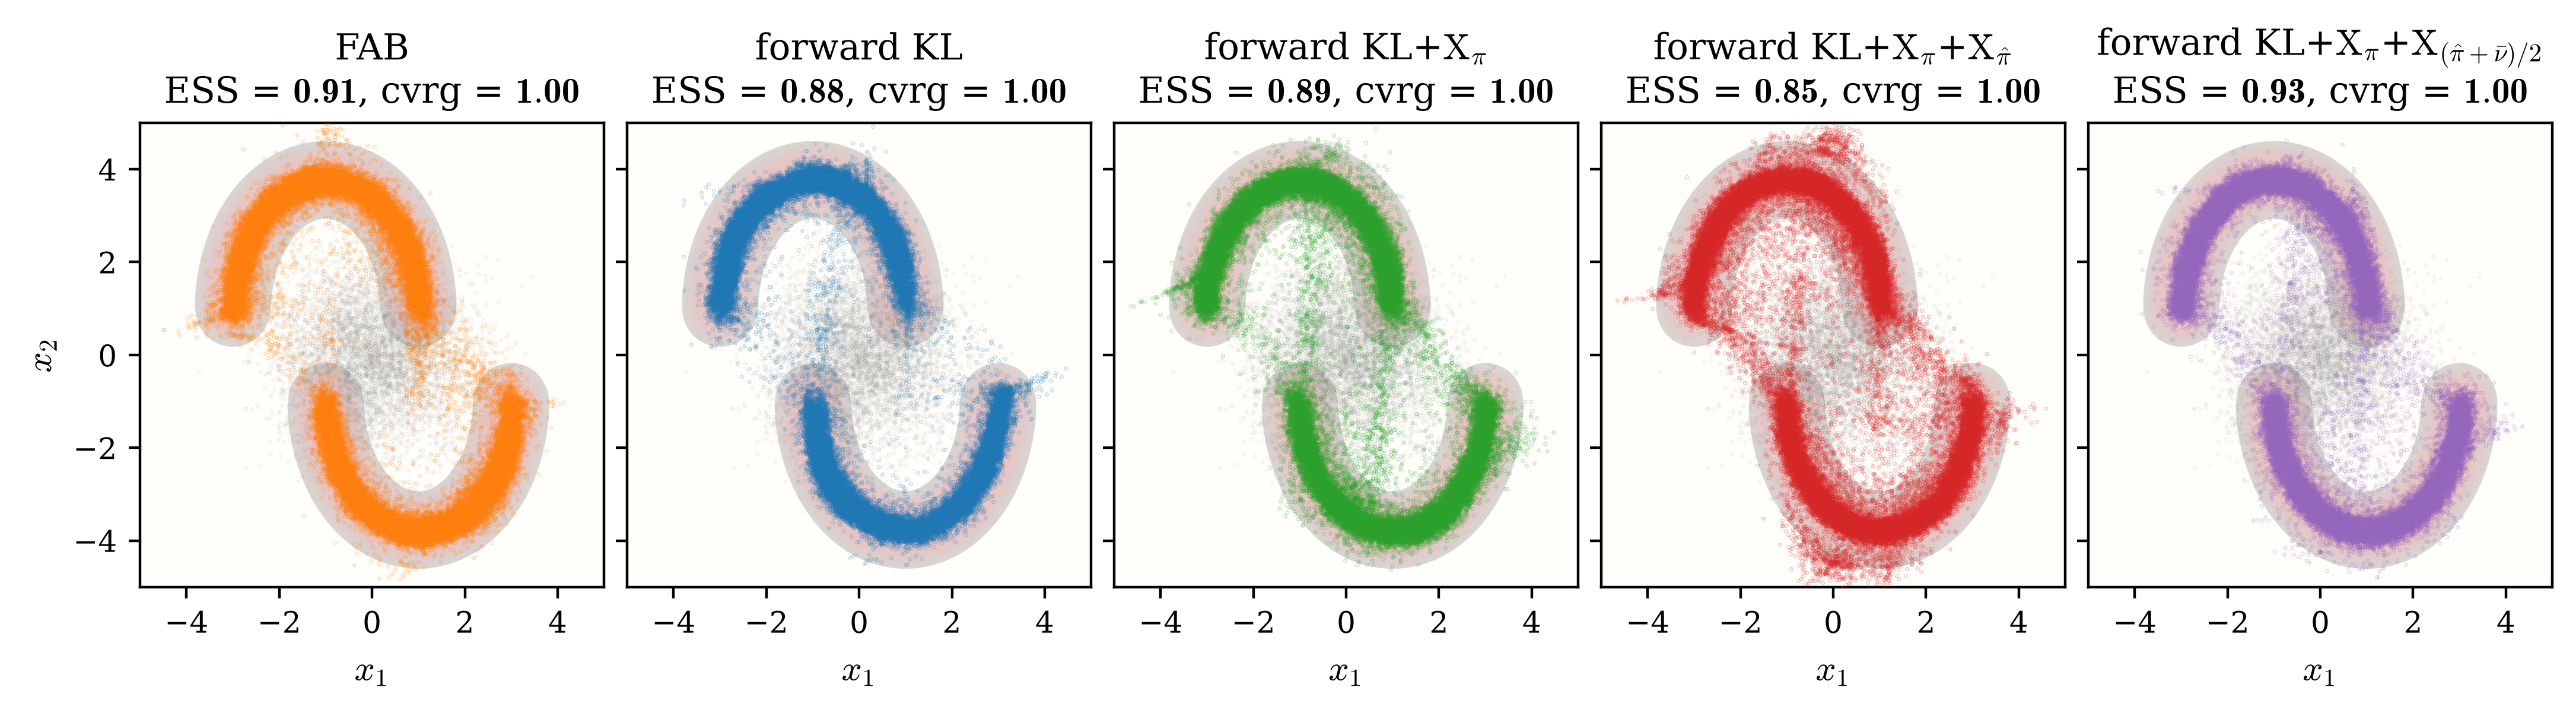
\includegraphics[width=\textwidth]{figures/2d_two_moon_samples.png}
    \caption{Two-Moon target. Columns, from left to right, are {\color{blue}FAB,} forward KL, $\KL$+$\X_\pi$, $\KL$+$\X_\pi$+$\X_{\hat\pi}$, and $\KL$+$\X_\pi$+$\X_{(\hat\pi+\bar\nu)/2}$. Each panel overlays the pushforward samples on the target energy and reports final ESS and coverage. Gray points show the source.}
    \label{fig: two-moon}
\end{figure}

\paragraph{Two-Moon.}
The source is $\mathcal N(0,I_2)$ and both crescents lie within its reach, so all four losses attain coverage $1$ (Figure~\ref{fig: two-moon}). With batch size $500$, $200$ Adam steps, and learning rate $10^{-3}$, forward KL reaches ESS $0.8934$, adding $\X_\pi$ leaves it at $0.8929$, and KLXX reaches $0.9087$. The loss $\KL$+$\X_\pi$+$\X_{\hat\pi}$ falls to $0.8313$, since QT supplies no mode that the target surrogate is missing.

\begin{figure}[htb]
    \centering
    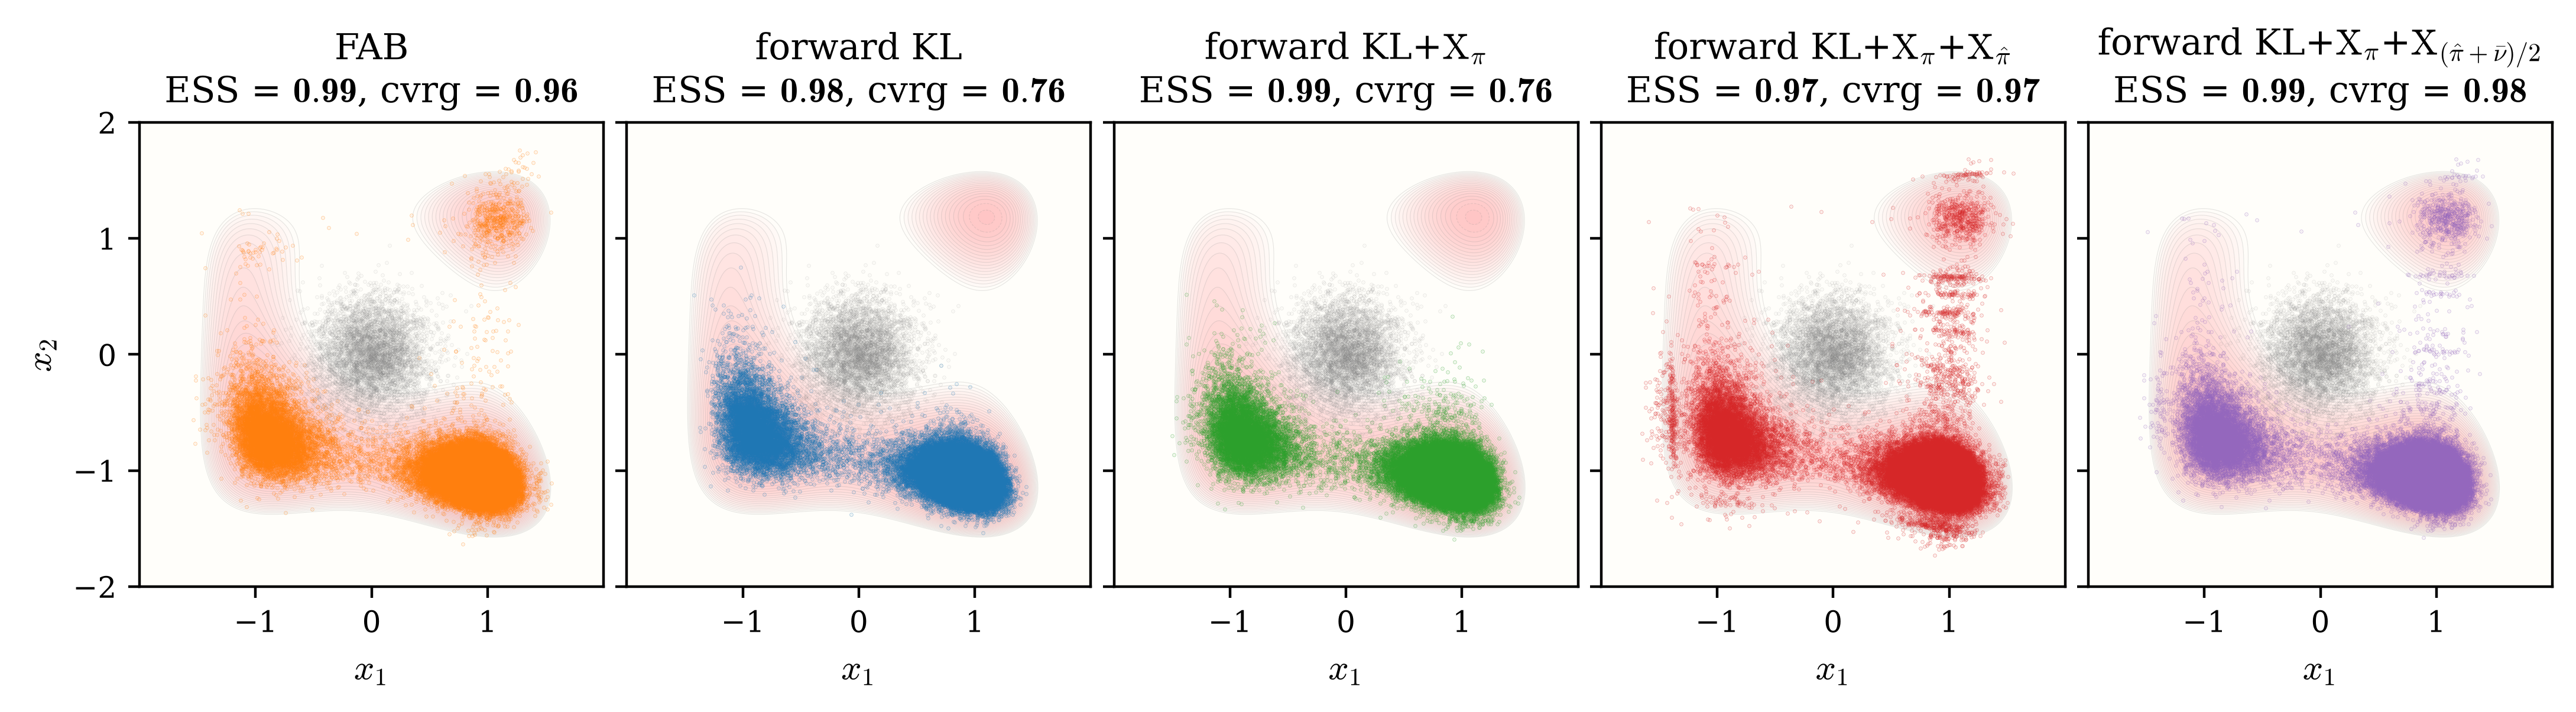
\includegraphics[width=\textwidth]{figures/2d_three_well_samples.png}
    \caption{Three-Well target. From left to right, the panels show {\color{blue}FAB,} forward KL, $\KL$+$\X_\pi$, $\KL$+$\X_\pi$+$\X_{\hat\pi}$, and $\KL$+$\X_\pi$+$\X_{(\hat\pi+\bar\nu)/2}$. Each panel overlays the pushforward samples on the target energy and reports final ESS and coverage; gray points show the source.}
    \label{fig: threewell}
\end{figure}

\paragraph{Three-Well.}
The source is $\mathcal N(0,0.25^2 I_2)$, narrower than the well separation and initially covering no basin (Figure~\ref{fig: threewell}). Training uses batch size $1000$, $500$ steps, and learning rate $10^{-3}$. Forward KL and $\KL$+$\X_\pi$ populate the two favored wells and report ESS $0.9769$ and $0.9939$, respectively, while their coverage remains $0.7595$. The QT set also represents the suppressed third well, and both losses that use it cover all three wells at comparable ESS.

\begin{figure}[htb]
    \centering
    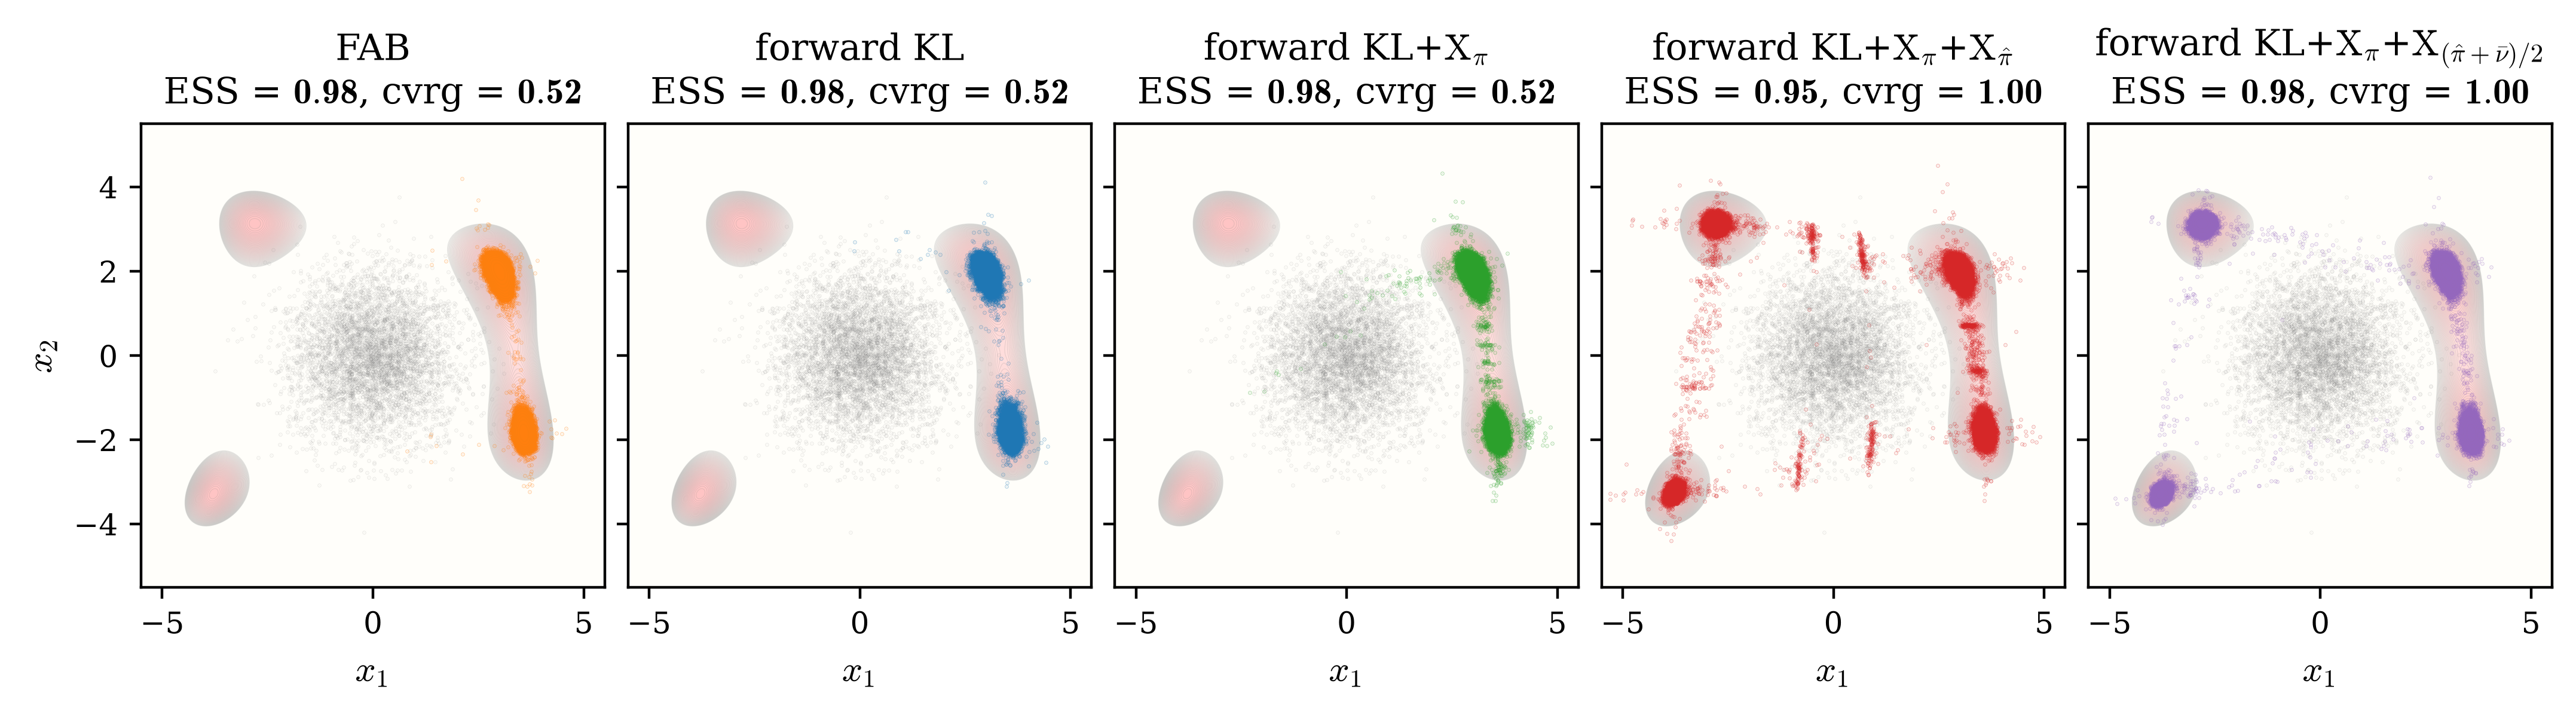
\includegraphics[width=\textwidth]{figures/2d_himmelblau_samples.png}
    \caption{Himmelblau target. Columns show {\color{blue}FAB,} forward KL, $\KL$+$\X_\pi$, $\KL$+$\X_\pi$+$\X_{\hat\pi}$, and $\KL$+$\X_\pi$+$\X_{(\hat\pi+\bar\nu)/2}$; each panel shows the pushforward samples over the target energy with final ESS and coverage, and gray points show the source.}
    \label{fig: himmelblau}
\end{figure}

\paragraph{Himmelblau.}
The source is $\mathcal N(0,I_2)$, whereas the four wells lie at radius approximately $3.6$--$5.0$. Training uses batch size $1000$, $1000$ steps, and learning rate $10^{-3}$. Forward KL and $\KL$+$\X_\pi$ capture only two wells, giving coverage $0.5160$ despite ESS $0.9814$ and $0.9596$. Both losses using $\hat\pi$ attain coverage $1$, and relative to $\KL$+$\X_\pi$+$\X_{\hat\pi}$, KLXX shows less intermodal mass and raises ESS from $0.9618$ to $0.9726$.
\begin{figure}[htb]
    \centering
    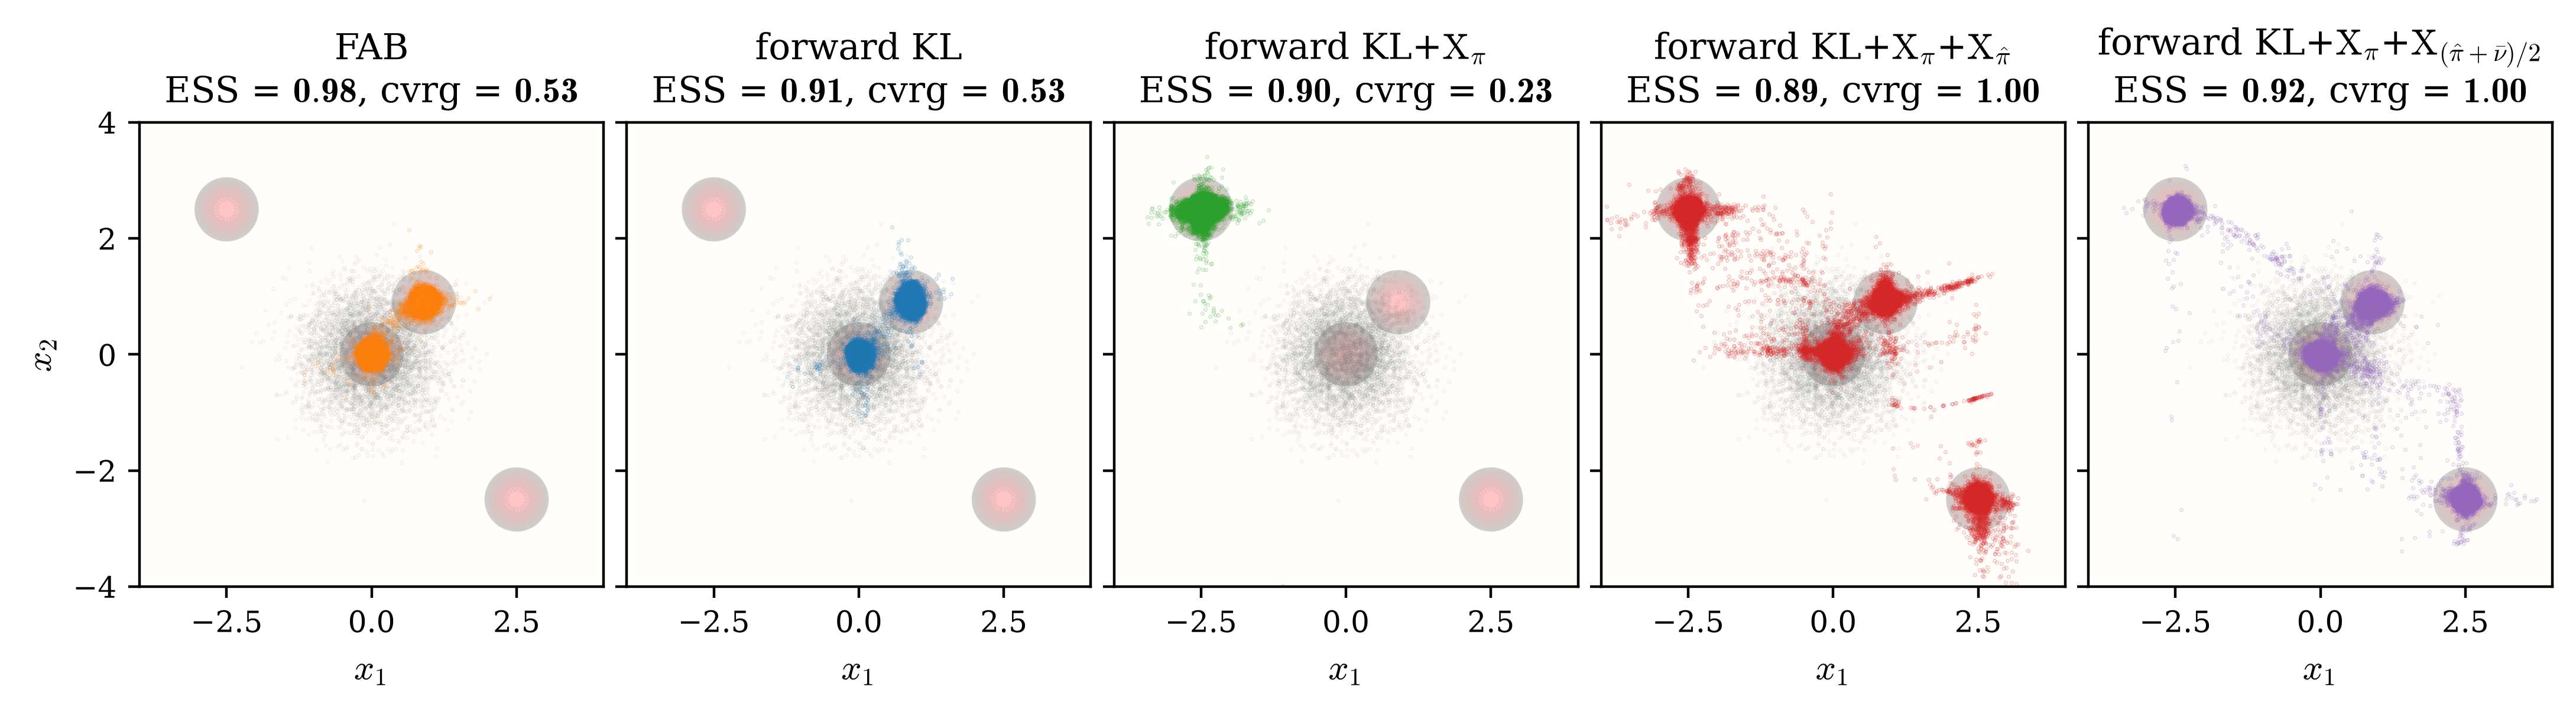
\includegraphics[width=\textwidth]{figures/2d_sparse_samples.png}
    \caption{Sparse target. Columns show {\color{blue}FAB,} forward KL, $\KL$+$\X_\pi$, $\KL$+$\X_\pi$+$\X_{\hat\pi}$, and $\KL$+$\X_\pi$+$\X_{(\hat\pi+\bar\nu)/2}$, with the pushforward samples overlaid on the target energy; panel titles report final ESS and coverage, and gray points show the source.}
    \label{fig: sparse}
\end{figure}


\paragraph{Sparse.}
The target is a four-component Gaussian mixture with component standard deviation $0.08$: two modes lie near the source center and two lie in opposite corners, more than five source standard deviations away. With source standard deviation $0.6$, batch size $1000$, $1000$ steps, and learning rate $5\times10^{-3}$, forward KL and $\KL$+$\X_\pi$ cover only the central pair, at coverage $0.5335$ and ESS $0.9031$ and $0.9567$. The loss $\KL$+$\X_\pi$+$\X_{\hat\pi}$ restores all four modes but places visible mass between them, at ESS $0.8783$, while KLXX attains coverage $1$ with less intermodal mass and ESS $0.9559$.

{\color{blue}We also run FAB \citep{midgley2022flow} on all four targets, with the same flow, source, target, batch size, step count, learning rate and MALA parameters as the losses above, so the runs differ only in the objective. Its annealing follows the geometric path from the pushforward distribution to $\pi^2/\nu$ through $\pi$, and it carries the prioritized replay buffer of the reference implementation. FAB discovers modes that forward KL does not, reaching the third Three-Well basin and one further mode on Himmelblau and on Sparse, which is what the mass-covering $2$-divergence is for. It does not reach every mode: one Himmelblau well stays empty at coverage $0.736$, and one far Sparse mode at $0.768$. Minimizing the $2$-divergence is minimizing importance weight variance, so at convergence FAB should hold the highest ESS here, and on Three-Well it does, at $0.985$; but it converges more slowly and each step costs more, and the shortest run, Two-Moon at $200$ steps, ends at $0.637$ against $0.83$ or above for every other method. The four targets support the intended division of labor in the KLXX loss: KLXX reaches every mode on every target, at the highest ESS among the mode-complete methods on three of the four.}

\begin{table}[htb]
    \centering
    \begin{tabular}{lccccc}
        \toprule
        target & {\color{blue}FAB} & KL & $\KL$+$\X_\pi$ & $\KL$+$\X_\pi$+$\X_{\hat\pi}$ & $\KL$+$\X_\pi$+$\X_{(\hat\pi+\bar\nu)/2}$ \\
        \midrule
        Two-Moon   & {\color{blue}$0.637\,(1.000)$} & $0.893\,(1.000)$ & $0.893\,(1.000)$ & $0.831\,(1.000)$ & $\mathbf{0.909}\,(1.000)$ \\
        Three-Well & {\color{blue}$\mathbf{0.985}\,(0.961)$} & $0.977\,(0.760)$ & $0.994\,(0.760)$ & $0.968\,(0.977)$ & $0.982\,(0.971)$ \\
        Himmelblau & {\color{blue}$0.889\,(0.736)$} & $0.981\,(0.516)$ & $0.960\,(0.516)$ & $0.962\,(1.000)$ & $\mathbf{0.973}\,(1.000)$ \\
        Sparse     & {\color{blue}$0.690\,(0.768)$} & $0.903\,(0.534)$ & $0.957\,(0.534)$ & $0.878\,(1.000)$ & $\mathbf{0.956}\,(1.000)$ \\
        \bottomrule
    \end{tabular}
    \caption{Final ESS, with $\kappa=5$ coverage in parentheses, on the four 2D targets. Bold marks the highest ESS among methods whose sample panel covers every target mode. {\color{blue}Mode completeness is read from the panels rather than from the coverage number, which undercounts the visibly occupied third mode on Three-Well.}}
    \label{tab: 2d-benchmark-summary}
\end{table}

The mechanism behind that division of labor is visible term by term. Adding $\X_\pi$ leaves ESS near the forward KL value on Two-Moon, where coverage is already complete. QT samples supply information about modes absent from the target surrogate. Adding the pushforward samples to that mixture reduces visible intermodal mass relative to $\KL$+$\X_\pi$+$\X_{\hat\pi}$.

\subsection{High-dimensional product multi-well}
\label{subsec: highd}

We next isolate accuracy scaling over the dimensions
$d=16,32,48,\ldots,256$. Letting $k=\lfloor\log_2 d\rfloor$, we use
\begin{equation}
    U(\mathbf{x})=\frac12\lVert\mathbf{x}\rVert^2
    +12\sum_{i=1}^{k}\exp(-x_i^2).
    \label{eq: highd-potential}
\end{equation}
The first $k$ coordinates are symmetric double wells with minima at $\pm\sqrt{\ln 24}$ and barrier approximately $9.9$, while the remaining $d-k$ coordinates are standard Gaussian. The target therefore has exactly $2^k$ equal-weight sign-pattern modes, where $2^k\Le d<2^{k+1}$. Multimodality occupies only a $k$-dimensional subspace, but the log-weight error accumulates across all $d$ coordinates.

All four losses use the same identity-initialized NSF on $[-4,4]^d$, with $16$ bins, $6$ transforms, and conditioner widths $(256,256)$. At every dimension, training uses batch size $250$, $2000$ Adam steps at learning rate $10^{-3}$, and a fixed sample set of size $5000d$. The target surrogate uses a ladder of length $M=1$ followed by $50$ MALA steps of size $2\times10^{-3}$. QT uses $1000d$ samples, melt scale $2$, and an L-BFGS quench with initial step $0.5$ and $200$ iterations. Final sample ESS is evaluated on $80000$ fresh source samples. Each loss--dimension pair is one fixed-seed training realization.

\begin{figure}[htb]
    \centering
    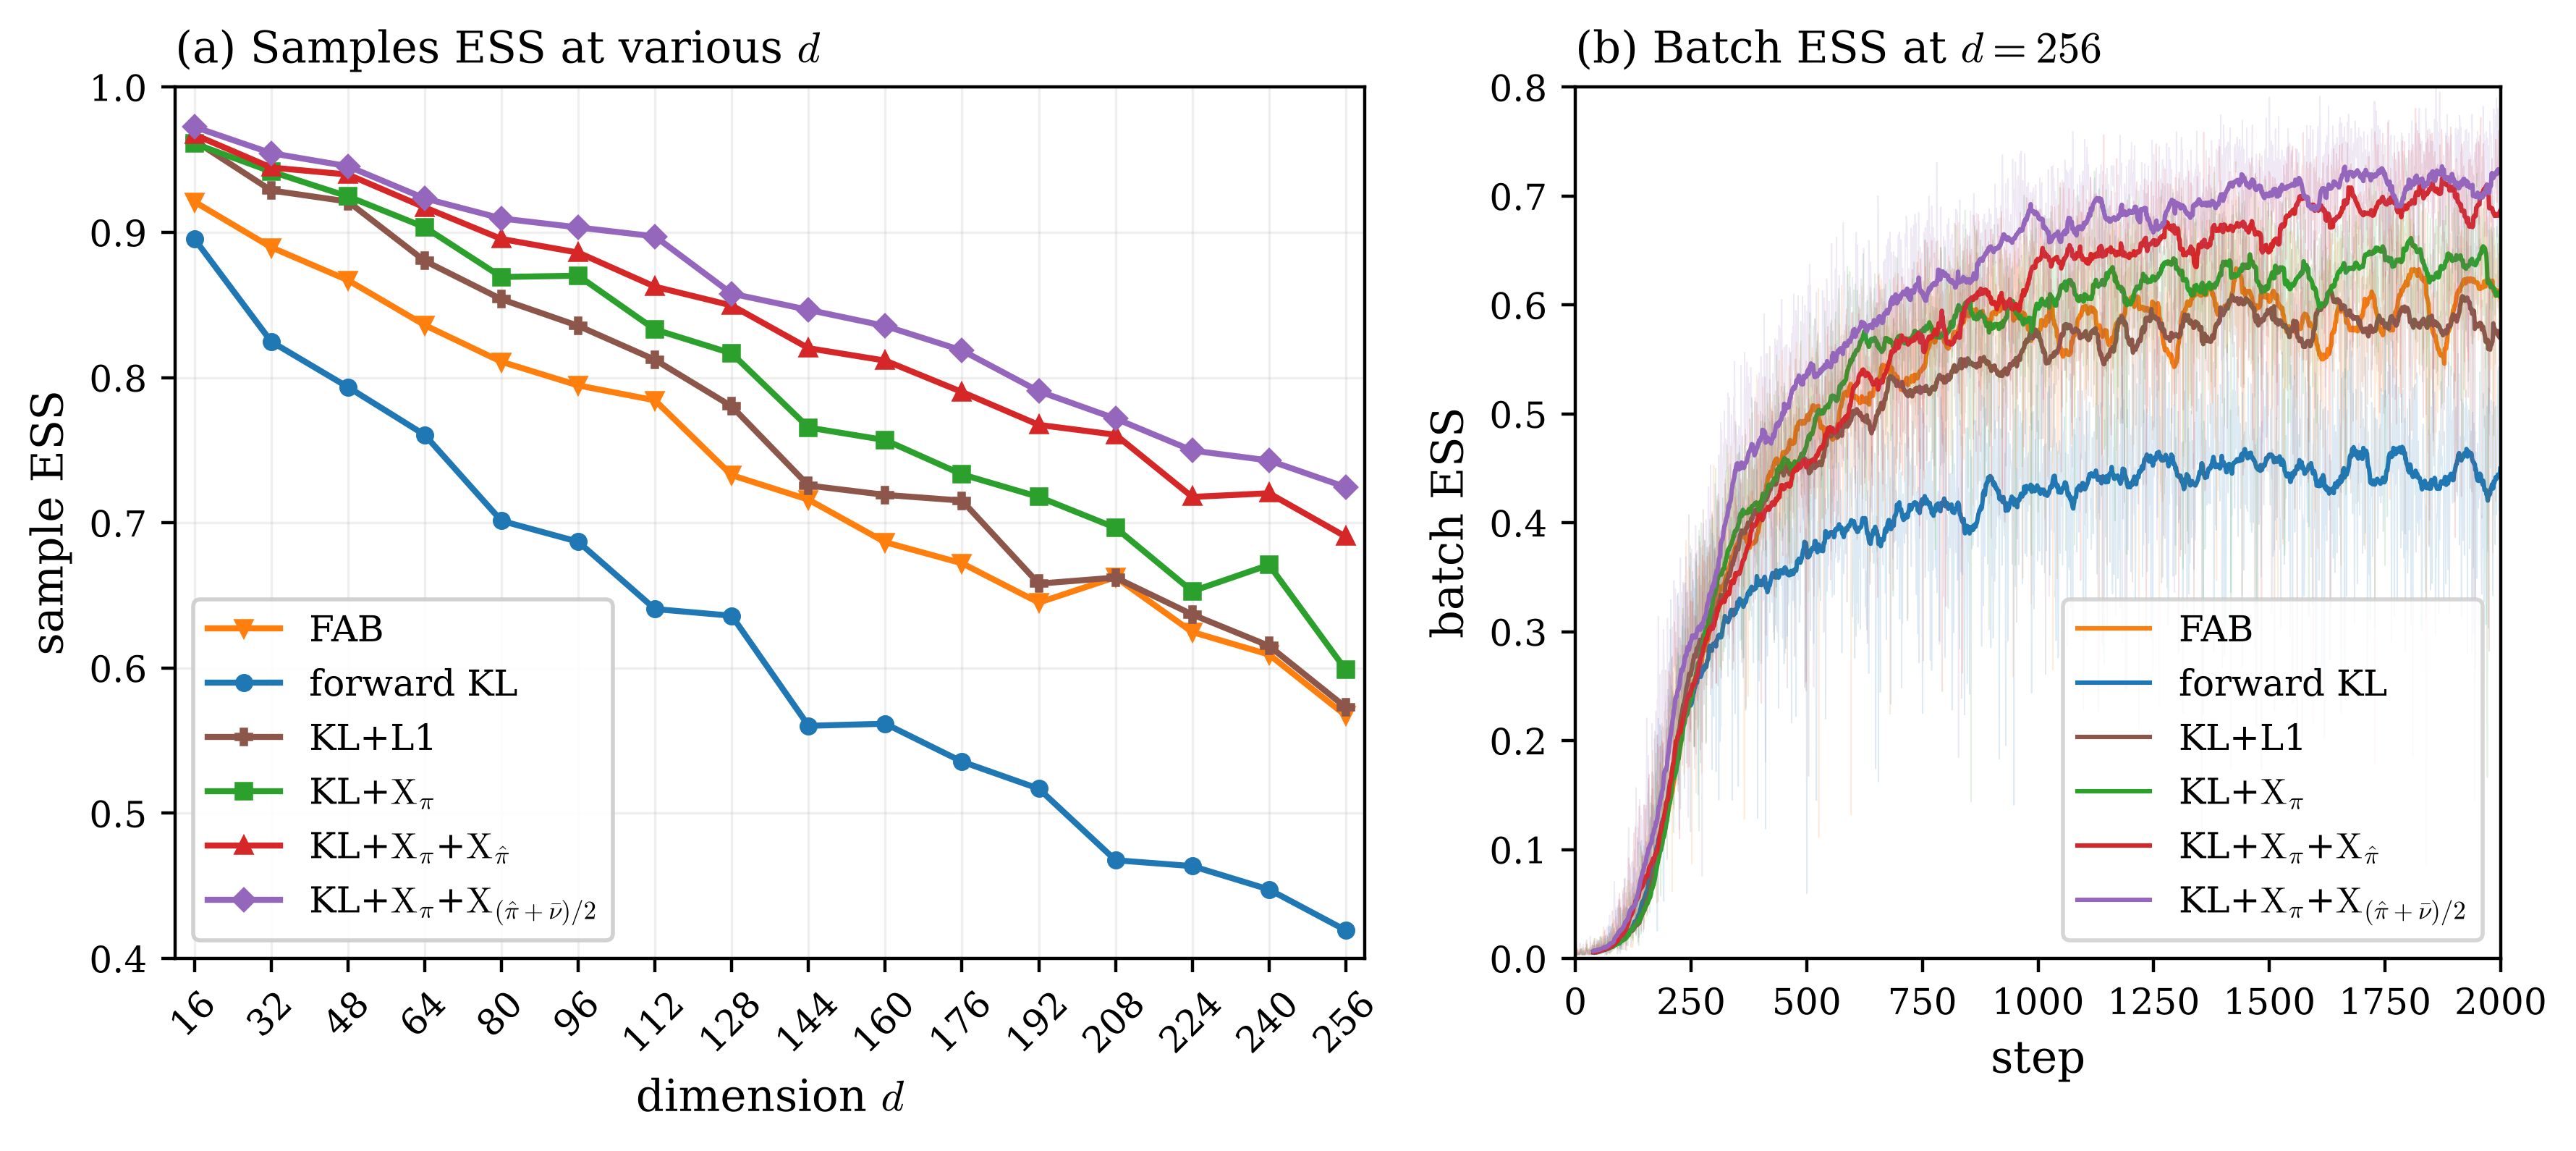
\includegraphics[width=\textwidth]{figures/hd_product_ess.png}
    \caption{ESS on the product multi-well target \eqref{eq: highd-potential}. (a) Final sample ESS over sixteen tested dimensions. (b) Batch ESS during the $d=256$ training; bold curves are $40$-step moving averages of the raw values.}
    \label{fig: highd-ess}
\end{figure}

{\color{blue}The coverage diagnostic of Section~\ref{subsec: eval} is not used here. Nearest-neighbor radii concentrate as the dimension grows, so a $\kappa$-nearest-neighbor ball ceases to separate covered from uncovered regions, and the sign pattern of the double-well coordinates is the exact mode label for this target and is read directly.} In each of the $64$ evaluated pairs of loss and dimension, all $2^k$ sign patterns of the double-well coordinates occur among the fresh evaluation samples, including all $256$ patterns for each of the four losses at $d=256$. Figure~\ref{fig: highd-ess} shows that each of the three losses with log-ratio variation has higher final sample ESS than forward KL at every one of the sixteen dimensions. At $d=256$, the final values are $0.4322$ for forward KL, $0.5608$ for $\KL$+$\X_\pi$, $0.5979$ for $\KL$+$\X_\pi$+$\X_{\hat\pi}$, and $0.5687$ for $\KL$+$\X_\pi$+$\X_{(\hat\pi+\bar\nu)/2}$. The two losses containing $\hat\pi$ behave similarly across dimensions. During the $d=256$ training realization, the batch ESS of $\KL$+$\X_\pi$, evaluated on the training batch after each gradient step, rises more slowly than that of forward KL over the first several hundred steps and overtakes it only near step $800$. Adding $\X_{\hat\pi}$ removes that delay: both losses containing $\hat\pi$ overtake forward KL earlier, and the mixture term does so first. All three losses with log-ratio variation then continue to improve after forward KL begins to plateau.

\subsection{Lattice \texorpdfstring{$\phi^4$}{phi4} field theory: fake ESS at a collective barrier}
\label{subsec: phi4}
On a periodic $L\times L$ lattice with $d=L^2$, the tilted scalar $\phi^4$ action is
\begin{equation*}
U(\boldsymbol\phi)
=-0.8\sum_{\langle jl\rangle}\phi_j\phi_l
+\sum_{j=1}^{d}\left[\phi_j^2+\frac12(\phi_j^2-1)^2\right]
+h\sum_{j=1}^{d}\phi_j.
\end{equation*}
The on-site term alone has a single minimum at $0$; the nearest-neighbor coupling is what makes a uniform configuration bistable. The magnetization of a configuration is
\begin{equation*}
    m(\boldsymbol\phi)=\frac1d\sum_{j=1}^{d}\phi_j .
\end{equation*}
We take $h=0.0257$ at $L=6$ and $h=0.0144$ at $L=8$, matching the scaling $hL^2\approx0.92$ to produce comparable well imbalance in the targets of the two settings.
A collective domain-wall barrier separates the two wells, and the minority weight $p_+=\mathbb P(m>0)$ must be learned rather than fixed by symmetry.

PT provides the references $p_+=0.1258\pm0.0001$ for $L=6$ and $0.1265\pm0.0002$ for $L=8$, with 3 independent runs for both $L$. Each loss uses an identity-initialized NSF on $[-3,3]^d$, with $16$ bins, $6$ transforms, and conditioner widths $(256,256)$. The source is $\mathcal N(0,0.5^2 I_d)$; training uses a fixed sample set of $10^5$ source samples, batch size $500$, and $2000$ Adam steps at learning rate $10^{-3}$. The target surrogate uses a ladder of length $M=1$ followed by $50$ MALA steps of size $2\times10^{-3}$. QT acts on the sample set, with melt scale $2$ and an L-BFGS quench using initial step $0.1$ and $200$ iterations.

\begin{table}[htb]
    \centering
    \begin{tabular}{lcccc}
        \toprule
        & \multicolumn{2}{c}{$L=6$} & \multicolumn{2}{c}{$L=8$} \\
        \cmidrule(lr){2-3}\cmidrule(lr){4-5}
        & ESS & $p_+$ & ESS & $p_+$ \\
        \midrule
        forward KL
        & $0.794/0.840/0.826$ & $1/1/0$
        & $0.622/0.686/0.684$ & $1/0/1$ \\
        $\KL$+$\X_\pi$
        & $0.935/0.933/0.945$ & $1/1/0$
        & $0.804/0.824/0.821$ & $1/0/0$ \\
        $\KL$+$\X_\pi$+$\X_{\hat\pi}$
        & $0.875/0.873/0.871$ & $0.127/0.128/0.127$
        & $0.636/0.645/0.654$ & $0.125/0.124/0.124$ \\
        $\KL$+$\X_\pi$+$\X_{(\hat\pi+\bar\nu)/2}$
        & $0.896/0.877/0.894$ & $0.127/0.128/0.127$
        & $0.690/0.676/0.681$ & $0.131/0.130/0.129$ \\
        \midrule
        PT reference & --- & $0.1258\pm0.0001$ & --- & $0.1265\pm0.0002$ \\
        \bottomrule
    \end{tabular}
    \caption{Final ESS and reweighted minority-well weight $p_+$ for three seeds on the two tilted $\phi^4$ targets, $(L,h)=(6,0.0257)$ and $(8,0.0144)$. Integer values $0$ and $1$ indicate collapse onto one well.}
    \label{tab: phi4}
\end{table}

Forward KL and $\KL$+$\X_\pi$ collapse at every size and seed (Table~\ref{tab: phi4}). Their target surrogate starts from the pushforward samples and does not cross the collective barrier within the run, so the second well remains absent and reweighting gives $p_+=0$ or $1$. Nevertheless, $\KL$+$\X_\pi$ has the highest ESS at both sizes, and it is a fake ESS: it is earned on the single well the flow reaches, and the missing one does not enter it. KLXX populates both wells, so its ESS  accurately reflects the quality of the samples.

\begin{figure}[htb]
    \centering
    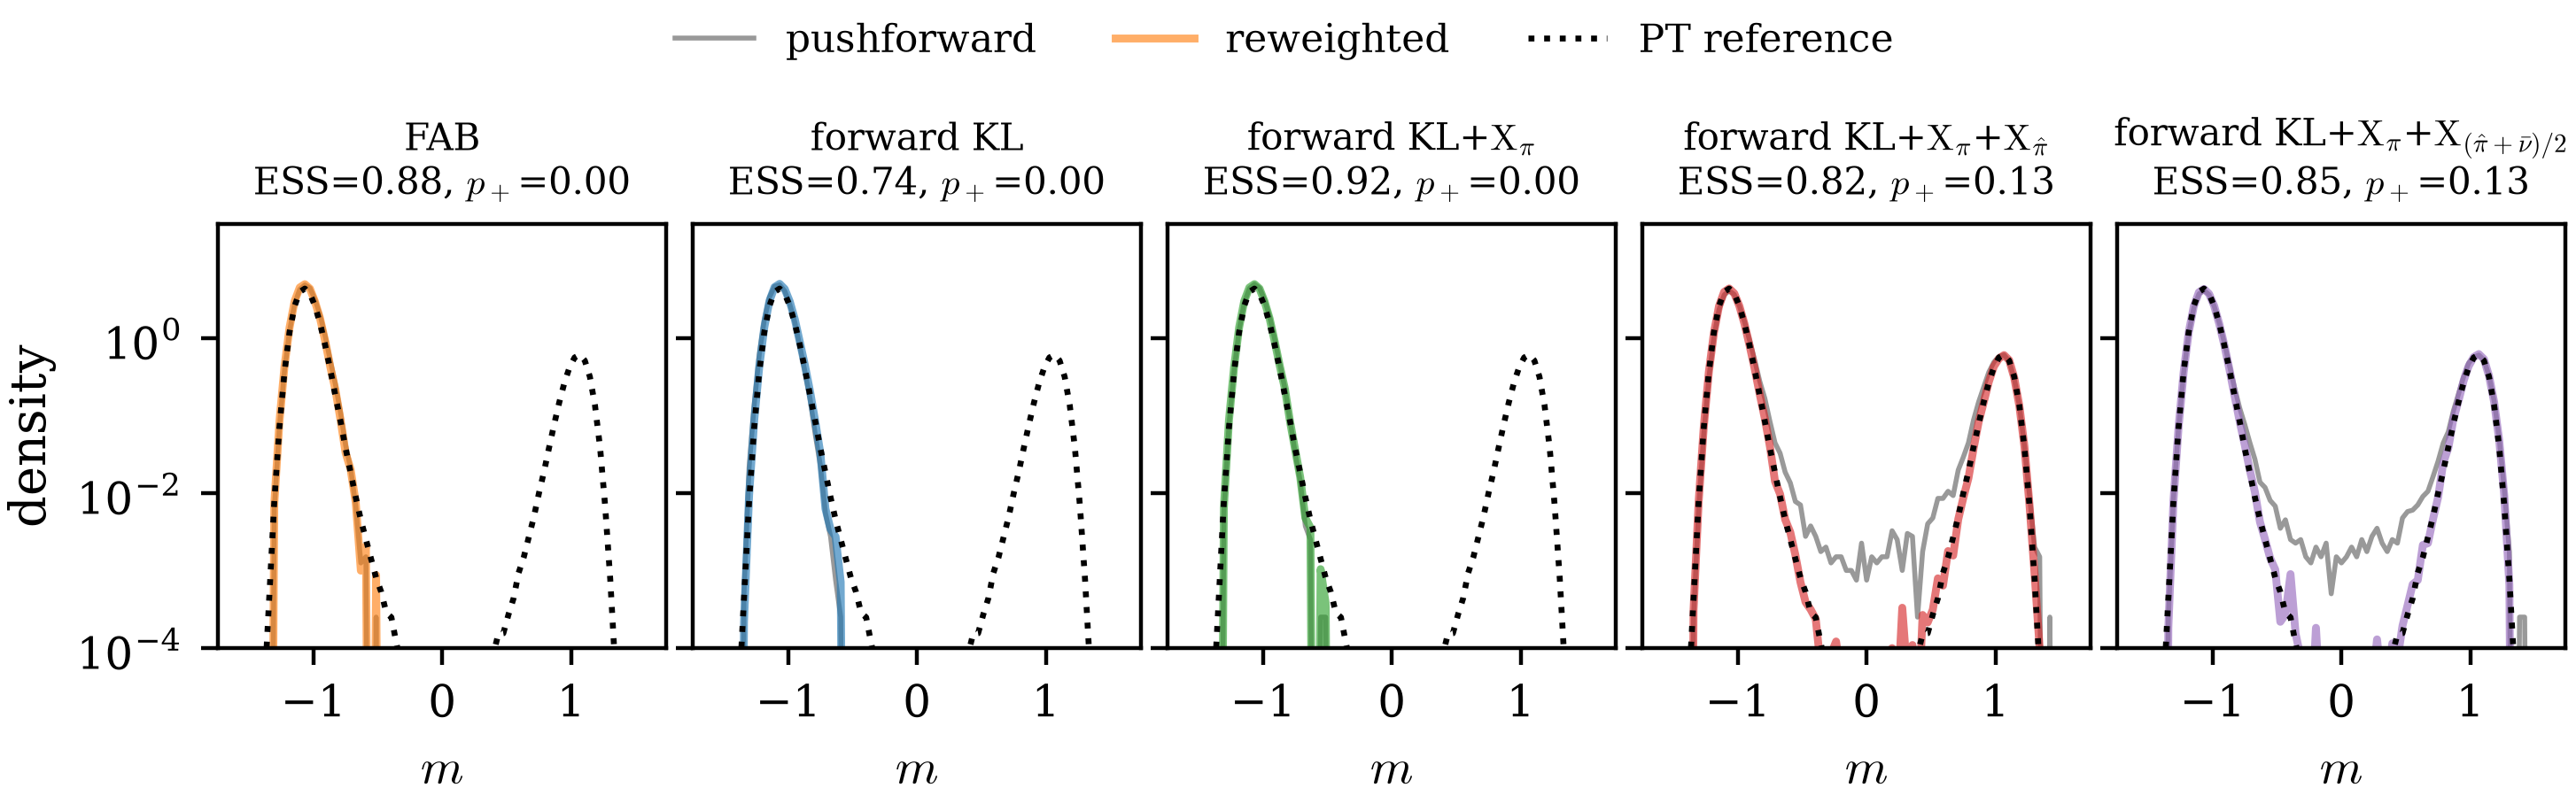
\includegraphics[width=\textwidth]{figures/lattice_phi4_l8_methods.png}
    \caption{Magnetization density on the $L=8$ lattice. Each panel shows the pushforward density (gray), the reweighted density (color), and the PT reference density (dotted); the title reports ESS and reweighted $p_+$.}
    \label{fig: phi4-methods}
\end{figure}

The two losses that use the QT samples $\hat\pi$ populate both wells at every seed, with recovered $p_+$ between $0.1238$ and $0.1312$, within $0.005$ of the reference at the corresponding lattice size. In these finite-capacity fits, recovering both wells is accompanied by some mass in the suppressed region between them and lower ESS. At $L=8$, KLXX has the higher ESS and less visible mass in that region (Figure~\ref{fig: phi4-methods}), matching the role of the pushforward samples in the mixture variation.

\subsection{Boltzmann generator on \texorpdfstring{$p$}{p}-state clock model}
\label{subsec: clock}

The preceding benchmarks use a single flow. We now test the full adaptive-staging construction on the $p=6$ clock model on a periodic $8\times8$ lattice,
\begin{equation}
U(\boldsymbol\theta)
=-\sum_{\langle jl\rangle}\cos(\theta_j-\theta_l)
-\frac12\sum_{j=1}^{d}\cos(6\theta_j),
\qquad \boldsymbol\theta\in[-\pi,\pi)^{d},\qquad d=64,
\label{eq: clock-potential}
\end{equation}
where $\langle jl\rangle$ runs over nearest-neighbor pairs. The source is uniform on the torus and the interpolation is $U_t=tU$. The target distribution $\pi\propto\exp(-U)$ separates into six symmetry-related clock sectors.

Each stage uses an identity-initialized neural circular spline flow with $16$ bins, $6$ autoregressive transforms, and conditioner widths $(256,256)$. The sample set contains $4\times10^5$ samples, and both SMC and QT act directly on this set. Every stage uses $3000$ Adam steps at learning rate $10^{-3}$ and ladder length $M=4$ for both the adaptive SMC screen and the target surrogate, with $100$ MALA steps of size $10^{-3}$. For KLXX, QT uses melt scale $2\pi$ and an L-BFGS quench with initial step $10^{-2}$ and $100$ iterations. The clock stage schedule uses the nondefault settings $t_{\mathrm{safe}}=0.25$, enlarge factor $\Gamma=2$, and SMC gate $\tau_{\mathrm{SMC}}=0.7$, {\color{blue}with the ESS gate at its default $\tau_{\mathrm v}=0.4$}. We report batch sizes $B=2000,1000,500,250$.

KLXX uses the same stage schedule as forward KL for fair comparison. That schedule is constructed with forward KL under the adaptive SMC screen with the ESS gate $\tau_{\mathrm v}=0.4$, and KLXX is trained on the identical accepted values of $t$. Every configuration is a single run, so individual stage ESS values carry single-run fluctuation.

The principal diagnostic is the sample ESS of each accepted stage. The propagation factor $\hat F_\Sigma$ of \eqref{eq: propagation-factor-hat} summarizes stagewise weight degeneracy across the stage sequence; smaller is better. It is not a full-chain ESS or an endpoint error estimate. Table~\ref{tab: clock-summary} reports every accepted stage and the resulting factor.

\begin{table}[htb]
    \centering
    \begin{tabular}{lccccccccc}
        \toprule
        stage $k$ & 1 & 2 & 3 & 4 & 5 & 6 & 7 & 8 & $\hat F_\Sigma$ \\
        \midrule
        $t_k$ ($B=2000$) & 0.250 & 0.495 & 0.663 & 0.779 & 0.887 & 1.000 & --- & --- & \\
        forward KL & 0.751 & 0.570 & 0.471 & 0.474 & 0.511 & 0.602 & --- & --- & 21.4 \\
        $\KL$+$\X_\pi$+$\X_{(\hat\pi+\bar\nu)/2}$ & $\mathbf{0.921}$ & $\mathbf{0.759}$ & $\mathbf{0.608}$ & $\mathbf{0.562}$ & $\mathbf{0.558}$ & $\mathbf{0.649}$ & --- & --- & $\mathbf{15.6}$ \\
        \midrule
        $t_k$ ($B=1000$) & 0.250 & 0.495 & 0.613 & 0.728 & 0.841 & 0.952 & 1.000 & --- & \\
        forward KL & 0.672 & 0.479 & 0.580 & 0.463 & 0.427 & 0.520 & 0.830 & --- & 28.3 \\
        $\KL$+$\X_\pi$+$\X_{(\hat\pi+\bar\nu)/2}$ & $\mathbf{0.866}$ & $\mathbf{0.642}$ & $\mathbf{0.700}$ & $\mathbf{0.545}$ & $\mathbf{0.462}$ & $\mathbf{0.541}$ & $\mathbf{0.859}$ & --- & $\mathbf{21.2}$ \\
        \midrule
        $t_k$ ($B=500$) & 0.250 & 0.421 & 0.590 & 0.705 & 0.784 & 0.895 & 1.000 & --- & \\
        forward KL & 0.580 & 0.549 & 0.408 & 0.432 & 0.525 & 0.417 & 0.530 & --- & 40.7 \\
        $\KL$+$\X_\pi$+$\X_{(\hat\pi+\bar\nu)/2}$ & $\mathbf{0.778}$ & $\mathbf{0.695}$ & $\mathbf{0.506}$ & $\mathbf{0.500}$ & $\mathbf{0.595}$ & $\mathbf{0.429}$ & $\mathbf{0.566}$ & --- & $\mathbf{29.3}$ \\
        \midrule
        $t_k$ ($B=250$) & 0.250 & 0.421 & 0.539 & 0.654 & 0.734 & 0.811 & 0.887 & 1.000 & \\
        forward KL & 0.468 & 0.448 & 0.495 & 0.428 & 0.506 & 0.484 & 0.514 & 0.424 & 62.7 \\
        $\KL$+$\X_\pi$+$\X_{(\hat\pi+\bar\nu)/2}$ & $\mathbf{0.659}$ & $\mathbf{0.586}$ & $\mathbf{0.601}$ & $\mathbf{0.480}$ & $\mathbf{0.563}$ & $\mathbf{0.536}$ & $\mathbf{0.564}$ & $\mathbf{0.464}$ & $\mathbf{41.7}$ \\
        \bottomrule
    \end{tabular}
    \caption{Stage ESS, the sample ESS of the map selected at a stage, on every accepted stage of the schedule-matched clock-model comparison between forward KL and $\KL$+$\X_\pi$+$\X_{(\hat\pi+\bar\nu)/2}$. Within each batch size block, both losses traverse the listed stage schedule. The final column is the propagation factor $\hat F_\Sigma$ in \eqref{eq: propagation-factor-hat}; bold marks the better loss at each stage and the smaller propagation factor.}
    \label{tab: clock-summary}
\end{table}

KLXX has higher sample ESS on all $28$ shared stages, raising the geometric mean stage ESS from $0.556$ to $0.665$ at $B=2000$, from $0.553$ to $0.643$ at $B=1000$, from $0.487$ to $0.571$ at $B=500$, and from $0.470$ to $0.553$ at $B=250$. It reduces the propagation factor $\hat F_\Sigma$ at every reported batch size, by ratios between $1.33$ and $1.50$: the factor falls from $21.4$ to $15.6$ at the largest batch and from $62.7$ to $41.7$ at the smallest. As the batch shrinks, the schedule lengthens and both propagation factors grow.

\begin{figure}[htb]
    \centering
    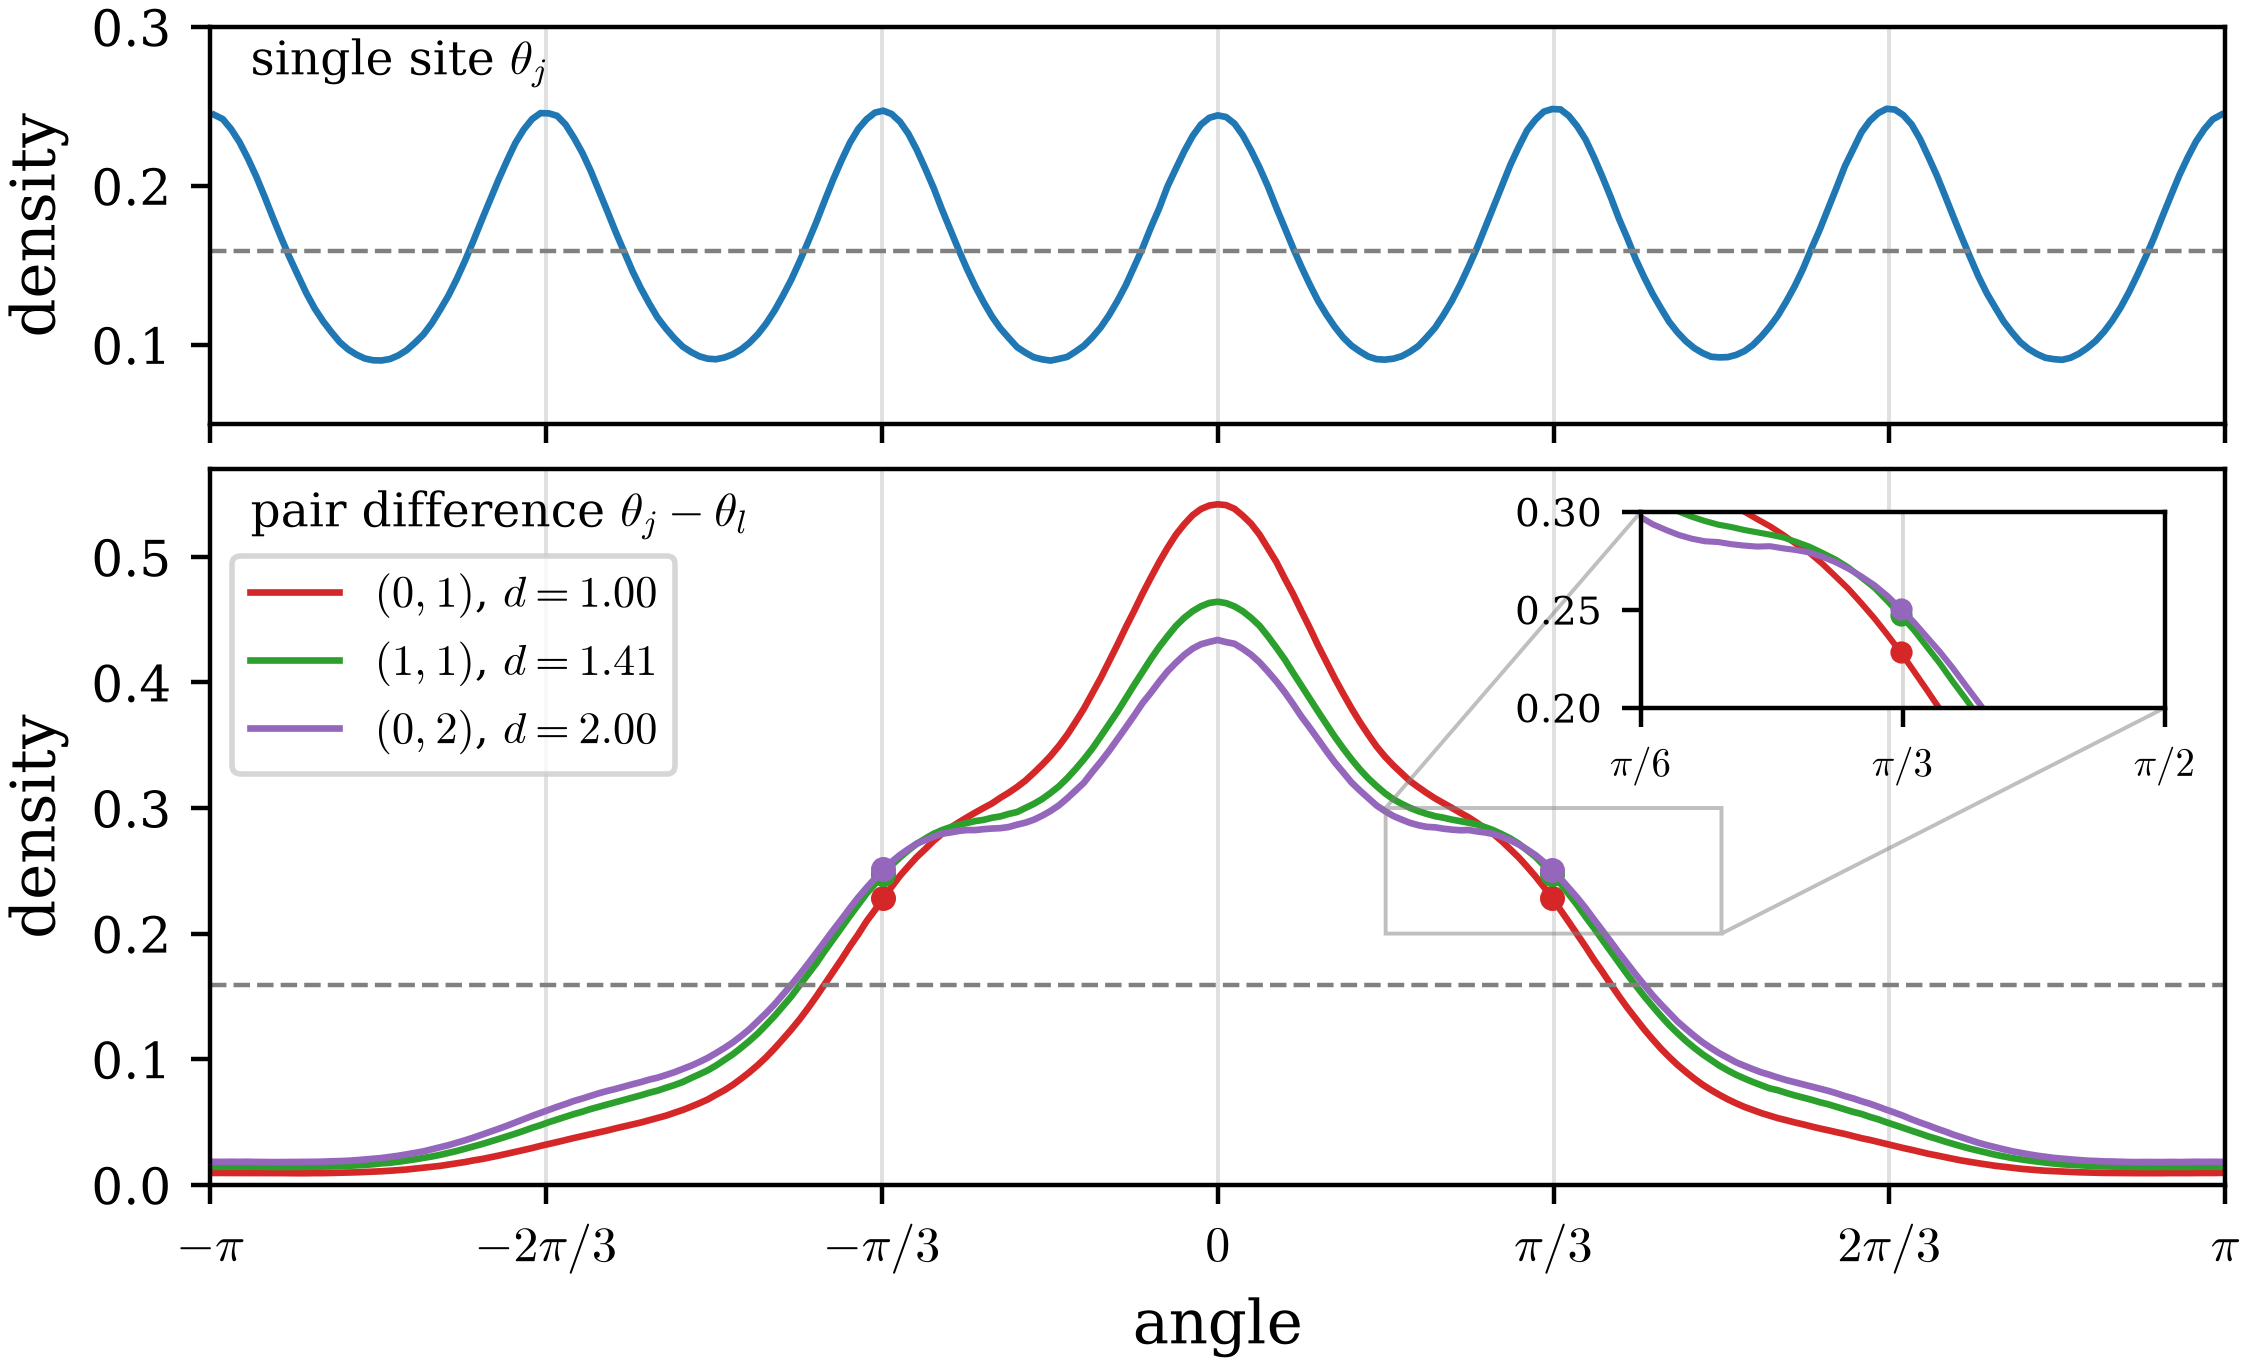
\includegraphics[width=0.7\textwidth]{figures/lattice_clock_marginals.png}
    \caption{Angle densities from $2\times10^6$ fresh samples advanced through the trained $B=2000$ $\KL$+$\X_\pi$+$\X_{(\hat\pi+\bar\nu)/2}$ stage sequence by map, reweighting, resampling, and MALA. The upper panel is the single-site marginal. The lower panel gives pair differences at offsets $(0,1)$, $(1,1)$, and $(0,2)$; dots and the inset resolve the one-clock-step angle $\pi/3$. Dashed lines show the uniform density.}
    \label{fig: clock-marginals}
\end{figure}


The single-site marginal exhibits all six clock wells with nearly equal peak heights. Pair differences are most concentrated at zero for nearest neighbors; as the lattice separation increases, the alignment peak falls and the shoulders near $\pm\pi/3$ gain mass. This is the expected decay of local angular order with distance.

To quantify whether staged resampling preserves the sixfold symmetry, we perform two fresh-rebuild tests through the trained stage sequences. The batch size test fixes $N=6.4\times10^5$, uses $B\in\{2000,1000,500,250\}$, and averages over four matched sampling seeds for each method and batch size. The particle-count test fixes $B=2000$ and uses $N=10^4\,2^k$, $k=0,\ldots,6$, with $2^{8-k}$ independent rebuilds at each size so every particle-count value has equal total work of $2.56\times10^6$ particles. For each sample, let $s$ be the clock sector nearest to the argument of the complex magnetization $d^{-1}\sum_{j=1}^d e^{\mathrm i\theta_j}$, and let $p_s$ be the empirical fraction assigned to sector $s$. We define
\[
\operatorname{occupancy\ bias}:=\frac16\sum_{s=0}^{5}\left|p_s-\frac16\right|.
\]

\begin{figure}[htb]
    \centering
    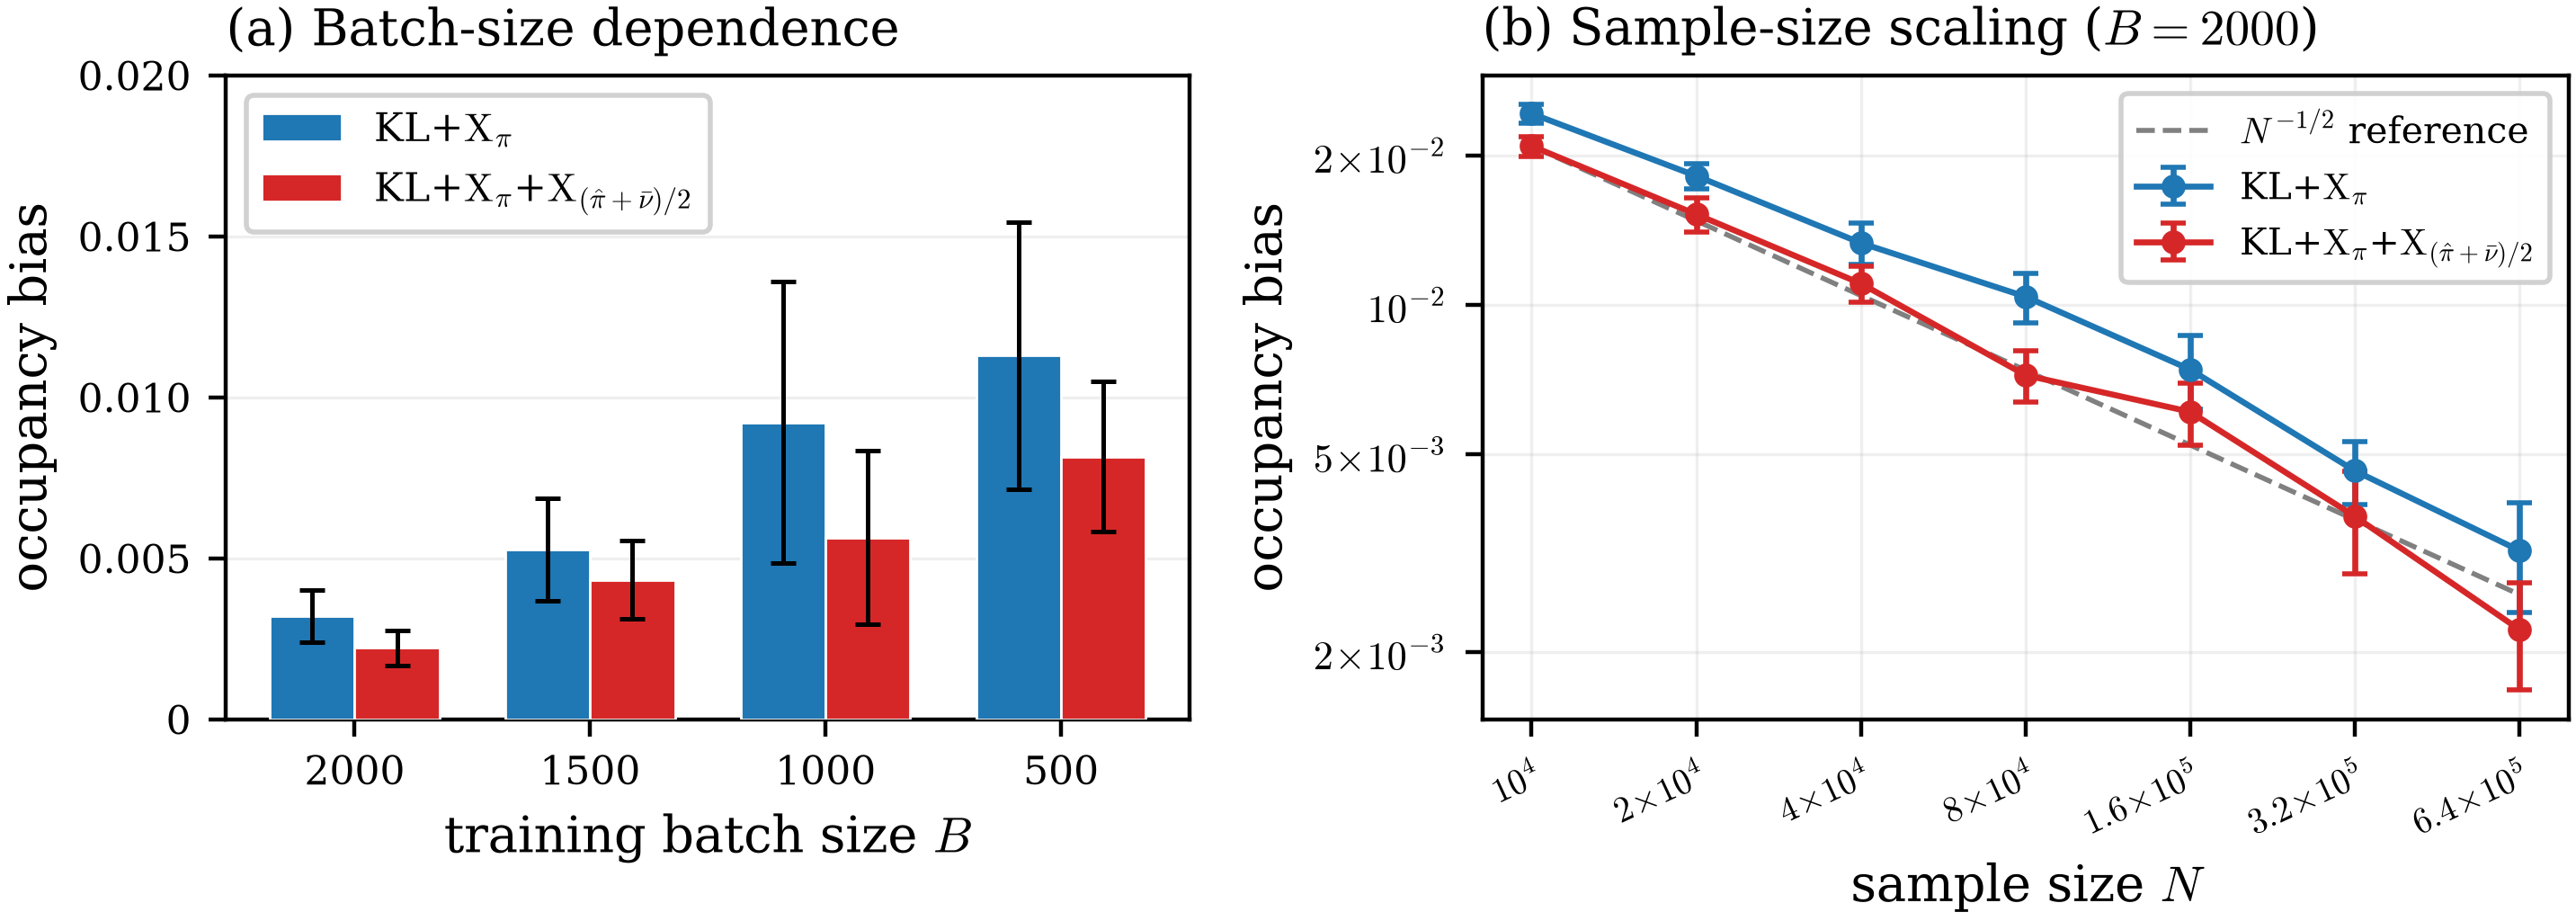
\includegraphics[width=0.9\textwidth]{figures/lattice_clock_occupancy_bias.png}
    \caption{Clock-sector occupancy bias under two fresh-rebuild tests. (a) Mean bias at fixed $N=6.4\times10^5$ across training batch sizes; each bar averages four matched sampling seeds. (b) Mean bias at fixed $B=2000$ versus particle count; at $N=2^k\times10^4$, each mean uses $2^{8-k}$ independent rebuilds, keeping the total work per point at $2.56\times10^6$ particles. Error bars in both panels are $\pm2$ standard errors. The dashed line in (b) is an $N^{-1/2}$ reference. The two panels' numbers align at $B=2000$, $N=6.4\times10^5$.}
    \label{fig: clock-occupancy}
\end{figure}


At fixed $N$, panel (a) of Figure~\ref{fig: clock-occupancy} shows that the mean occupancy bias increases as the training batch shrinks for both methods. KLXX has the lower mean at $B=2000$, $1000$, and $250$. At those batch sizes, the forward KL means are $0.00573$, $0.00888$, and $0.02760$, while the KLXX means are $0.00235$, $0.00517$, and $0.01506$. At $B=500$ the ordering reverses slightly, from $0.00963$ for forward KL to $0.01082$ for KLXX, and the intervals defined by $\pm2$ standard errors overlap.

At fixed $B=2000$, panel (b) follows the Monte Carlo rate: the log--log slopes of occupancy bias against $N$ are $-0.453$ for forward KL and $-0.545$ for $\KL$+$\X_\pi$+$\X_{(\hat\pi+\bar\nu)/2}$. The absence of a visible bias floor is consistent with sampling fluctuation rather than a particle-count-independent sector imbalance over the tested range. The KLXX curve is lower at all seven reported sizes, reducing the mean bias from $0.03735$ to $0.02397$ at $N=10^4$ and from $0.00573$ to $0.00235$ at $N=6.4\times10^5$. Together with the six peaks in Figure~\ref{fig: clock-marginals}, these tests show that the staged samples are not confined to one global sector.


% ===================== Section 6: molecular targets =====================
\section{Boltzmann generators on molecular potential energies}
\label{sec: molecular}

The model problems above isolate the target and QT terms on explicit targets, and the term built from pushforward samples. Molecular systems add a singular nonbonded core and more conformational degrees of freedom as molecular size grows. Their whitened coordinates \citep{noe2019boltzmann} place the problem on a mixed Euclidean--periodic domain. We first define the molecular measure and its regularized potential, then introduce sharpening in the staged generator and report the alkane family, three additional achiral molecules, and three chiral KLXX runs with fixed stereochemical configurations. The reported molecular wall times were recorded on a single NVIDIA GeForce RTX 5090 GPU. {\color{blue}These runs show that the generator reaches the torsional basins and returns samples that agree with independent references at a modest budget; they are not a comparison against other Boltzmann generator frameworks, see Section~\ref{subsec: mol-discussion}.}

\subsection{Molecular potential models}
\label{sec: mol-models}

For Cartesian coordinates \(x\), let \(E(x)\) denote the complete molecular-mechanics energy
\begin{equation}
E(x)
=E_{\mathrm{bond}}+E_{\mathrm{angle}}+E_{\mathrm{torsion}}
 +E_{\mathrm{LJ}}+E_{\mathrm{Coul}}
 +E_{\mathrm{GB}}^{\mathrm{OBC1}}+E_{\mathrm{ACE}} .
\label{eq: molecular-energy}
\end{equation}
The bonded and vacuum nonbonded part has the Amber form \citep{cornell1995amber}
\begin{align}
E_{\mathrm{vac}}(x)
={}&\sum_{b} k_b(r_b-r_b^0)^2
 +\sum_{a} k_a(\theta_a-\theta_a^0)^2
 +\sum_{\tau}\frac{V_\tau}{2}
       \bigl[1+\cos(n_\tau\varphi_\tau-\gamma_\tau)\bigr] \notag\\
&+\sum_{\substack{i<j\\\mathrm{nonbonded}}}
 \left\lbrace 4\epsilon_{ij}\left[
 \left(\frac{\sigma_{ij}}{r_{ij}}\right)^{12}
 -\left(\frac{\sigma_{ij}}{r_{ij}}\right)^6\right]
 +k_{\mathrm e}\frac{Q_iQ_j}{r_{ij}}\right\rbrace .
\label{eq: molecular-amber-energy}
\end{align}
Here $b$, $a$, and $\tau$ index bonds, angles, and proper or improper torsions, while $i,j$ index nonbonded atom pairs after topology-defined exclusions and scaling. The symbols $r_b^0$, $\theta_a^0$, $k_b$, $k_a$, $V_\tau$, $n_\tau$, and $\gamma_\tau$ are force-field equilibrium values and coefficients; $\sigma_{ij}$, $\epsilon_{ij}$, and {\color{purple}$Q_i$} are the nonbonded parameters. OBC1 supplies the generalized-Born electrostatic solvation term \citep{onufriev2004gb}, and ACE supplies the nonpolar term \citep{schaefer1996ace}. All terms in \eqref{eq: molecular-energy} belong to the sampled potential.

A nonlinear molecule with \(A\) atoms has \(d=3A-6\) internal degrees of freedom after rigid translation and rotation are removed. A fixed internal-coordinate tree reconstructs \(x=x(q)\) from whitened bond and angle coordinates and periodic torsions. Write $d_{\mathrm E}$ and $d_{\mathrm T}$ for the numbers of nonperiodic Euclidean coordinates and periodic torsions, respectively, and let $\mathbb T=\mathbb R/(2\pi\mathbb Z)$. Consequently,
\begin{equation*}
\mathcal Q=\mathbb R^{d_{\mathrm E}}\times\mathbb T^{d_{\mathrm T}},
\qquad d_{\mathrm E}+d_{\mathrm T}=3A-6,
\end{equation*}
and the physical reduced potential at inverse temperature \(\beta_{\mathrm T}=(k_{\mathrm B}T)^{-1}\) is
\begin{equation}
U(q)=\beta_{\mathrm T} E(x(q))-\log J_x(q),
\label{eq: molecular-reduced-potential}
\end{equation}
where \(J_x(q)\) is the Cartesian volume Jacobian of the reconstruction, including the whitening maps. The source is Gaussian on the Euclidean block and uniform on the torus. The mixed spline flow uses ordinary rational-quadratic splines on the Euclidean coordinates and circular splines on the torsions.

\begin{table}[htb]
\centering
\begin{tabular}{lcl}
\toprule
target & atoms / \(d\) & model \\
\midrule
\multicolumn{3}{l}{\emph{Achiral targets}} \\
\addlinespace[2pt]
alkanes, \(\mathrm C_1\)--\(\mathrm C_6\)
& \(5\text{--}20/9\text{--}54\)
& GAFF2/AM1-BCC; OBC1/ACE \\
\(N\)-methylacetamide (NMA)
& \(12/30\)
& ff96; OBC1/ACE \\
glycerol
& \(14/36\)
& GAFF2/AM1-BCC; OBC1/ACE \\
neutral diethanolamine
& \(18/48\)
& GAFF2/AM1-BCC; OBC1/ACE \\
\addlinespace
\multicolumn{3}{l}{\emph{Chiral targets: one fixed stereochemical configuration}} \\
\addlinespace[2pt]
alanine dipeptide
& \(22/60\)
& ff96; OBC1/ACE \\
\((2R,3R)\)-2,3-butanediol
& \(16/42\)
& GAFF2/AM1-BCC; OBC1/ACE \\
Ac-Pro-NHMe
& \(26/72\)
& ff96; OBC1/ACE \\
\bottomrule
\end{tabular}
\caption{Molecular targets in mixed internal coordinates, grouped by configurational stereochemistry. All systems are at \(300\,\mathrm K\), use no nonbonded cutoff or bond constraints, and include the coordinate Jacobian in \eqref{eq: molecular-reduced-potential}. For each chiral target, the generator and reference are restricted to one specified stereochemical configuration, while all conformations within that configuration remain part of the target.}
\label{tab: molecular-targets}
\end{table}

Table~\ref{tab: molecular-targets} gives the force field and implicit-solvent model of each target. GAFF and AM1-BCC are described in \citet{wang2004gaff} and \citet{jakalian2002am1bcc}, the bundles are prepared with AmberTools \citep{case2023ambertools}, and the independent references are propagated with OpenMM \citep{eastman2017openmm}. We abbreviate \(N\)-acetyl-\(\mathrm L\)-proline \(N\)-methylamide as Ac-Pro-NHMe. The chiral targets retain only the named configurations: \(\mathrm L\)-alanine for alanine dipeptide, \((2R,3R)\) for 2,3-butanediol, and \(\mathrm L\)-proline for Ac-Pro-NHMe. The achiral targets fix no stereocenter, and every conformational basin within a selected configuration belongs to the target, so the restriction defines the target rather than filtering its samples.

The Lennard--Jones core in \eqref{eq: molecular-amber-energy} grows as \(r^{-12}\), so early flow proposals can place a few samples at energies and gradients far beyond the scale of the thermally occupied region. We therefore use a two-parameter regularized potential. Let \(x_\star\) be the bundle reference geometry. After flooring only the regular and exception Coulomb/Lennard--Jones pair distances at \(r\), denote the complete force-field energy by \(E_r(x)\), its reference value by \(E_r^\star:=E_r(x_\star)\), and its reference-relative value by \(\Delta E_r(x):=E_r(x)-E_r^\star\). For an energy threshold \(e\), define the soft cap
\begin{equation}
\mathcal C_e(\Delta E)=
\begin{cases}
\Delta E, & \Delta E\Le e,\\[2pt]
e\bigl[1+\log(\Delta E/e)\bigr], & \Delta E>e,
\end{cases}
\label{eq: molecular-regularizer}
\end{equation}
and collect the two regularization parameters in \(\rho=(e,r)\). The corresponding reduced potential is
\begin{equation}
U^{\{\rho\}}(q)
=\beta_{\mathrm T}\!\left[E_r^\star
+\mathcal C_e\bigl(\Delta E_r(x(q))\bigr)\right]-\log J_x(q).
\label{eq: regularized-molecular-potential}
\end{equation}
The threshold \(e\) is measured in \(\mathrm{kJ\,mol^{-1}}\), and the pair floor \(r\) is measured in \(\mathrm{nm}\). The bonded and OBC1/ACE terms keep their component formulas, and the scalar cap is applied to the complete energy. The physical potential \(U\) in \eqref{eq: molecular-reduced-potential} is recovered in the formal limit \(e\to\infty\), \(r\to0\).

A run ends at a finite regularization setting \(\rho\) rather than at that formal limit. For endpoint samples $q_1,\ldots,q_N$, define the endpoint-to-physical weights and the corresponding regularization ESS (RESS) by
\begin{equation}
w_i^{\mathrm{phys}}
:=\exp\!\left[U^{\{\rho\}}(q_i)-U(q_i)\right],
\qquad
\operatorname{RESS}:=\ESS\!\left(w^{\mathrm{phys}}\right).
\label{eq: molecular-ress}
\end{equation}

\subsection{Boltzmann generators with sharpening}
\label{sec: mol-sharpening}

A softer molecular potential can make early stages easier in a given adaptive-staging run. After each flow stage, \emph{sharpening} reweights the sample set toward a stricter regularization setting, resamples it, and applies MALA under the stricter potential. To extend the source-to-target interpolation of Section~\ref{sec: boltzmann}, let $\rho_0=(e_0,r_0)$ and $\rho_1=(e_1,r_1)$ be the soft and final settings and interpolate them by
\begin{equation*}
\rho_s=(1-s)\rho_0+s\rho_1,
\qquad s\in[0,1].
\end{equation*}
A fixed-regularization run has \(\rho_0=\rho_1\). Extending that interpolation by the single index \(s\), set
\begin{equation*}
U_{t,s}(q)=(1-t)U_0(q)+tU^{\{\rho_s\}}(q),
\qquad
\pi_{t,s}\propto\exp(-U_{t,s}).
\end{equation*}
Thus \(t\) remains the source-to-target interpolation parameter defined in Section~\ref{sec: boltzmann}, while \(s\) changes only the regularization setting. If \(s\) is fixed, suppressing the second index recovers the notation \(U_t,\pi_t\) used there.

Accepted sample sets lie on the diagonal $s=t$, but one stage advances the two coordinates in sequence:
\begin{equation}
\mathcal Y_{k-1}\approx\pi_{t_{k-1},t_{k-1}}
\ \xrightarrow[
    \text{selected }(\tilde{\mathcal Y}_k,w_k)
]{\ \text{flow or identity}\ }\
\mathcal Y_k^-\approx\pi_{t_k,t_{k-1}}
\ \xrightarrow[
    w_k^{\mathrm{sharp}}
]{\ \text{sharpen}\ }\
\mathcal Y_k\approx\pi_{t_k,t_k}.
\label{eq: molecular-stage-arrows}
\end{equation}
The first arrow of \eqref{eq: molecular-stage-arrows} holds $s=t_{k-1}$ fixed and advances $t$ from $t_{k-1}$ to $t_k$. Potential-space SMC and mixed-domain MALA carry a copy of all $N$ particles along this arrow, and in KLXX the additional QT samples are built under $U_{t_k,t_{k-1}}$. After training, the candidate flow and identity proposals are evaluated on the carried set $\mathcal Y_{k-1}$; the pair with larger sample ESS is denoted by $(\tilde{\mathcal Y}_k,w_k)$, ties retaining the identity, and reweighting, resampling, and MALA under $U_{t_k,t_{k-1}}$ produce $\mathcal Y_k^-$. Both ends of this arrow carry the same regularization parameters, so the map changes only the interpolation coordinate.

The second arrow of \eqref{eq: molecular-stage-arrows} holds $t=t_k$ fixed and advances the regularization coordinate from $t_{k-1}$ to $t_k$. Its exact log weight is
\begin{equation}
\log w_k^{\mathrm{sharp}}(q)
=U_{t_k,t_{k-1}}(q)-U_{t_k,t_k}(q)
=t_k\!\left[U^{\{\rho_{t_{k-1}}\}}(q)
-U^{\{\rho_{t_k}\}}(q)\right].
\label{eq: molecular-sharpening-weight}
\end{equation}
Sharpening is accepted only when its ESS over the sample set clears the ESS gate, after which the samples are resampled and rejuvenated by MALA under $U_{t_k,t_k}$; a proposal or a sharpening step that fails its ESS gate shrinks $t_k-t_{k-1}$ and retries. This arrow therefore carries the change of regularization by exact reweighting rather than by the map. It raises barriers without requiring the map to do so. A softer core flattens the short-range repulsion and the high-energy tail, and can connect modes that remain separated at the endpoint. Advancing $s$ toward $t_k$ removes those extra connections.

The propagation factor of \eqref{eq: propagation-factor-hat} is evaluated on both arrows of \eqref{eq: molecular-stage-arrows}. An accepted stage on a sharpening path reweights and resamples twice, so it supplies two of the weight vectors $W_j$: the weight $w_k$ of the map selected at that stage, from the first arrow, and the sharpening weight $w_k^{\mathrm{sharp}}$ of \eqref{eq: molecular-sharpening-weight}, each evaluated on the $N$ samples. {\color{blue}The factor measures weight degeneracy along one accepted schedule, not the accuracy of the samples returned, and Appendix~\ref{subsec: appendix-factor} shows a ratio of two factors is not a prediction of the ratio of two errors.} A run of $K$ accepted stages therefore supplies $2K$ weight vectors, $K$ from the proposals and $K$ from sharpening, and the sum and products of $\hat F_\Sigma$ run over them in the order the generator performs them. On a fixed regularization path the sharpening weight is identically one, and the step still enters the sequence because the generator resamples there. As before, $\hat F_\Sigma$ summarizes stagewise weight degeneracy; it is not a source-to-endpoint ESS or an endpoint error estimator.

Temperature-annealed Boltzmann generators (TA-BG) \citep{schopmans2025temperature} address the same barrier problem through a different continuation coordinate: TA-BG lowers the temperature toward the physical target, whereas sharpening holds the temperature fixed and anneals the regularization $\rho_s$. Sharpening changes the singular core more strongly, since changing temperature rescales the physical energy but preserves its divergent short-range form. Before the endpoint, the sharpening states are not those of a physical molecular system, whereas the TA-BG intermediates remain canonical distributions of the same potential at explicitly defined elevated temperatures.

The generators below differ only in how each stage proposal is obtained; the SMC selection, reweighting, resampling, and MALA steps are the same throughout.

\subsection{Alkane family results}
\label{sec: alkane-results}

We test methane (\(\mathrm{CH_4}\)) through \(n\)-hexane (\(\mathrm{C_6H_{14}}\), straight chain). The regularization paths are listed in Table~\ref{tab: alkane-summary}: fixed-regularization runs start and remain at the common endpoint, while sharpening runs begin at a softer setting and advance linearly to it. The three methods use method-specific adaptive stage schedules, so stage counts and recorded wall times are descriptive rather than fixed-compute comparisons.

All molecular flows use $6$ mixed spline transforms, $32$ bins, conditioner widths $(256,256)$, spline bound $8$, and minimum slope $10^{-3}$, and are initialized at the identity. The sample and batch sizes $(N,B)$ are $(100000,5000)$ for methane, $(120000,6000)$ for ethane, $(160000,8000)$ for propane, and $(200000,10000)$ for butane through hexane. Each accepted flow stage uses $500$ Adam steps for methane through propane, $400$ for butane, and $300$ for pentane and hexane, with learning rate $10^{-3}$ and $25$ warmup steps. Every molecular run uses ladder length $M=8$, so the SMC screen and the target surrogate both traverse $8$ levels; mixed-domain MALA uses $100$ steps of size $10^{-3}$. QT uses melt scale $1$, $200$ L-BFGS steps with initial step $10^{-2}$, and the complete molecular QT set. The safe start is $0.25$ for methane and ethane and $0.1$ for the larger molecules. The ESS gate is $0.4$ throughout; the SMC gate is $0.3$ for methane and ethane, $0.5$ for propane, and $0.8$ for butane through hexane.

\begin{table}[htb]
\centering
\begin{tabular}{ccccccccccc}
\toprule
\multirow{2}{*}{molecule (\(d\))} &
\multirow{2}{*}{start \(\rho_0\)} &
\multicolumn{3}{c}{identity} &
\multicolumn{3}{c}{forward KL} &
\multicolumn{3}{c}{$\KL$+$\X_\pi$+$\X_{(\hat\pi+\bar\nu)/2}$} \\
\cmidrule(lr){3-5}\cmidrule(lr){6-8}\cmidrule(l){9-11}
& & \(\hat F_\Sigma\) & stages & time
  & \(\hat F_\Sigma\) & stages & time
  & \(\hat F_\Sigma\) & stages & time \\
\midrule
methane (9) & \((100,0.15)\)
& 26.13 & 8 & 1.4 & 7.464 & 3 & 1.2 & \(\mathbf{7.033}\) & 3 & 2.4 \\
\addlinespace
ethane (18) & \((100,0.15)\)
& 50.02 & 9 & 3.5 & 10.36 & 3 & 1.8 & \(\mathbf{7.305}\) & 3 & 4.1 \\
\addlinespace
\multirow{2}{*}{propane (27)}
& \((100,0.15)\)
& 93.24 & 11 & 7.7 & 92.97 & 11 & 13.4 & \(\mathbf{20.01}\) & 7 & 23.0 \\
& \((50,0.15)\)
& 65.01 & 10 & 6.9 & 64.99 & 10 & 12.1 & \(\mathbf{19.41}\) & 6 & 18.3 \\
\addlinespace
\multirow{2}{*}{butane (36)}
& \((100,0.15)\)
& 138.6 & 12 & 13.3 & 138.6 & 12 & 20.3 & \(\mathbf{37.49}\) & 10 & 49.0 \\
& \((50,0.20)\)
& 86.75 & 10 & 10.8 & 86.68 & 10 & 14.9 & \(\mathbf{36.19}\) & 10 & 46.1 \\
\addlinespace
\multirow{2}{*}{pentane (45)}
& \((100,0.15)\)
& 217.0 & 13 & 19.2 & 208.0 & 13 & 24.6 & \(\mathbf{65.43}\) & 12 & 60.4 \\
& \((50,0.20)\)
& 117.0 & 10 & 13.9 & 117.6 & 10 & 17.2 & \(\mathbf{54.89}\) & 9 & 38.5 \\
\addlinespace
\multirow{2}{*}{hexane (54)}
& \((100,0.15)\)
& 334.8 & 13 & 23.3 & 336.5 & 13 & 29.0 & \(\mathbf{190.3}\) & 12 & 69.9 \\
& \((50,0.25)\)
& 171.3 & 10 & 17.4 & 170.1 & 10 & 22.7 & \(\mathbf{114.5}\) & 10 & 60.1 \\
\bottomrule
\end{tabular}
\caption{Alkane Boltzmann generator training results, including propagation factor \(\hat F_\Sigma\), the number of accepted stages, and total wall time in minutes. Identity applies the identity map at every stage, whereas forward KL and KLXX may select a trained flow when it improves sample ESS. Each row reports one seed and one regularization path; bold marks the lowest \(\hat F_\Sigma\) among the three methods for that path. Every path ends at \((100,0.15)\), and rows that start at \((100,0.15)\) use no sharpening.}
\label{tab: alkane-summary}
\end{table}


Within the single-seed runs, KLXX has the smallest factor in all ten settings. Forward KL selects trained maps through methane and part of ethane. From propane onward, every accepted forward KL stage selects the identity proposal, and its factor is close to the identity result. KLXX selects the trained map at every accepted stage through pentane. At hexane, it selects trained maps in \(6\) of \(12\) fixed-path stages and \(8\) of \(10\) sharpening stages. {\color{blue}The table compares schedules: it records which loss keeps the stage weights better conditioned along the accepted path. The accuracy of the resulting samples is checked separately against an independent physical-potential reference in Figure~\ref{fig: alkane-macroscopic}.}

The difference between the fixed and sharpening paths increases with molecule size in these runs. The KLXX fixed-path factor divided by the sharpening-path factor is \(1.03\), \(1.04\), \(1.19\), and \(1.66\) for propane through hexane. The butane, pentane, and hexane KLXX sharpening runs take \(3.10\), \(2.24\), and \(2.65\) times the recorded forward KL wall time. The KLXX sharpening paths have the lowest factor among the larger-molecule comparisons; they also incur additional QT, reweighting, and flow-training cost.

The endpoint-to-physical weights of \eqref{eq: molecular-ress} are nearly uniform on the final KLXX sample sets: $1-\operatorname{RESS}=0$ numerically from methane through butane, $9.5\times10^{-6}$ for pentane, and $2.3\times10^{-5}$ for hexane. {\color{blue}The exact zeros are not rounding: on those sample sets no configuration triggers the soft cap or the pair floor, so $w^{\mathrm{phys}}\equiv1$ identically and the endpoint distribution coincides with the physical one there.} These values measure overlap on the sampled sets.

\begin{figure}[htb]
\centering
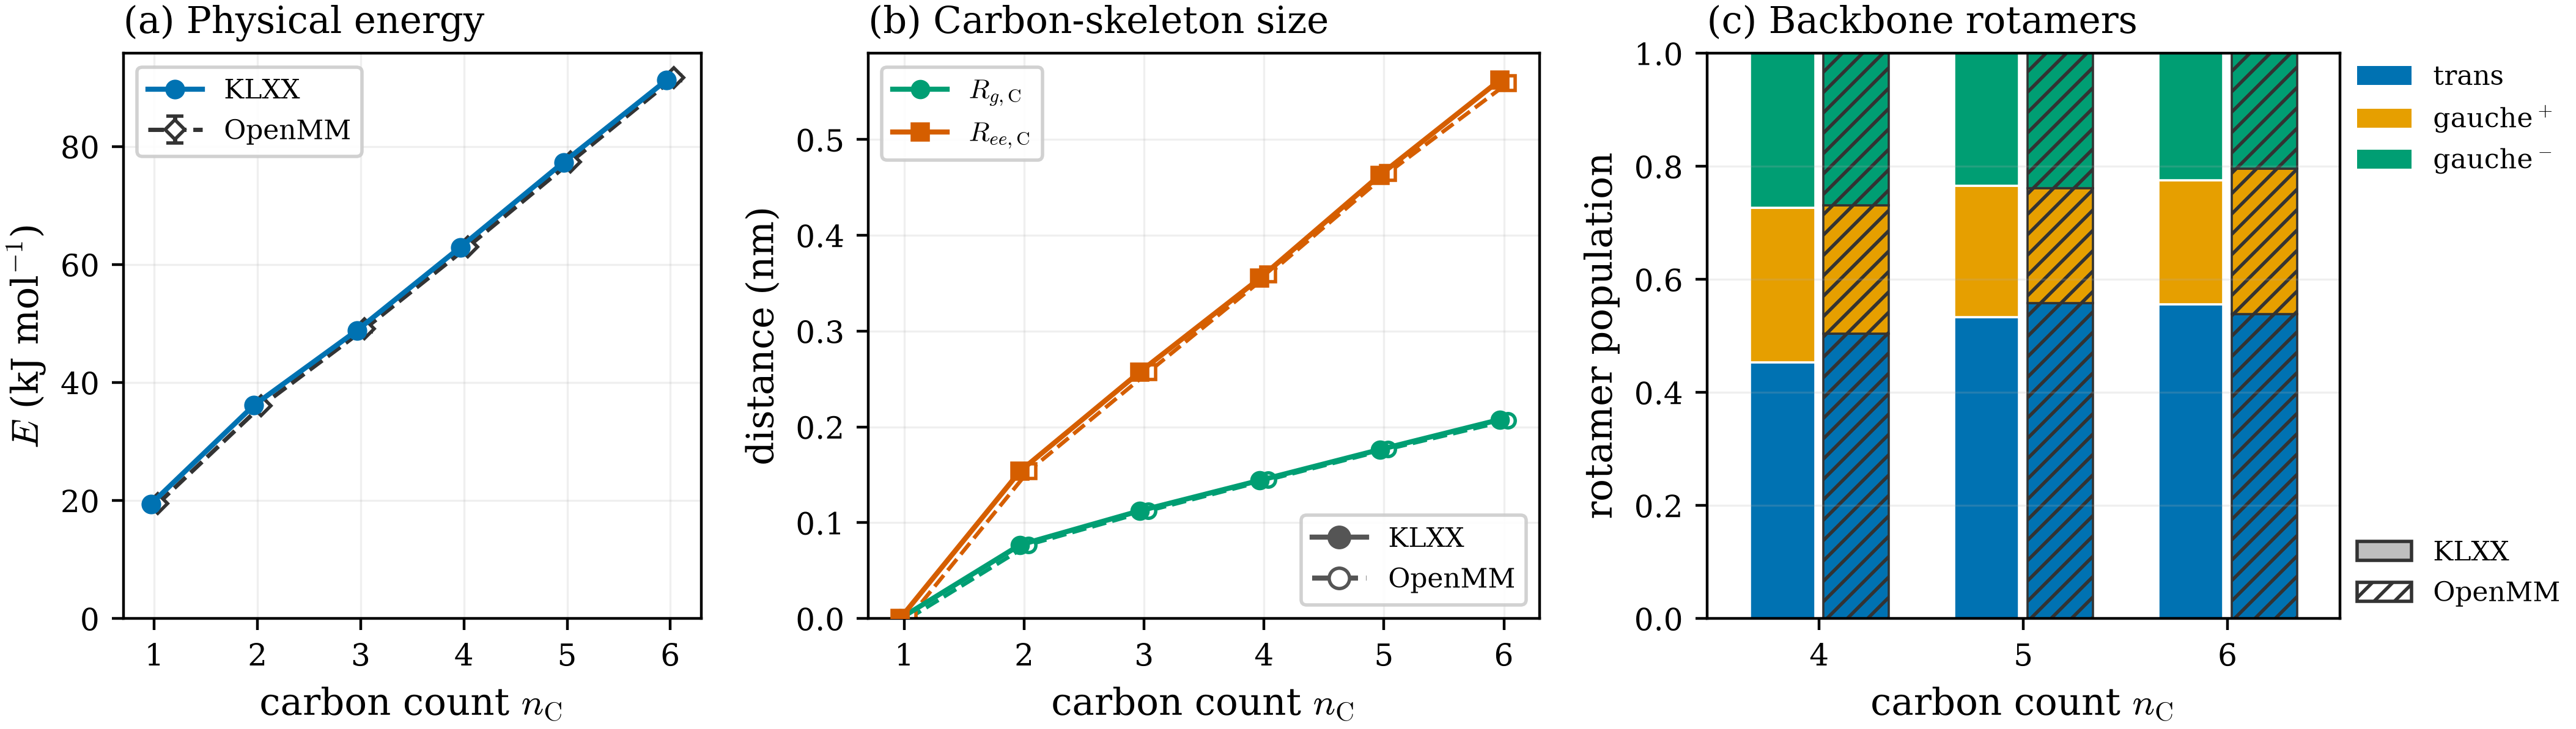
\includegraphics[width=\textwidth]{figures/molecular_alkane_family_macroscopic.png}
\caption{Macroscopic observables from the smallest-factor KLXX sample set for each alkane and an independent physical-potential reference. Fixed-path KLXX is used for methane through propane and sharpening KLXX for butane through hexane. (a) Physical energy evaluated under the exact, unregularized potential. (b) Carbon-skeleton radius of gyration \(R_{g,\mathrm C}\) and terminal-carbon distance \(R_{ee,\mathrm C}\). (c) Pooled backbone trans and gauche fractions. Filled solid curves and unhatched bars denote KLXX; open dashed curves and hatched bars denote the reference.}
\label{fig: alkane-macroscopic}
\end{figure}

The KLXX curves  of Figure~\ref{fig: alkane-macroscopic} are unweighted summaries of the finite-endpoint sample sets; the physical energy $E$ is evaluated only as an observable, without endpoint-to-physical resampling. The physical-potential reference uses two seeds and a $0.25\,\mathrm{fs}$ timestep. Methane through propane use $300\,\mathrm K$ Langevin trajectories; butane through hexane use $300$--$800\,\mathrm K$ PT to mix the backbone rotamers. Across the six molecules, the maximum relative difference between KLXX and reference physical-energy means is $0.644\%$. The largest relative difference among the nonzero carbon radius-of-gyration and terminal-distance means is $1.058\%$, and the largest absolute rotamer-fraction difference is $0.051$. These results show agreement for the selected energy, size, and rotamer summaries across the \(\mathrm C_1\)--\(\mathrm C_6\) series. 

All thirty identity, forward KL, and KLXX runs in Table~\ref{tab: alkane-summary} are complete, and each configuration has one training seed. The reference frames are correlated, and the two-seed ranges are descriptive rather than framewise confidence intervals. The table therefore compares the recorded runs.


\subsection{Additional achiral molecule results}
\label{sec: mol-achiral-results}

We next test NMA, glycerol, and neutral diethanolamine. Each method uses one seed, a sample set of size \(N=200000\), and batch size \(B=10000\). The flow, SMC, MALA, and QT settings match the larger-alkane configuration above. NMA and glycerol use \(400\) Adam steps per accepted flow stage, while neutral diethanolamine uses \(300\). The three sharpening paths are listed in Table~\ref{tab: mol-achiral-summary}. The two losses use method-specific adaptive stage schedules, so the stage counts and recorded wall times are descriptive rather than fixed-compute comparisons.

\begin{table}[htb]
\centering
\small
\setlength{\tabcolsep}{3.5pt}
\begin{tabular}{lcccccccc}
\toprule
\multirow{2}{*}{molecule (\(d\))} &
\multirow{2}{*}{start \(\rho_0\)} &
\multirow{2}{*}{end \(\rho_1\)} &
\multicolumn{3}{c}{$\KL$+$\X_\pi$} &
\multicolumn{3}{c}{$\KL$+$\X_\pi$+$\X_{(\hat\pi+\bar\nu)/2}$} \\
\cmidrule(lr){4-6}\cmidrule(l){7-9}
& & & \(\hat F_\Sigma\) & stages & time
  & \(\hat F_\Sigma\) & stages & time \\
\midrule
NMA (30) & \((50,0.20)\) & \((100,0.15)\)
& 20.19 & 6 & 6.0 & \(\mathbf{15.12}\) & 5 & 12.1 \\
\addlinespace
glycerol (36) & \((50,0.20)\) & \((100,0.10)\)
& 146.2 & 9 & 16.5 & \(\mathbf{54.16}\) & 8 & 35.8 \\
\addlinespace
neutral diethanolamine (48) & \((50,0.20)\) & \((100,0.10)\)
& 303.1 & 12 & 23.1 & \(\mathbf{140.9}\) & 9 & 43.1 \\
\bottomrule
\end{tabular}
\caption{Boltzmann generator training results for the additional achiral molecules, including propagation factor \(\hat F_\Sigma\), the number of accepted stages, and total wall time in minutes. The two method groups use the full losses $\KL$+$\X_\pi$ and $\KL$+$\X_\pi$+$\X_{(\hat\pi+\bar\nu)/2}$, respectively. Each row reports one seed and one sharpening path; bold marks the smaller \(\hat F_\Sigma\) for that molecule.}
\label{tab: mol-achiral-summary}
\end{table}


Comparing $\KL$+$\X_\pi$ with KLXX, the latter has the smaller propagation factor for all three molecules. Relative to $\KL$+$\X_\pi$, it reduces \(\hat F_\Sigma\) by factors of \(1.34\), \(2.70\), and \(2.15\) for NMA, glycerol, and neutral diethanolamine, respectively, and reaches \(t=1\) in fewer accepted stages in every case. The corresponding KLXX runs require \(2.02\), {\color{purple}\(2.17\)}, and {\color{purple}\(1.87\)} times the recorded wall time. Thus the factor reduction is accompanied by the additional QT and optimization work in KLXX. {\color{blue}The reduction is a statement about the schedule, and it costs nothing in accuracy: Figure~\ref{fig: mol-achiral-dihedrals} plots both losses against the OpenMM PT references, and both track them on the reported marginals.}

Figure~\ref{fig: mol-achiral-stage-ess} resolves each factor into its accepted-stage contributions. Because the two losses use method-specific adaptive stage schedules, the individual arcs are descriptive rather than transition-matched comparisons. Sharpening can have the smaller ESS at intermediate stages, so the total factor includes both ESS values reported on each arc.

\begin{figure}[p]
\centering
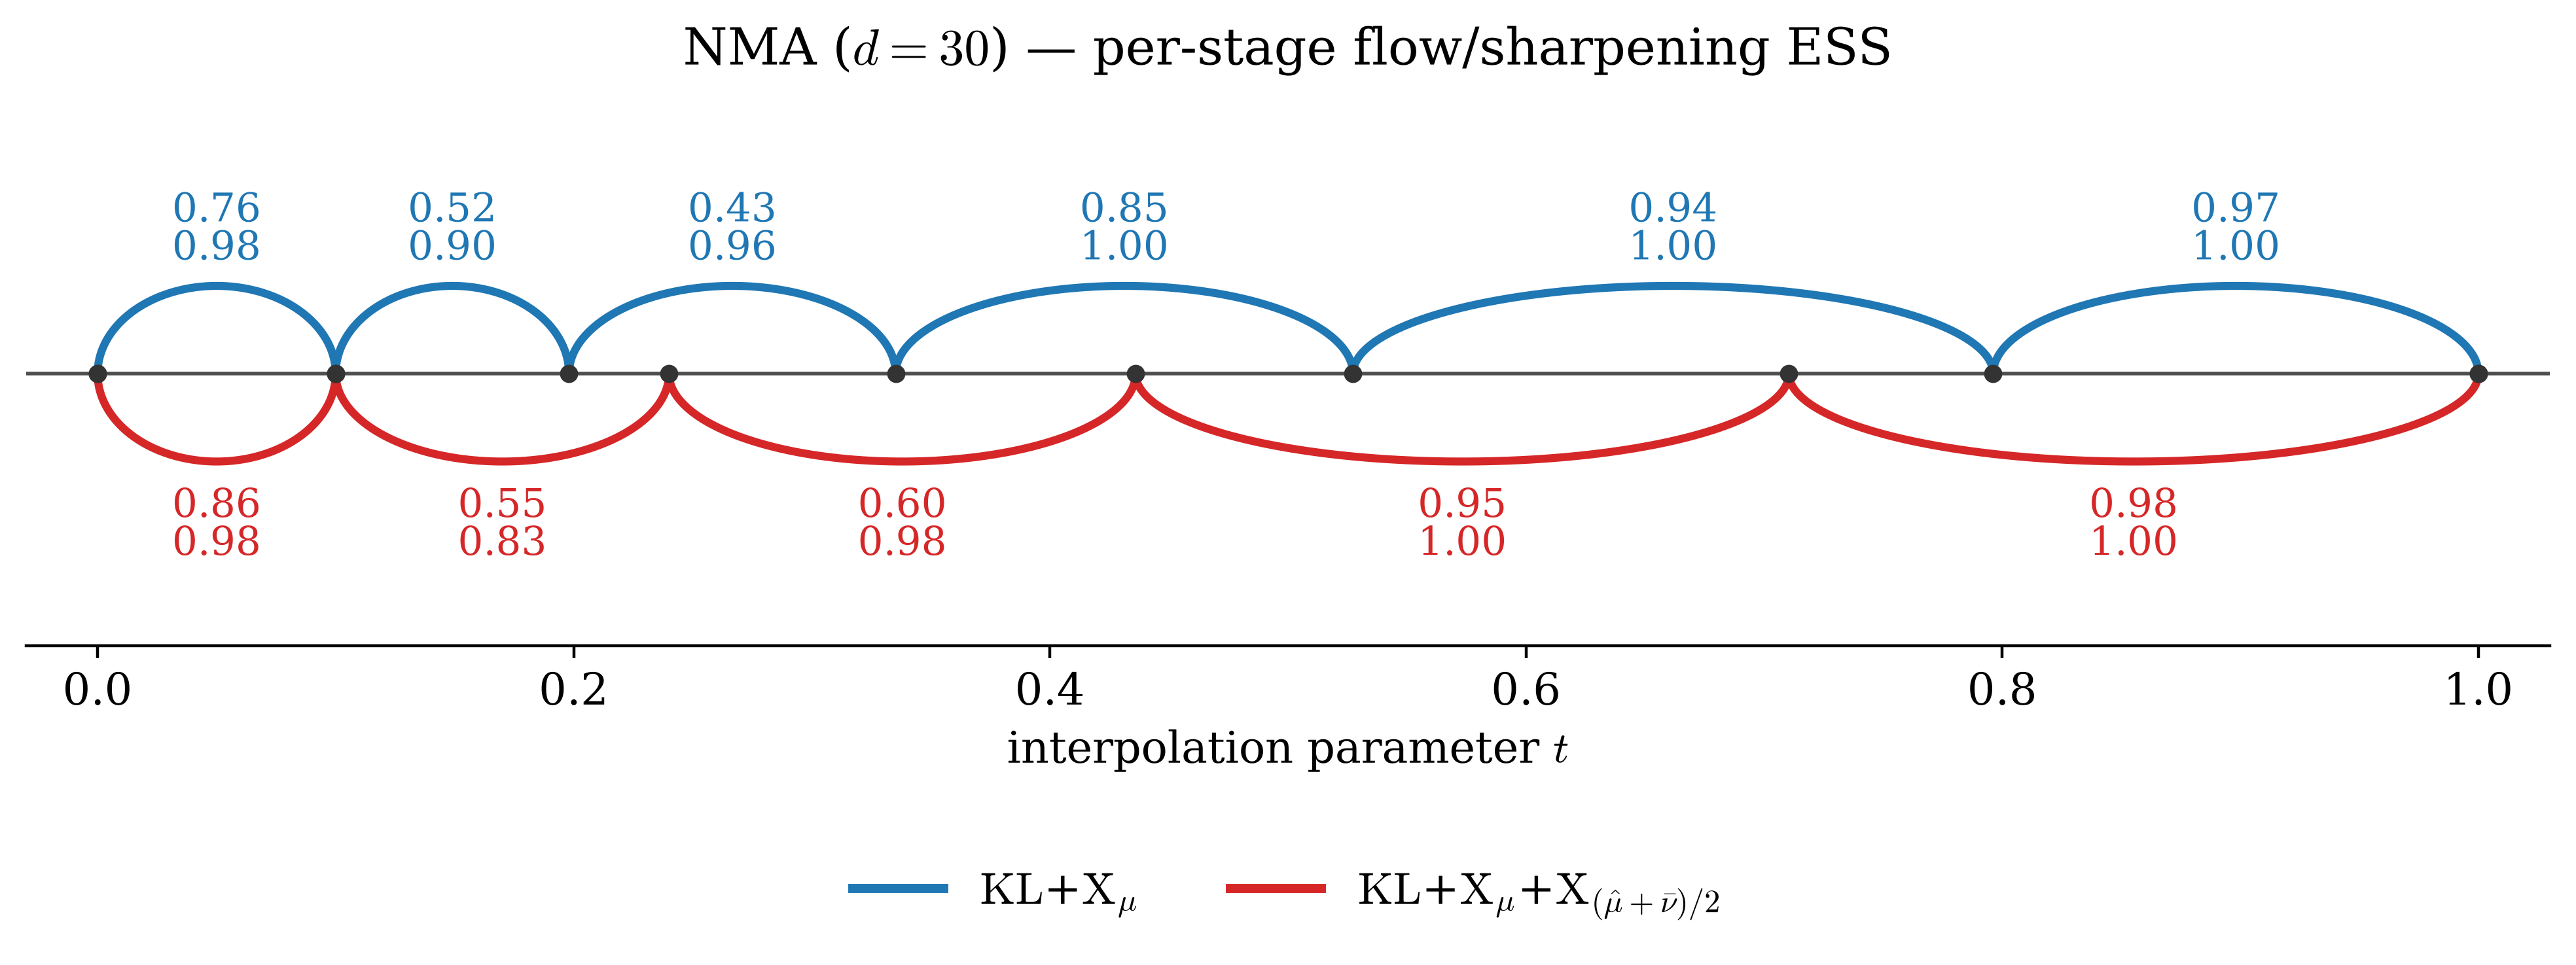
\includegraphics[width=\textwidth]{figures/molecular_nma_30d_stage_ess.png}
\par\smallskip
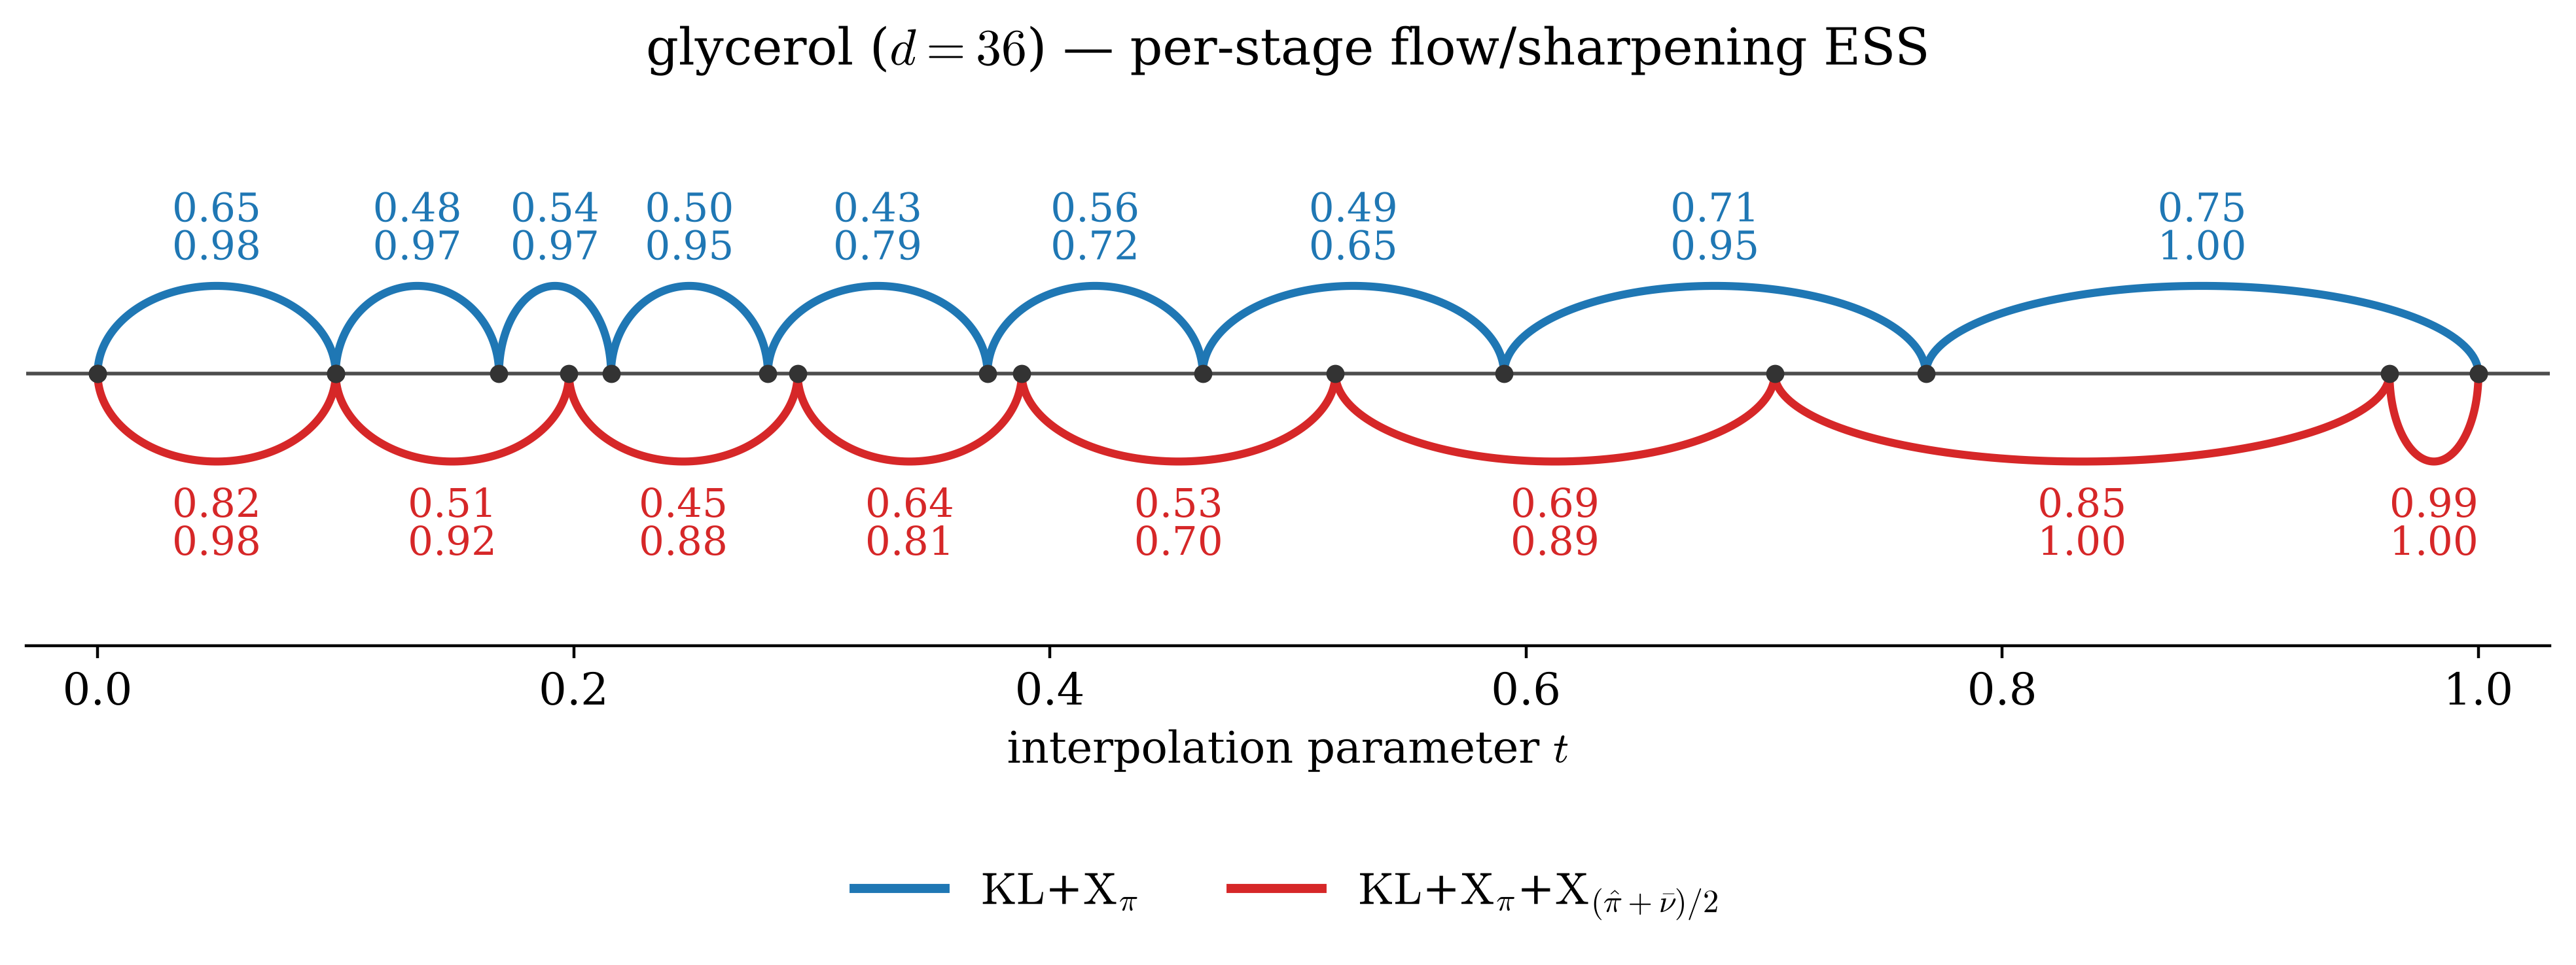
\includegraphics[width=\textwidth]{figures/molecular_glycerol_36d_stage_ess.png}
\par\smallskip
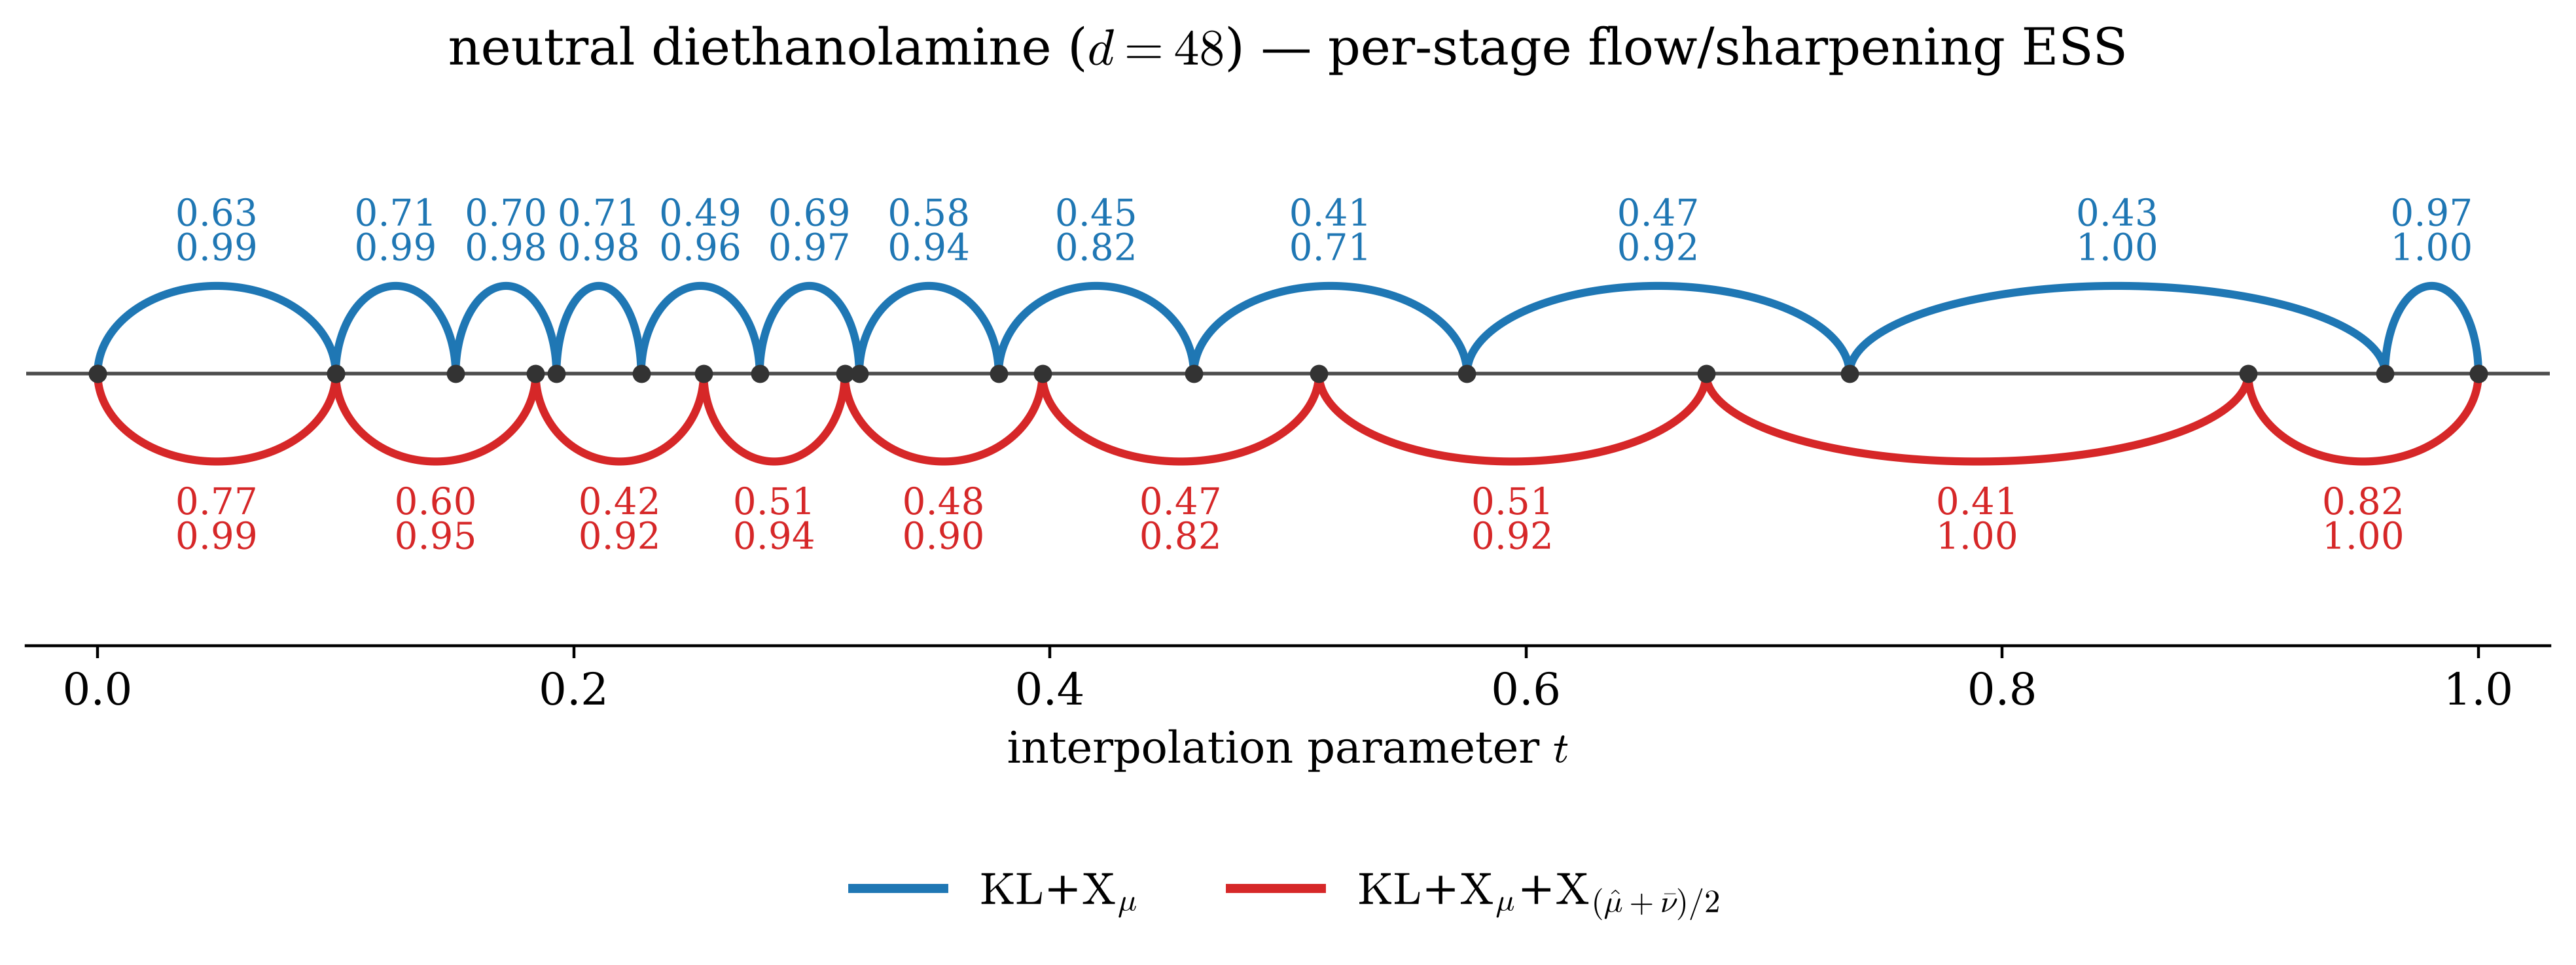
\includegraphics[width=\textwidth]{figures/molecular_diethanolamine_48d_stage_ess.png}
\caption{Per-stage flow and sharpening ESS for NMA (top), glycerol (middle), and neutral diethanolamine (bottom). Each arc spans one accepted transition \(t_{k-1}\to t_k\). Within each stacked annotation, the first row is flow ESS and the second row is sharpening ESS. Blue upper arcs show $\KL$+$\X_\pi$; red lower arcs show $\KL$+$\X_\pi$+$\X_{(\hat\pi+\bar\nu)/2}$. The horizontal coordinate is the source-to-target interpolation parameter \(t\in[0,1]\).}
\label{fig: mol-achiral-stage-ess}
\end{figure}


The final regularized samples are compared with OpenMM PT references, taken at \(300\,\mathrm K\), in Figure~\ref{fig: mol-achiral-dihedrals}. The dashed blue curves are plotted above the solid red curves so that close agreement between samples from the two losses remains visible. The selected torsions resolve the NMA amide trans basin and the trans/gauche wells of glycerol and neutral diethanolamine.

\begin{figure}[htb]
\centering
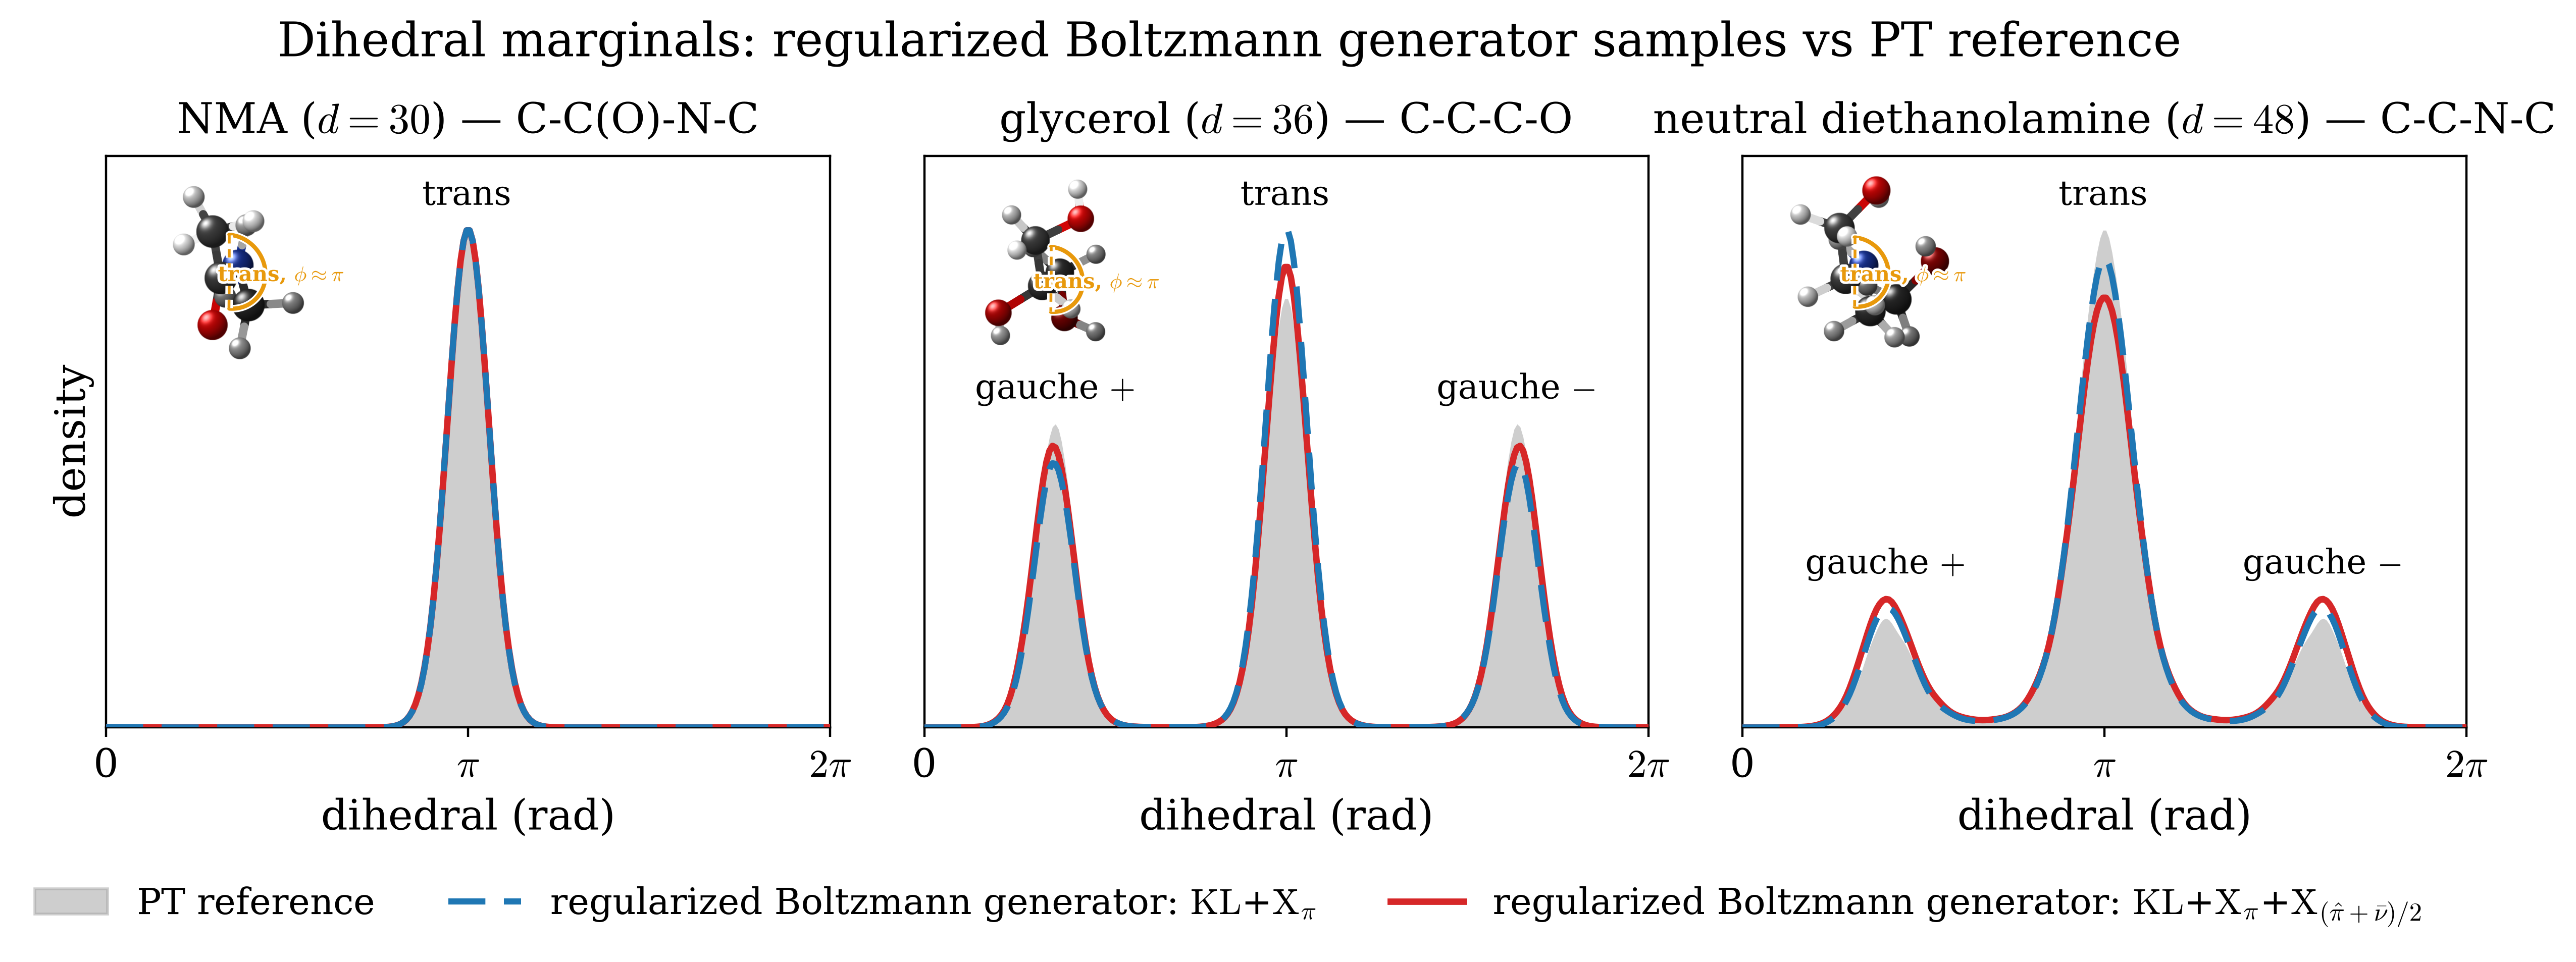
\includegraphics[width=\textwidth]{figures/molecular_achiral_dihedrals.png}
\caption{Selected dihedral marginals from regularized Boltzmann generator samples and OpenMM PT references for NMA, glycerol, and neutral diethanolamine. Gray denotes the reference; dashed blue denotes $\KL$+$\X_\pi$, and solid red denotes $\KL$+$\X_\pi$+$\X_{(\hat\pi+\bar\nu)/2}$. The upper-left insets show representative trans conformers. The NMA reference is a PT trajectory initialized in the trans basin, whereas the glycerol and neutral diethanolamine references pool two seeds. The NMA panel is therefore a trans-basin comparison rather than an estimate of the equilibrium cis/trans populations.}
\label{fig: mol-achiral-dihedrals}
\end{figure}

The curves overlap closely on these selected one-dimensional marginals. The reference frames are correlated, and every generator configuration has one training seed.


\subsection{Chiral molecule results}
\label{sec: mol-chiral-results}

\paragraph{Molecular setup.}
We report runs for alanine dipeptide in its \(\mathrm L\) form, \((2R,3R)\)-2,3-butanediol, and Ac-Pro-NHMe. Only the KLXX loss is evaluated. Every run uses seed \(0\), \(250\) Adam steps per accepted flow stage, an \(8\)-level SMC ladder, and \(100\) mixed-domain MALA steps. The sample set and batch size pairs are \(3.0\times10^5/1.5\times10^4\), \(2.4\times10^5/1.2\times10^4\), and \(3.2\times10^5/1.6\times10^4\), respectively. After training, each stage flow is replayed on a larger particle set, giving \(10^7\) inference samples for alanine dipeptide and 2,3-butanediol and \(1.5\times10^7\) for Ac-Pro-NHMe. The surfaces below use those inference sets, on which the endpoint-to-physical weights are nearly uniform, with \(\operatorname{RESS}\) equal to \(1.000000\), \(0.999981\), and \(1.000000\), respectively, so the regularized endpoint and the physical potential are indistinguishable on the sampled region.

Training never carries more than \(3.2\times10^5\) samples, which keeps the wall times of Table~\ref{tab: mol-chiral-summary} modest. The inference sets are produced afterwards by replaying frozen flows without backpropagation. Replay evaluates the NSF inverse \(G^{-1}\), the expensive direction for this flow structure, and consists of independent map evaluations. The training schedule is sequential in the stage index, and the reference simulations of Section~\ref{sec: alkane-results} advance their trajectories sequentially in time.

\begin{table}[htb]
\centering
\small
\setlength{\tabcolsep}{5pt}
\begin{tabular}{lccccc}
\toprule
\multirow{2}{*}{molecule (\(d\))} &
\multirow{2}{*}{start \(\rho_0\)} &
\multirow{2}{*}{end \(\rho_1\)} &
\multicolumn{3}{c}{$\KL$+$\X_\pi$+$\X_{(\hat\pi+\bar\nu)/2}$} \\
\cmidrule(l){4-6}
& & & \(\hat F_\Sigma\) & stages & time (min) \\
\midrule
alanine dipeptide (60)
& \((50,0.25)\) & \((125,0.10)\) & 68.08 & 10 & 72.7 \\
\addlinespace
\((2R,3R)\)-2,3-butanediol (42)
& \((50,0.20)\) & \((100,0.10)\) & 37.45 & 8 & 35.8 \\
\addlinespace
Ac-Pro-NHMe (72)
& \((50,0.25)\) & \((150,0.10)\) & 176.7 & 11 & 124.7 \\
\bottomrule
\end{tabular}
\caption{Boltzmann generator results for the chiral molecules, including propagation factor \(\hat F_\Sigma\), the number of accepted stages, and total stage time in minutes. The method uses the loss $\KL$+$\X_\pi$+$\X_{(\hat\pi+\bar\nu)/2}$. Each row reports one seed and one sharpening path.}
\label{tab: mol-chiral-summary}
\end{table}

All three runs reach \(t=1\); Table~\ref{tab: mol-chiral-summary} gives their sharpening paths and stage summaries. The propagation factor is accumulated over the flow and sharpening ESS of every accepted stage, as in the earlier molecular tables. The three rows are different molecules with different sample sizes and regularization paths.

Figure~\ref{fig: mol-chiral-conformations} shows one representative final-stage conformation per target, with gold rings on the fixed stereocenters: the \(S\) alanine \(\mathrm C_\alpha\), both \(R\) centers of 2,3-butanediol, and the \(S\) proline \(\mathrm C_\alpha\).

\begin{figure}[htb]
\centering
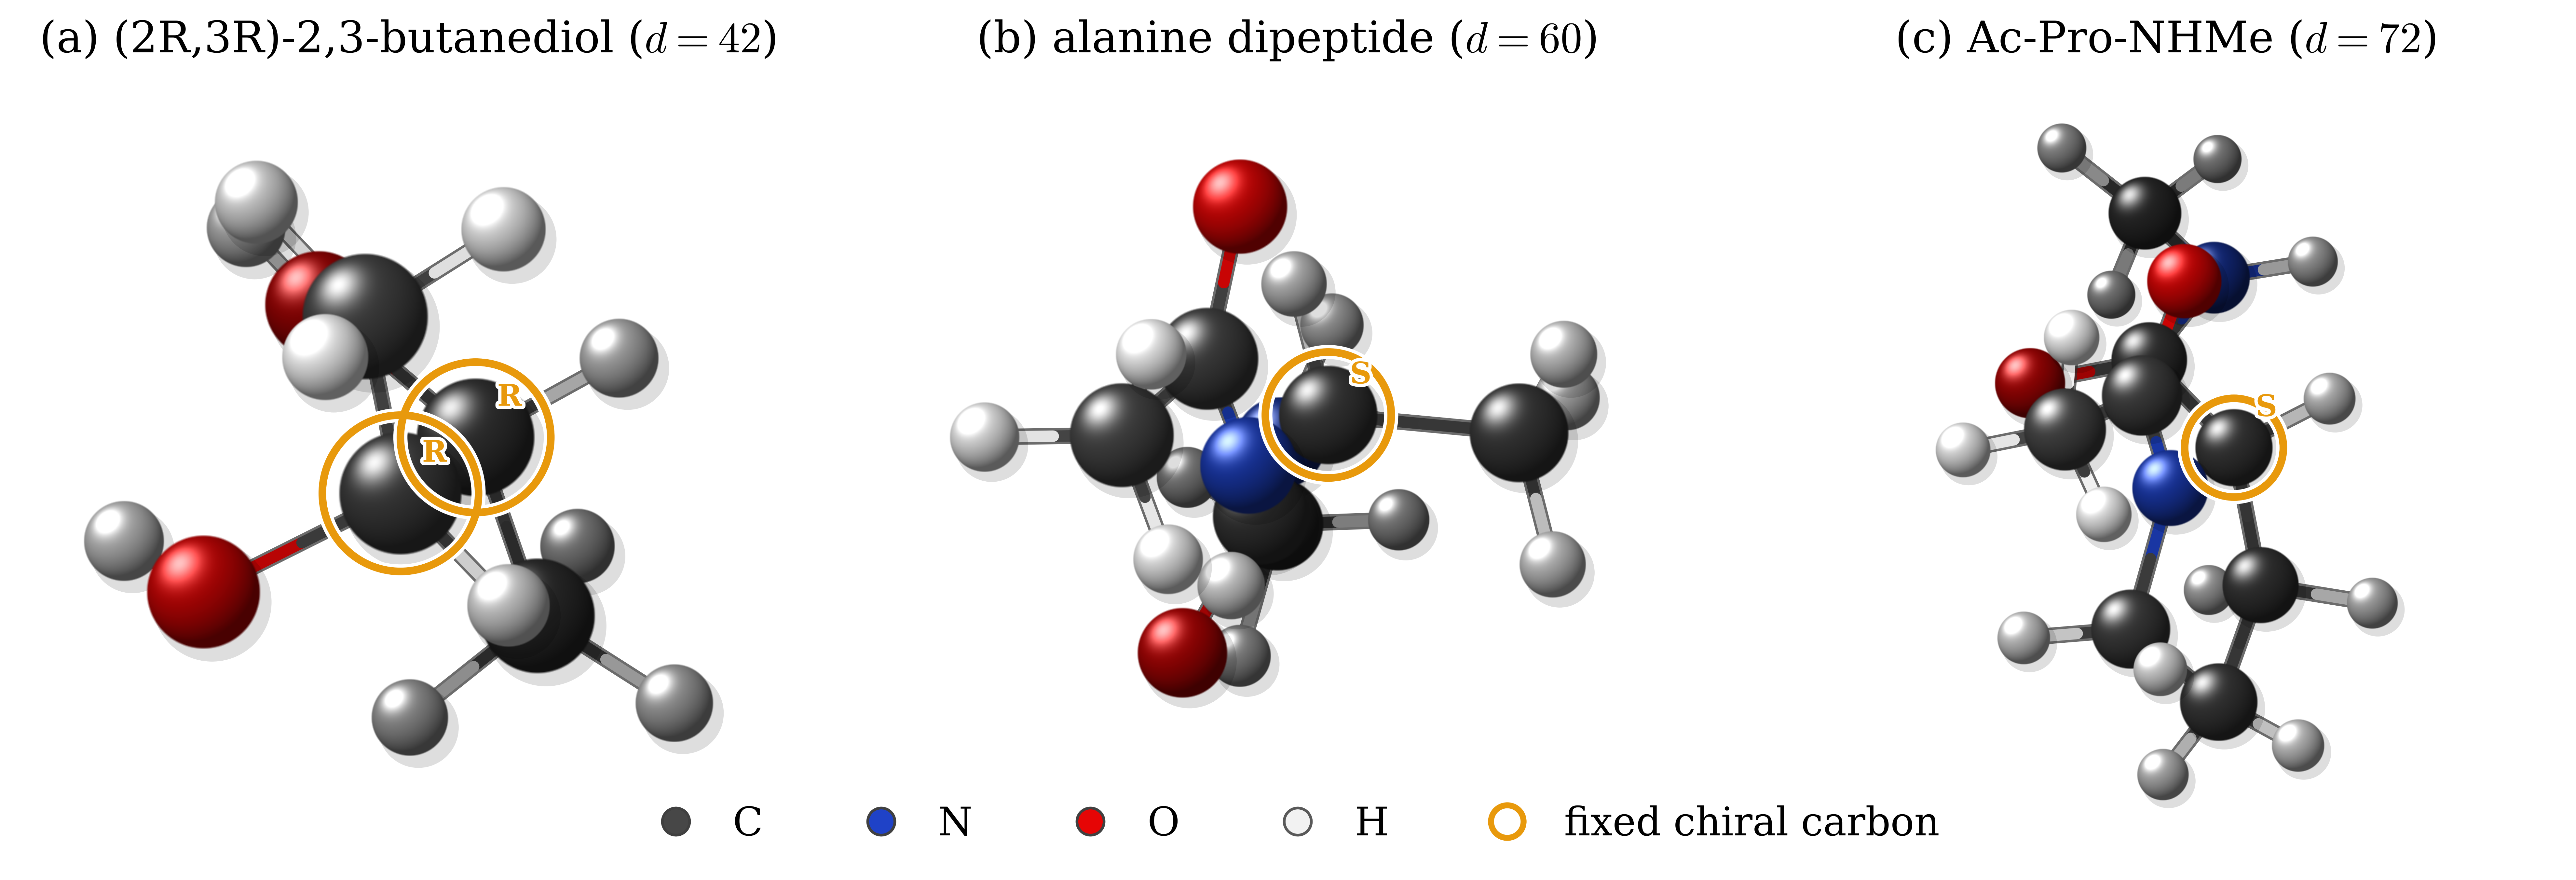
\includegraphics[width=\textwidth]{figures/molecular_chiral_conformations.png}
\caption{Representative final-stage conformations for the three completed chiral targets. From left to right: \(\mathrm L\)-alanine dipeptide, \((2R,3R)\)-2,3-butanediol, and Ac-Pro-NHMe. Gold rings and the adjacent \(R/S\) labels identify every fixed stereocenter; the atom colors follow the CPK convention shown in the legend. Each structure is the sample nearest the modal center of a molecule-specific two-dihedral histogram.}
\label{fig: mol-chiral-conformations}
\end{figure}

All three chiral targets carry an independent equilibrium reference; the first is published and the other two are our own. For alanine dipeptide it is the implicit-solvent trajectory data released with the FAB study \citep{midgley2022flow}, generated for the same Hamiltonian and used here as ground truth, with \(10^7\) samples. For 2,3-butanediol it is a PT run on the unregularized physical potential at \(300\,\mathrm K\), six temperatures on a geometric \(300\)--\(800\,\mathrm K\) grid, retaining \(10^5\) frames over \(50.0\,\mathrm{ns}\) after a discarded \(0.5\,\mathrm{ns}\) equilibration, with mean per-pair exchange probability \(0.529\) and \(2.2\times10^4\) transitions among the three central rotamers. For Ac-Pro-NHMe the ACE-PRO amide barrier is about \(26\,k_{\mathrm B}T\), so neither a plain trajectory nor PT crosses it. Its reference instead adds to the \(300\,\mathrm K\) Langevin dynamics a Metropolis rigid \(\pi\) rotation of the proline side of the amide bond; that move is an involution with unit Jacobian, so the jump is exact and the target is never deformed. It retains \(2\times10^6\) samples over \(501.0\,\mathrm{ns}\) at \(0.2028\) jump acceptance, giving \(4.06\times10^{5}\) accepted cis/trans jumps and a blocking standard error of \(0.0003\) on \(p_{\mathrm{cis}}\).

\paragraph{Results comparison.}
Figure~\ref{fig: mol-adp-ramachandran} tracks the alanine dipeptide Ramachandran surface along four accepted sharpening stages.
Table~\ref{tab: mol-adp-reference} compares the final KLXX stage against ground truth on the same \(100\times100\) grid over \((\phi,\psi)\) with the same smoothing, each surface normalized to its own most populated bin, so only per-method values are quoted. The three populations are raw bin counts on that grid, taken before any smoothing: \(\alpha_{\mathrm L}\) is the half-plane \(\phi>0\), and the bins with \(\phi\Le0\) are split by the sign of \(\psi\) into \(\beta\)/PPII and \(\alpha_{\mathrm R}\). The \(\phi>0\) half-plane is the sparse region of this target. It holds \(0.33\%\) of the ground-truth mass, a factor of about \(240\) below \(\beta\)/PPII, and the KLXX Boltzmann generator places \(0.0031\) of its own mass there against the ground-truth \(0.0033\), so a region of this weight is reproduced at its own scale rather than left empty or overfilled. The three populations differ by at most \(0.0018\), and the mean free energies agree to \(0.03\,k_{\mathrm B}T\) in every band.

\begin{figure}[p]
\centering
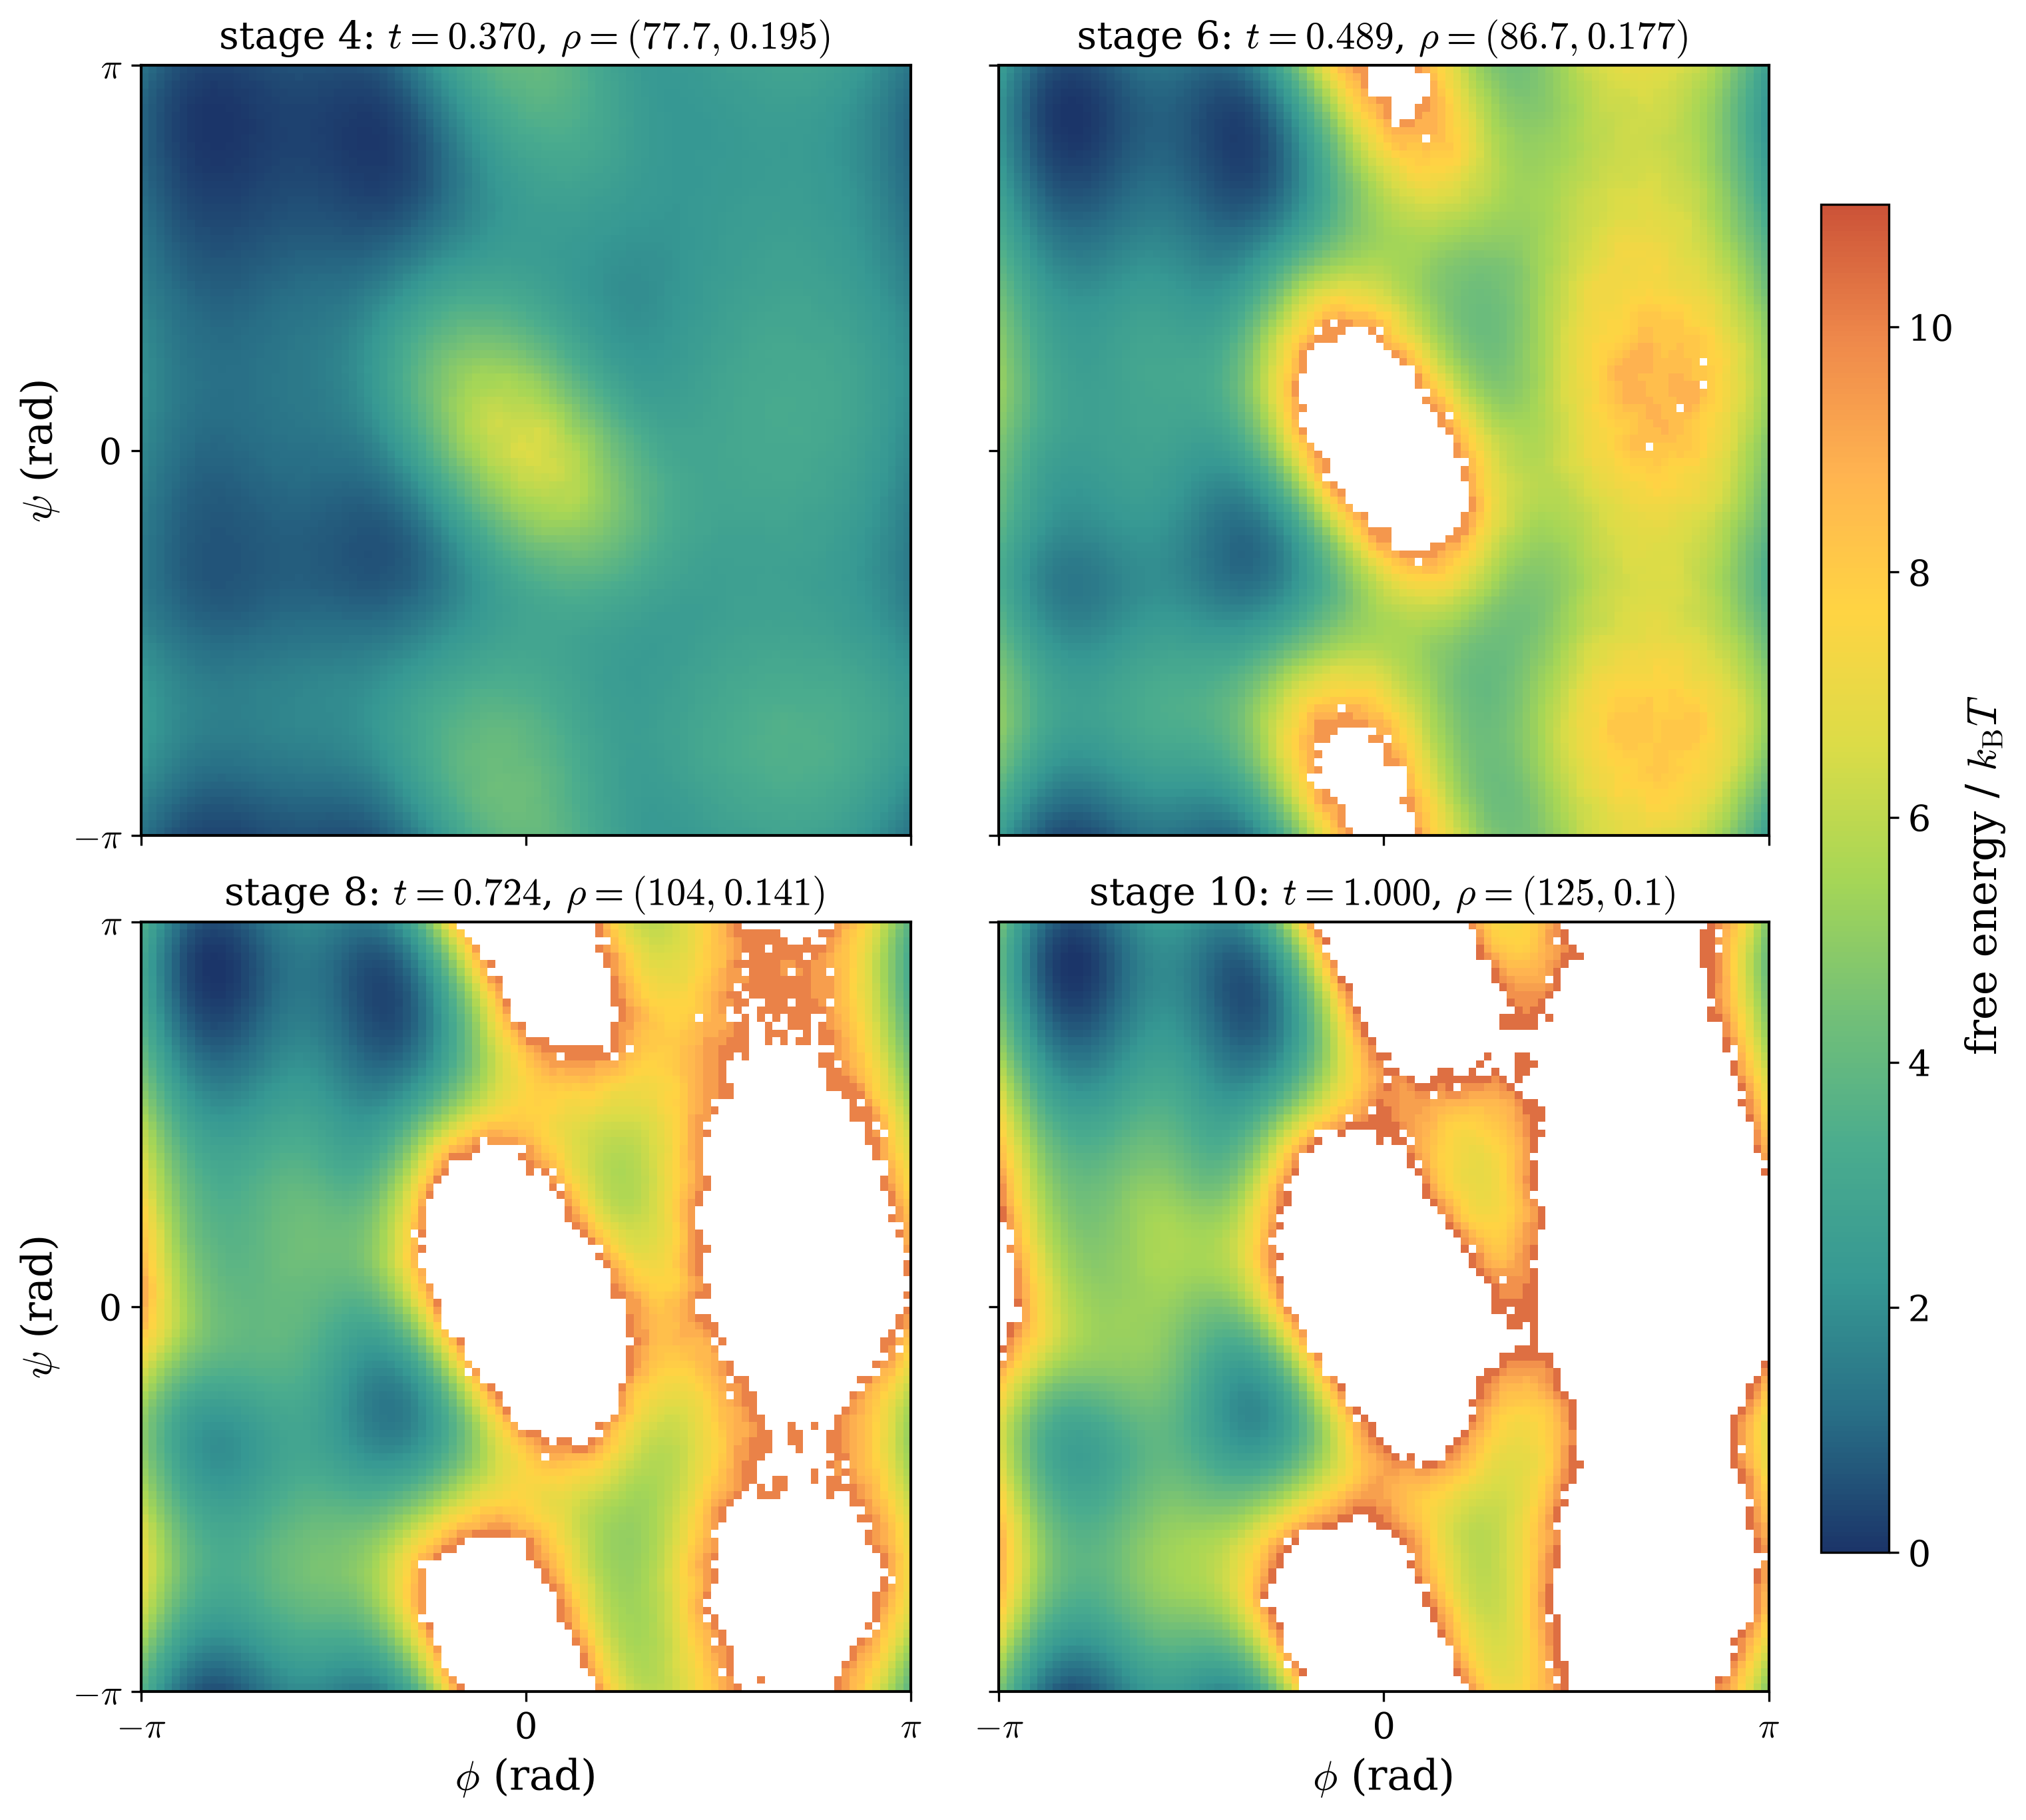
\includegraphics[width=\textwidth]{figures/molecular_adp_ramachandran.png}
\caption{Alanine dipeptide Ramachandran free energy surfaces at accepted stages \(4\), \(6\), \(8\), and \(10\). Each panel contains \(10^7\) inference samples obtained by generating pushforward samples with the corresponding stage flow and then applying resampling, rejuvenation, sharpening, and post-sharpen rejuvenation. The panel titles give the interpolation parameter and regularization value; stage \(10\) reaches \(t=1\) and \(\rho=(125,0.10)\). A common colorbar reports free energy relative to the observed minimum in units of \(k_{\mathrm B}T\).}
\label{fig: mol-adp-ramachandran}
\end{figure}

\begin{table}[htb]
\centering
\small
\begin{tabular}{lccc}
\toprule
& \multicolumn{3}{c}{backbone basin population} \\
\cmidrule(l){2-4}
sample set & \(\alpha_{\mathrm L}\) & \(\beta\)/PPII & \(\alpha_{\mathrm R}\) \\
\midrule
$\KL$+$\X_\pi$+$\X_{(\hat\pi+\bar\nu)/2}$ & 0.0031 & 0.7958 & 0.2012 \\
ground truth & 0.0033 & 0.7940 & 0.2027 \\
\midrule
& \multicolumn{3}{c}{mean free energy by region} \\
\cmidrule(l){2-4}
sample set & low & high & all \\
\midrule
$\KL$+$\X_\pi$+$\X_{(\hat\pi+\bar\nu)/2}$ & 1.230 & 6.323 & 5.379 \\
ground truth & 1.230 & 6.293 & 5.355 \\
\bottomrule
\end{tabular}
\caption{Alanine dipeptide at the final accepted stage against ground truth, the implicit-solvent reference data of \citet{midgley2022flow}, both with \(10^7\) samples. Basins split the \((\phi,\psi)\) plane by \(\phi>0\) for \(\alpha_{\mathrm L}\) and, for \(\phi\Le0\), by the sign of \(\psi\). Bins are classified by the reference surface as low below \(2\,k_{\mathrm B}T\) and high above \(3\,k_{\mathrm B}T\), and restricted to bins finite in both surfaces; entries are mean free energies in units of \(k_{\mathrm B}T\).}
\label{tab: mol-adp-reference}
\end{table}

Figure~\ref{fig: mol-butanediol-landscape} compares the accepted 2,3-butanediol stage nearest \(t=0.5\) with the final stage; both rows resolve the heavy-atom rotamers and hydroxyl orientations.
Table~\ref{tab: mol-butanediol-reference} compares the final KLXX stage against the 2,3-butanediol reference on the same \(100\times100\) torsion grid with the same smoothing. The two sample sets differ in size by two orders of magnitude, so the two halves of the table are reported at different sample counts. A basin population and a mean over occupied bins are ratios, estimated without bias at either size, so both are quoted from the full \(10^7\) inference set. A maximum free energy is not such a quantity: each surface is normalized to its own most populated bin, so the deepest value it can resolve is set by the bin holding a single sample. Maxima are quoted only at matched count, with the same inference set thinned to the reference's \(10^5\).

\begin{figure}[htb]
\centering
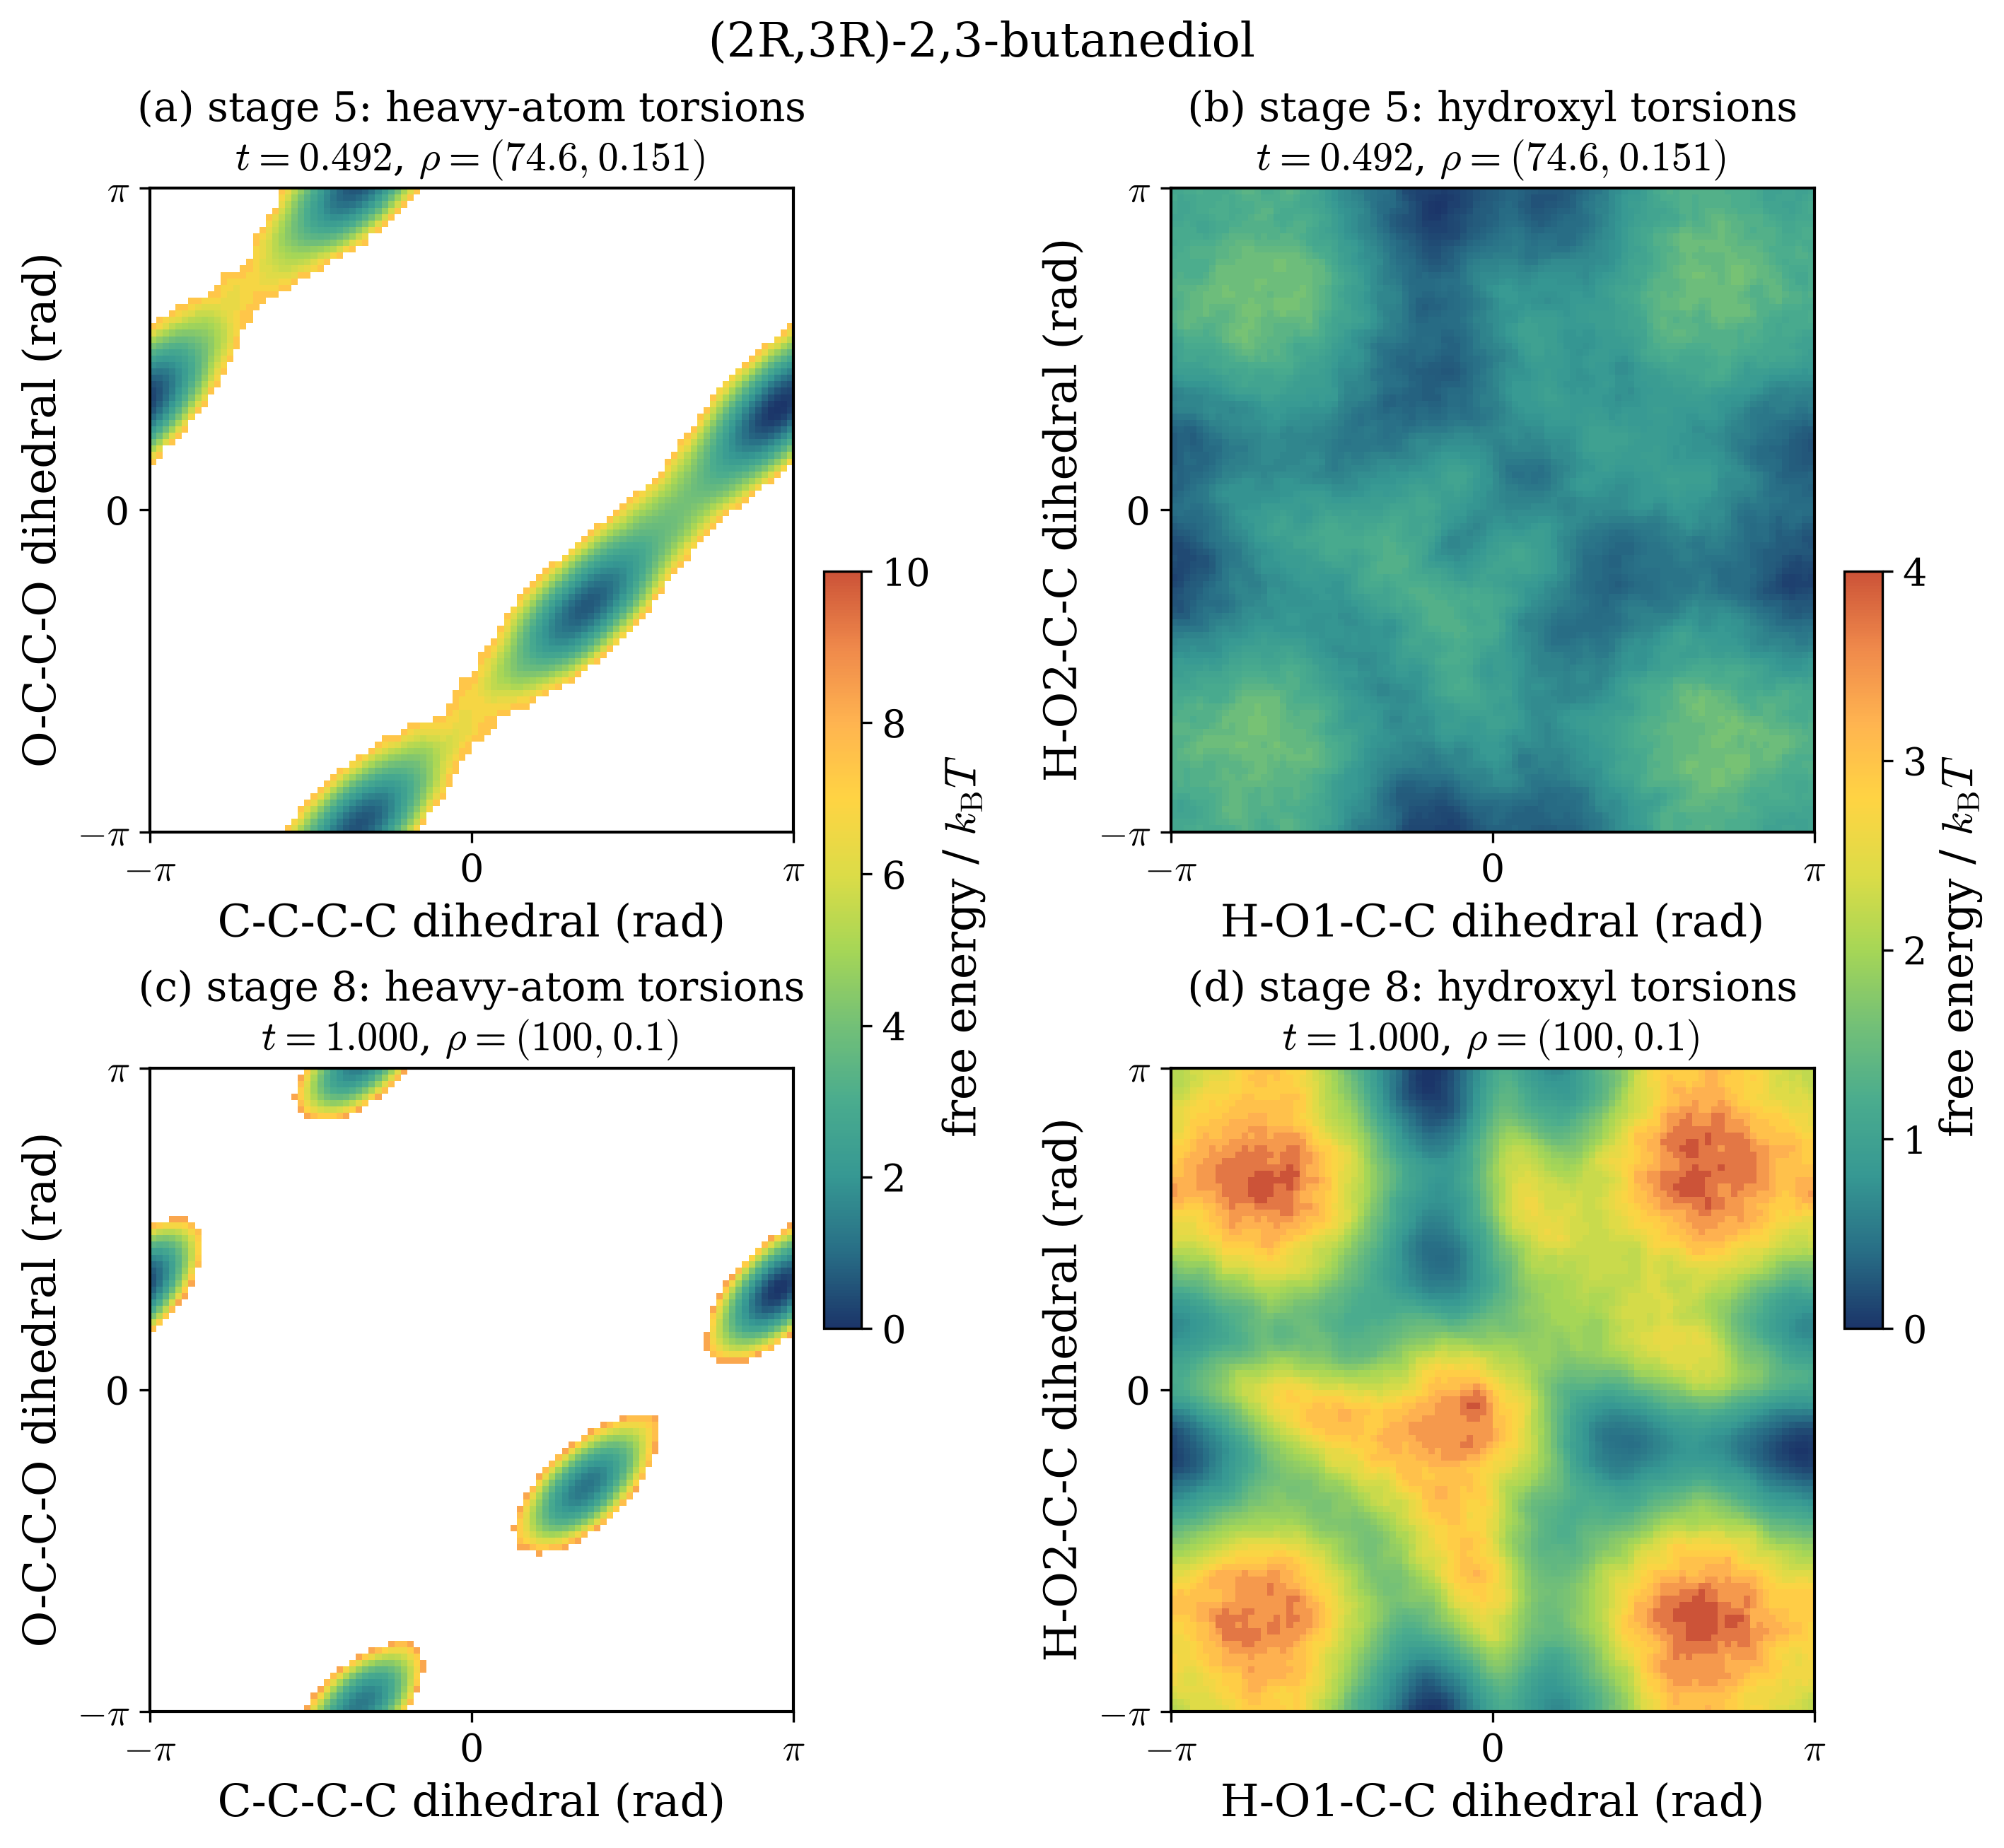
\includegraphics[width=0.88\textwidth]{figures/molecular_rr_2_3_butanediol_landscape.png}
\caption{Conformational free energy surfaces for \((2R,3R)\)-2,3-butanediol from \(10^7\) inference samples per stage. The upper row is stage \(5\), the accepted stage nearest \(t=0.5\), at \(t=0.492\) and \(\rho=(74.6,0.151)\); the lower row is the final stage \(8\) at \(t=1\) and \(\rho=(100,0.10)\). The left column shows the C-C-C-C and O-C-C-O heavy-atom torsions, and the right column shows the two hydroxyl-orientation torsions. Each column shares its scale across stages, and the two diagnostics have separate colorbars in units of \(k_{\mathrm B}T\).}
\label{fig: mol-butanediol-landscape}
\end{figure}

\begin{table}[htb]
\centering
\small
\begin{tabular}{lccc}
\toprule
& \multicolumn{3}{c}{central C-C-C-C rotamer population} \\
\cmidrule(l){2-4}
sample set & gauche\(-\) & gauche\(+\) & trans \\
\midrule
$\KL$+$\X_\pi$+$\X_{(\hat\pi+\bar\nu)/2}$ & 0.1486 & 0.1861 & 0.6652 \\
OpenMM reference & 0.1425 & 0.1726 & 0.6849 \\
\midrule
& \multicolumn{3}{c}{mean free energy by region} \\
\cmidrule(l){2-4}
sample set & low & high & all \\
\midrule
$\KL$+$\X_\pi$+$\X_{(\hat\pi+\bar\nu)/2}$ & 1.229 & 5.126 & 4.137 \\
OpenMM reference & 1.259 & 5.353 & 4.309 \\
\bottomrule
\end{tabular}
\caption{\((2R,3R)\)-2,3-butanediol at the final accepted stage against an independent OpenMM PT reference, with \(10^7\) inference samples and \(10^5\) reference frames. Rotamers split the central C-C-C-C torsion at its eclipsed barriers, trans for \(|\phi|\Ge2\pi/3\) and one gauche well on either side of \(\phi=0\). Bins are classified by the reference surface as low below \(2\,k_{\mathrm B}T\) and high above \(3\,k_{\mathrm B}T\), and restricted to bins finite in both surfaces; entries are mean free energies in units of \(k_{\mathrm B}T\) on the heavy-atom torsions.}
\label{tab: mol-butanediol-reference}
\end{table}

The results of KLXX and the 2,3-butanediol reference agree closely: the rotamer populations differ by at most \(0.020\), in the dominant trans well; the mean free energies on the heavy-atom torsions by at most \(0.23\,k_{\mathrm B}T\); and at matched sample count the maxima by \(0.02\,k_{\mathrm B}T\) on the heavy-atom torsions, \(7.52\) against \(7.54\), and \(0.00\,k_{\mathrm B}T\) on the hydroxyl torsions, \(4.04\) against \(4.04\). The residual trans difference is larger than the reference's own sampling error, which the rotamer transition count places near \(0.003\), so it is not attributable to reference noise alone.

Ac-Pro-NHMe adds a ring degree of freedom and a cis/trans peptide torsion. Figure~\ref{fig: mol-ac-pro-landscape} compares the accepted stage nearest \(t=0.5\) with the final stage.
Table~\ref{tab: mol-ac-pro-reference} compares the final KLXX stage against the Ac-Pro-NHMe reference. The two sets agree on the qualitative picture and disagree quantitatively on the minority sector: both populate cis and trans with trans as the majority, and the two cis-to-trans free energy differences are within \(0.53\,\mathrm{kJ/mol}\) of each other, while the cis populations differ by \(0.0244\).

\begin{figure}[!htb]
\centering
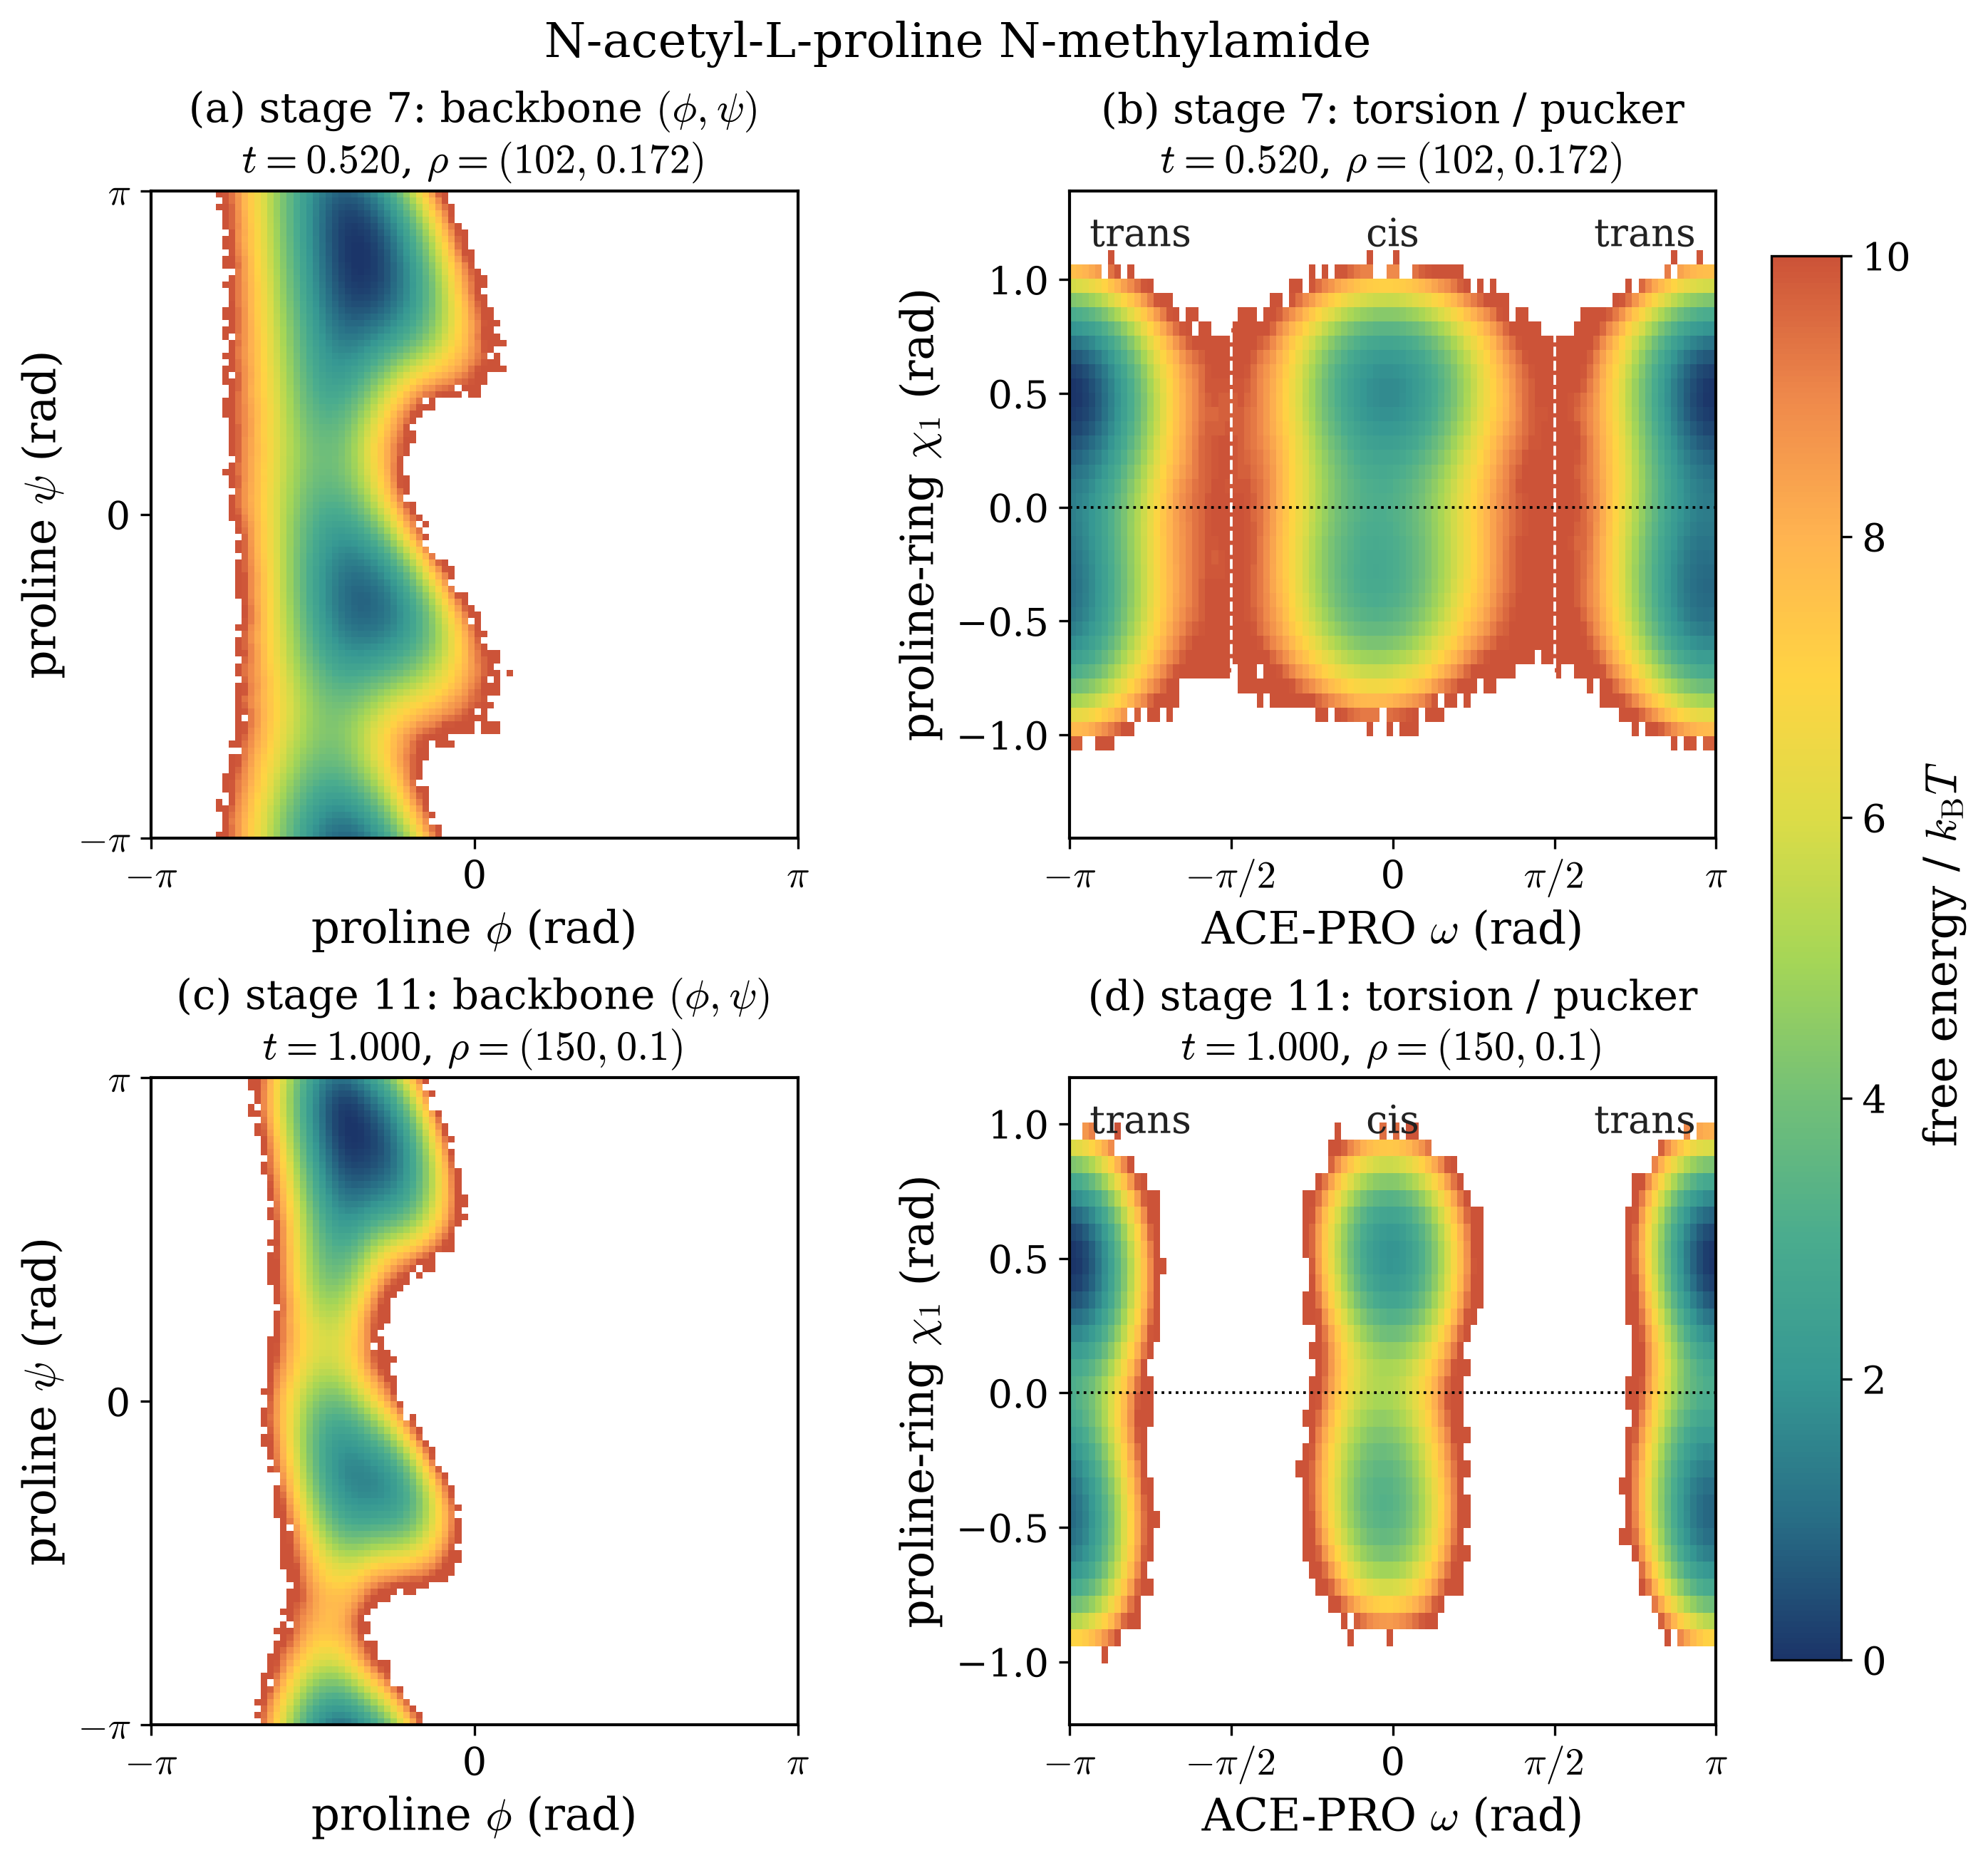
\includegraphics[width=0.95\textwidth]{figures/molecular_ac_pro_nhme_landscape.png}
\caption{Conformational free energy surfaces for Ac-Pro-NHMe from \(1.5\times10^7\) inference samples per stage. The upper row is stage \(7\), the accepted stage nearest \(t=0.5\), at \(t=0.520\) and \(\rho=(102,0.172)\); the lower row is the final stage \(11\) at \(t=1\) and \(\rho=(150,0.10)\). The left column shows the proline backbone \((\phi,\psi)\) surface, and the right column shows the joint ACE-PRO peptide torsion \(\omega\) and proline-ring pucker \(\chi_1\), with the cis and trans sectors marked. All four panels share one free energy scale in units of \(k_{\mathrm B}T\).}
\label{fig: mol-ac-pro-landscape}
\end{figure}

\begin{table}[htb]
\centering
\small
\begin{tabular}{lccc}
\toprule
sample set & cis & trans & free energy \\
\midrule
$\KL$+$\X_\pi$+$\X_{(\hat\pi+\bar\nu)/2}$ & 0.1199 & 0.8801 & 4.97 \\
OpenMM reference & 0.1443 & 0.8557 & 4.44 \\
\bottomrule
\end{tabular}
\caption{Ac-Pro-NHMe peptide torsion populations at the final accepted stage against an independent OpenMM reference, with \(1.5\times10^7\) inference samples and \(2\times10^6\) reference samples. Cis is \(|\omega|<\pi/2\), counted per sample on both sides. Free energy differences are cis minus trans, in kJ/mol.}
\label{tab: mol-ac-pro-reference}
\end{table}

\paragraph{Ac-Pro-NHMe residual gap.}
Ac-Pro-NHMe is the most difficult of the three chiral targets: its two peptide sectors are separated by the ACE-PRO amide barrier of about \(26\,k_{\mathrm B}T\), which neither Langevin dynamics nor PT crosses, and even the reference needs a Metropolis rigid \(\pi\) rotation of the proline side of that bond before it can equilibrate the two sectors. The KLXX Boltzmann generator uses no reference frames, no bias potential, no elevated temperature, and no conformational prior, yet it populates both peptide sectors, keeps the \(S\) proline \(\mathrm C_\alpha\), and orders the sectors correctly.

The residual gap is consistent with a finite sample rather than with a systematic error in the method. By Theorem~\ref{thm: propagation}, {\color{blue}the inference scheme of Algorithm~\ref{alg: inference}} is asymptotically unbiased whenever the stage weight suprema are finite, so a discrepancy that survives at fixed \(N\) is the finite-sample term and should shrink as \(N\) grows. {\color{purple}Read at $\operatorname{osc}(\varphi)=1$, the scale $\hat F_\Sigma/(2\sqrt N)$ is \(0.011\), \(0.006\), and \(0.023\) for alanine dipeptide, 2,3-butanediol, and Ac-Pro-NHMe. The alanine dipeptide gap of \(0.002\) sits below its scale and the Ac-Pro-NHMe gap of \(0.024\) sits at its scale; the 2,3-butanediol rotamer gap of \(0.020\) sits above its own, so that residual is left open. Since $\hat F_\Sigma$ is not a bound, none of the three readings is decisive.} The near-singular core of the potential explains the residual gap more plausibly than the higher dimension of Ac-Pro-NHMe.

The direct test is a larger inference set, which we do not run: the replay cost grows in proportion to the sample count and this target is already the most expensive of the three, so resolving a difference of \(0.02\) in a population of \(0.14\) is beyond the budget of this study. We leave the gap open rather than close it by tuning.


\subsection{{\color{blue}Discussion on other Boltzmann generator approaches}}
\label{subsec: mol-discussion}

{\color{blue}The published ESS values for alanine dipeptide are those of a single flow against the target: \(92.8\%\) for FAB with its replay buffer in Table~2 of \citet{midgley2022flow}, and \(94.81\%\) when FAB is retrained in an independent study \citep{schopmans2025temperature}, both computed on flow samples after clipping the highest \(0.01\%\) of the importance weights. The staged generator returns a sample set, and reports accordingly: Theorem~\ref{thm: propagation} bounds the error of the inference scheme of Algorithm~\ref{alg: inference} at rate \(N^{-1/2}\) for every bounded observable, provided each stage weight is $\nu_k$-essentially bounded, and the propagation factor $\hat F_\Sigma$ of Table~\ref{tab: mol-chiral-summary} is a computable substitute for the constant of that bound rather than a bound on that constant. The ESS values behind that factor are stagewise, and none of them compares a single flow with $\pi$. The stage count beside that factor is likewise not a count of annealing performed, and what separates the two constructions is what their annealing carries: the MCMC transitions of FAB target $\pi^2/\nu$ and so carry the gradient of the pushforward density, and FAB reuses the samples they produce through a prioritized replay buffer, whereas every MALA chain here targets the current stage target and uses only the potential gradient, and the training keeps no replay buffer, as Section~\ref{subsec: annealing} describes.}

{\color{blue}An ESS of pushforward samples measures uniform observed weights on the support the flow reaches, and a target mode absent from the sample cannot lower it (Section~\ref{subsec: eval}). On alanine dipeptide this limitation is quantitative: the \(\phi>0\) half-plane carries \(0.33\%\) of the ground-truth mass, so a flow that reaches no configuration there contributes no term to \eqref{eq: ESS} from that region, and the normalized ESS returns the same value it would have taken had the target carried no mass there at all. This is how the fake ESS of Section~\ref{subsec: phi4} would arise on a molecular target.}

{\color{blue}Both studies above say the same of an ESS computed on flow samples. \citet{midgley2022flow} write that the ESS of the baselines missing modes is spurious for that reason, and their Table~2 shows the size of the effect: the reverse KL flow reports \(54\%\) against \(2.8\%\) for the flow trained by maximum likelihood on molecular dynamics data, while the reverse KL flow's Ramachandran KL divergence, before reweighting, is worse by more than two orders of magnitude. The TA-BG study \citep{schopmans2025temperature} states that it reports the ESS on flow samples even though that quantity does not capture mode collapse, and in its Table~1 the reverse KL run has the highest ESS of the four methods compared on both alanine tetrapeptide and alanine hexapeptide while collapsing almost entirely onto the main mode.}

{\color{blue}The tables above report what an ESS cannot see: Table~\ref{tab: mol-adp-reference} places \(0.0031\) of the KLXX Boltzmann generator's mass in the \(\phi>0\) half-plane against \(0.0033\) on the reference data of \citet{midgley2022flow}. The training budget behind that agreement is allocated by stage. Each stage advances the interpolation parameter, initializes its flow at the identity, and uses \(250\) Adam steps at a batch size of \(1.5\times10^4\) here, and what carries information from one stage to the next is the sample set rather than the optimizer state. The ten accepted training stages complete in \(72.7\) minutes on one GPU.}

{\color{blue}These runs are offered as evidence for mode coverage rather than as a claim of accuracy across every test. The mixture variation supplies that coverage: its QT set is constructed explicitly, so the candidate modes it finds are placed in the loss by construction and the accompanying ESS becomes a diagnostic that coverage supports rather than one taken on trust. As Section~\ref{subsec: loss-related} notes, that mechanism is not tied to this loss; Section~\ref{subsec: 2d-benchmark} compares KLXX with FAB on the 2D targets, where the runs differ only in the objective, and how KLXX compares with FAB and TA-BG on the molecular targets remains to be explored.}


% ===================== Section 7: Conclusions + Acknowledgement =====================
\section{Conclusions}
\label{sec: conclusions}

Forward KL is mass-covering for exact distributions, but its sampled loss sees only the target regions supplied to it. This gap can produce a fake ESS, transfer surrogate error to the flow, and leave target-poor pushforward regions weakly constrained. Log-ratio variation addresses these failures by comparing the exact log-density ratio at pairs of samples. The weighting measure determines which regions are compared: target samples measure log-ratio variation on reached target regions, QT samples discover candidate modes, and pushforward samples expose regions occupied by the pushforward distribution. KLXX combines these log-ratio variations while retaining the exact target as a minimizer and a tractable pushforward density.

The theory covers the generalized KLXX loss at any coefficients $(\lambda,\vartheta,\alpha,\beta)$. In FR geometry the loss induces a gradient flow whose dissipation \eqref{eq: combined-rate} carries both log-ratio variations as nonpositive terms, with no log-concavity, spectral gap, or growth assumption on $\pi$. Under a fixed biased target surrogate, Theorem~\ref{thm: accuracy} subtracts one nonnegative discrepancy for each variation from the stationary error bound, {\color{blue}requiring positive densities and two finite importance-weight expectations}. Theorem~\ref{thm: propagation} is separate: it bounds the $L^2$ error of {\color{blue}the inference scheme of Algorithm~\ref{alg: inference}} at rate $N^{-1/2}$ for every bounded observable, with a constant independent of $N$, so the scheme is asymptotically unbiased{\color{purple}, provided each stage weight is $\nu_k$-essentially bounded}. The reported $\hat F_\Sigma$ summarizes stagewise weight degeneracy and is a computable substitute for that constant rather than a bound on it.

The model problems are consistent with the roles of the target, QT, and pushforward samples. {\color{blue}On Three-Well, Himmelblau and Sparse, forward KL and $\KL$+$\X_\pi$ miss modes while reporting a high ESS, and on the $\phi^4$ lattices they collapse to one well with $\KL$+$\X_\pi$ holding the highest ESS at both sizes; both QT-based losses recover every mode on these targets, and adding the pushforward samples to the mixture reduces the visible intermodal mass on Himmelblau, Sparse and the $L=8$ lattice.} {\color{blue}The product multi-well test shows higher sample ESS than forward KL for every loss with log-ratio variation at all sixteen tested dimensions.} On the shared clock stage schedules, KLXX has higher sample ESS on every shared stage and a smaller propagation factor at every reported batch size. {\color{blue}The $\phi^4$ and clock experiments carry the accuracy evidence, comparing methods on an observable against a known reference value.}

{\color{blue}The molecular summary tables compare schedules, and the reference tables and figures compare samples against independent references.} In the alkane runs, KLXX has the smallest factor in {\color{blue}all ten settings}, while forward KL approaches the identity result as molecule size grows. Sharpening lowers the KLXX factor for the larger alkanes. For NMA, glycerol, and neutral diethanolamine, KLXX also has a smaller factor than $\KL$+$\X_\pi$ and reaches the endpoint in fewer accepted stages. {\color{blue}The three chiral KLXX runs reach \(t=1\) and populate multiple torsional basins, and their representative final-stage conformations retain the specified stereochemical configurations.} The alanine dipeptide sample set {\color{blue}agrees with} the published equilibrium reference of \citet{midgley2022flow} on the {\color{blue}Ramachandran basin populations}, including the sparse \(\phi>0\) half-plane. For Ac-Pro-NHMe, reached with no external data and no conformational prior, the KLXX Boltzmann generator populates both peptide sectors and orders them correctly. Selected alkane observables and achiral dihedral marginals agree with independent physical-potential simulations on the reported diagnostics. {\color{blue}What these molecular results establish is that the KLXX Boltzmann generator reaches the torsional basins and returns samples that agree with independent references at a modest budget; they are not a theorem of universal dominance, a fixed-compute comparison, or a claim of accuracy against every alternative.}

{\color{blue}Every configuration outside the $\phi^4$ tests is a single training realization and requires additional seeds to measure run-to-run variation.} The finite alkane endpoints have nearly uniform endpoint-to-physical weights on the reported sample sets. Among the chiral results, alanine dipeptide is checked against published ground truth, and 2,3-butanediol and Ac-Pro-NHMe against references of our own. The Ac-Pro-NHMe comparison agrees on the qualitative picture and leaves a quantitative gap in the cis population. {\color{blue}Theorem~\ref{thm: propagation} is consistent with reading that gap as a finite-sample term}; resolving it would require an inference set beyond the budget of this study, so we report it open.

{\color{blue}Section~\ref{subsec: mol-discussion} sets these results against the single-flow ESS values that other Boltzmann generators report. The principle those results support is not an ordering of methods: what the mixture variation contributes is a way past mode collapse, and it does so through an explicitly constructed QT set, so the coverage is placed in the loss rather than hoped for, and the accompanying ESS is a diagnostic that coverage supports.} Future work includes tuning the KLXX loss for better performance and testing more challenging cases such as a Lennard--Jones system and distributions on low-dimensional manifolds. {\color{blue}We will also extend the FAB comparison of Section~\ref{subsec: 2d-benchmark} beyond the 2D targets, and add LDR and TA-BG.} 

\section*{Acknowledgments}

\section*{Data Availability}
The normalizing flow computations use the JAX backend through two Python packages maintained by Xuda Ye. The packages \texttt{jflows} and \texttt{jflows-md} can be installed directly from PyPI with:
\begin{tcolorbox}[colback=gray!12,boxrule=0pt,arc=2pt,left=6pt,right=6pt,top=4pt,bottom=4pt]
\texttt{pip install jflows==0.5.4 jflows-md==0.5.4}
\end{tcolorbox}
\noindent
Molecular benchmark data were generated with OpenMM and AmberTools, and the alanine dipeptide reference data were taken from the FAB study \citep{midgley2022flow}. The source files are available at:
\begin{tcolorbox}[colback=gray!12,boxrule=0pt,arc=2pt,left=6pt,right=6pt,top=4pt,bottom=4pt]
\url{https://github.com/xuda-ye-math/KLXX}
\end{tcolorbox}
\noindent
The GPU-accelerated runs used one MSI GeForce RTX 5090 32G Gaming Trio OC with $32$\,GB of VRAM. The card ran at a $600$\,W power
limit with clock offsets of $+250$\,MHz on the core and $+2000$\,MHz on the
memory. All reported wall times correspond to this overclocked
configuration.

\subsection*{Declaration of AI use}
The authors used Claude Opus 5 (Anthropic) to assist with writing and testing the codes. All data and numerical results reported in this paper are generated directly by our Python scripts and are presented without any embellishment. The authors have reviewed all AI-assisted content and take full responsibility for the correctness of the results.

{
	\bibliographystyle{abbrvnat}
	\bibliography{references}
}

\appendix

\section{Proof of Fisher--Rao gradient flow convergence}
\label{sec: appendix-FR}

This appendix derives the Fisher--Rao gradient flow \eqref{eq: FR-flow} of the generalized KLXX loss \eqref{eq: KLXX-general-nu} and proves the dissipation identity \eqref{eq: combined-rate} {\color{blue}stated in Section~\ref{subsec: FR-convergence}}. We view $\nu$ as a generic probability density evolving under a Riemannian metric on the space of densities \citep{ambrosio2008gradient,villani2009optimal} and ask how fast $\nu_t$ approaches the target in $\KL(\pi\|\nu_t)$.
Throughout, we assume the densities are positive and regular enough for differentiation, and that the expectations displayed below are finite.

The FR gradient of a functional $\mathcal F[\nu]$ and the flow it generates are given by
\begin{equation}
    \mathrm{grad}^{\mathrm{FR}}\mathcal F(\nu) = \nu\biggl(\frac{\delta\mathcal F}{\delta\nu} - \mathbb E_{\nu}\Big[\frac{\delta\mathcal F}{\delta\nu}\Big]\biggr),
    \qquad
    \partial_t\nu_t = -\,\mathrm{grad}^{\mathrm{FR}}\mathcal F(\nu_t).
    \label{eq: appendix-FR-gradient}
\end{equation}
The mean subtraction enforces $\int_{\mathbb R^d}\mathrm{grad}^{\mathrm{FR}}\mathcal F\D x = 0$ at unit mass, so the flow preserves probability mass.
In the generalized KLXX loss \eqref{eq: KLXX-general-nu},
the forward KL contributes a local term: its first variation is $\delta\KL(\pi\|\nu)/\delta\nu = -w$, and $\mathbb E_\nu[w] = \int_{\mathbb R^d}\pi\D x = 1$, so \eqref{eq: appendix-FR-gradient} gives
\begin{equation}
    \mathrm{grad}^{\mathrm{FR}}\bigl[\KL(\pi\|\nu)\bigr](x) = \nu(x)-\pi(x).
    \label{eq: appendix-FR-grad-KL}
\end{equation}
The two log-ratio variations are handled at once, because neither weighting distribution is varied and nothing in the calculation uses that the weighting distribution and the target coincide.

\begin{lemma}
\label{lem: appendix-variation}
Let $\omega$ be a weighting distribution that does not depend on $\nu$, and let $S^{\omega}$ be its nonlocal correlation \eqref{eq: FR-S}. Then
\begin{equation}
    \frac{\delta \X_\omega(\pi\|\nu)}{\delta\nu}(x) = -2\,\frac{\omega(x)}{\nu(x)}\,S^{\omega}(x),
    \qquad
    \mathrm{grad}^{\mathrm{FR}}\bigl[\X_\omega(\pi\|\nu)\bigr](x) = -2\,\omega(x)\,S^{\omega}(x).
    \label{eq: appendix-FR-grad-X}
\end{equation}
\end{lemma}

\begin{proof}
Since $z = \log\pi-\log\nu$, the variation of the inner difference at an evaluation point $r$ is
\begin{equation*}
    \frac{\delta}{\delta\nu(r)}\bigl[z(x)-z(y)\bigr]
    = -\frac{\delta(r-x)}{\nu(x)} + \frac{\delta(r-y)}{\nu(y)},
\end{equation*}
with $\delta$ the Dirac distribution, so integration against $\delta(r-x)$ evaluates the remaining integrand at $x=r$. Because $\log$ is increasing, $\operatorname{sgn}(z(x)-z(y)) = \operatorname{sgn}(w(x)-w(y))$. Differentiating \eqref{eq: X} and using that $\omega$ is fixed,
\begin{align*}
    \frac{\delta \X_\omega(\pi\|\nu)}{\delta\nu}(r)
    &= \iint_{\mathbb R^d\times\mathbb R^d} \omega(x)\omega(y)\operatorname{sgn}\bigl(w(x)-w(y)\bigr)
       \left[-\frac{\delta(r-x)}{\nu(x)} + \frac{\delta(r-y)}{\nu(y)}\right] \D x \D y \\
    &= -2\,\frac{\omega(r)}{\nu(r)}\int_{\mathbb R^d} \omega(y)\operatorname{sgn}\bigl(w(r)-w(y)\bigr)\D y ,
\end{align*}
the two terms being equal after exchanging $x$ and $y$ and using the antisymmetry of the sign. That antisymmetry also gives
\begin{equation}
    \mathbb E_{\omega}\bigl[S^{\omega}\bigr] = \mathbb E_{x,y\sim\omega}\bigl[\operatorname{sgn}\bigl(w(x)-w(y)\bigr)\bigr] = 0 ,
    \label{eq: appendix-S-mean-zero}
\end{equation}
so the mean subtraction in \eqref{eq: appendix-FR-gradient} contributes $\mathbb E_\nu\bigl[-2(\omega/\nu)S^{\omega}\bigr] = -2\int_{\mathbb R^d}\omega S^{\omega}\D x = 0$, and the FR gradient is $\nu\cdot\bigl(-2(\omega/\nu)S^{\omega}\bigr)$.
\end{proof}

The mixture $\xi=\alpha\hat\pi+\beta\bar\nu$ depends on $\nu$ through $\bar\nu$, but $\bar\nu$ is detached and takes no part in the gradient calculation, so $\xi$ is held fixed when the variation is taken. The lemma therefore applies at $\omega=\xi$ as it does at $\omega=\pi$. Adding \eqref{eq: appendix-FR-grad-KL} to the two variations, the FR gradient of the generalized loss is
\begin{equation*}
    \mathrm{grad}^{\mathrm{FR}}[\mathcal L](x) = \nu(x)-\pi(x) - 2\lambda\,\pi(x)S^{\pi}(x) - 2\vartheta\,\xi(x)S^{\xi}(x) ,
\end{equation*}
and the flow \eqref{eq: FR-flow} is $\partial_t\nu_t=-\,\mathrm{grad}^{\mathrm{FR}}\mathcal L(\nu_t)$. It is a nonlocal differential equation: its right-hand side at $x$ needs the entire profile of the importance weight, under $\pi$ through $S^{\pi}$ and under $\xi$ through $S^{\xi}$. Integrating it and using \eqref{eq: appendix-S-mean-zero} at both weighting distributions, the two correlation terms drop out and
\begin{equation*}
    \frac{\D}{\D t}\!\int_{\mathbb R^d}\!\nu_t(x)\D x = 1 - \!\int_{\mathbb R^d}\!\nu_t(x)\D x ,
\end{equation*}
so a unit mass at $t=0$ is preserved for all $t$. Mass neutrality of the correlation terms follows from antisymmetry alone and requires no normalization. The condition $\alpha+\beta=1$ enters elsewhere: it makes $\xi$ a probability density, hence $S^{\xi}\in[-1,1]$, and it is what lets the mixture integrals below be read as expectations under $\xi$.

\begin{remark}
\label{rem: appendix-subgradient}
The integrand $|z(x)-z(y)|$ has no derivative on the tie set $\{z(x)=z(y)\}$, where its subdifferential is $[-1,1]$ and the convention $\operatorname{sgn}(0)=0$ selects the element of least norm. This costs differentiability of $\nu\mapsto\X_\omega(\pi\|\nu)$ only where the tie set carries positive $\omega\otimes\omega$ mass, the diagonal alone being null; it does so at $\nu=\pi$, where $w\equiv1$ and every pair ties. Writing $u=\log\nu$ makes $z(x)-z(y)$ affine in $u$, so $\X_\omega$ is convex in $u$ and the second identity of \eqref{eq: appendix-FR-grad-X} is a subgradient there. Accordingly \eqref{eq: FR-flow} is a differential inclusion, and we still write gradient flow for simplicity.
\end{remark}

Lemma~\ref{lem: appendix-variation} gives the FR gradient of each log-ratio variation, and those terms already stand in the flow \eqref{eq: FR-flow}. We differentiate $\KL(\pi\|\nu_t)$ along that flow. The contribution of each variation to $\frac{\D}{\D t}\KL(\pi\|\nu_t)$ is then an inner product of the importance weight $w_t$ against $S^{\omega}$, and the following identity determines its sign. The mixture term needs the identity at the weighting distribution $\xi=\alpha\hat\pi+\beta\bar\nu$.

\begin{lemma}
\label{lem: appendix-correlation}
Let $\omega$ be a weighting distribution with $\mathbb E_{\omega}[w]<\infty$. Then
\begin{equation}
    \mathbb E_{x\sim\omega}\bigl[w(x)S^{\omega}(x)\bigr]
    = \frac12\,\mathbb E_{x,y\sim\omega}\bigl[|w(x)-w(y)|\bigr] \Ge 0 ,
    \label{eq: appendix-correlation}
\end{equation}
with equality if and only if $w$ is $\omega$-almost-everywhere constant.
\end{lemma}

\begin{proof}
By the definition \eqref{eq: FR-S} of $S^{\omega}$,
\begin{equation*}
    \mathbb E_{x\sim\omega}\bigl[w(x)S^{\omega}(x)\bigr]
    = \mathbb E_{x,y\sim\omega}\bigl[w(x)\operatorname{sgn}\bigl(w(x)-w(y)\bigr)\bigr] ,
\end{equation*}
which is finite because $\mathbb E_\omega[w]<\infty$. Symmetrizing in $x\leftrightarrow y$ and using the antisymmetry of the sign,
\begin{equation*}
    \mathbb E_{x\sim\omega}\bigl[w(x)S^{\omega}(x)\bigr]
    = \frac12\,\mathbb E_{x,y\sim\omega}\bigl[(w(x)-w(y))\operatorname{sgn}\bigl(w(x)-w(y)\bigr)\bigr]
    = \frac12\,\mathbb E_{x,y\sim\omega}\bigl[|w(x)-w(y)|\bigr] .
\end{equation*}
The last expression vanishes exactly when $w(x)=w(y)$ for $\omega\otimes\omega$-almost every pair.
\end{proof}

Differentiating $\KL(\pi\|\nu_t)$ along \eqref{eq: FR-flow} with $\delta\KL/\delta\nu = -w_t$ and the correlations \eqref{eq: FR-S-t}, we obtain the dissipation relation as in \eqref{eq: combined-rate}:
\begin{align*}
    \frac{\D}{\D t}\KL(\pi\|\nu_t)
    &= -\int_{\mathbb R^d} w_t\,\bigl[\pi-\nu_t+2\lambda\,\pi S^{\pi}_t{+2\vartheta\,\xi S^{\xi}_t}\bigr]\D x \\
    &= -\biggl[\int_{\mathbb R^d}\frac{\pi^2}{\nu_t}\D x - 1\biggr]
       - 2\lambda\,\mathbb E_{x\sim\pi}\bigl[w_t S^{\pi}_t\bigr]
       - 2\vartheta\,\mathbb E_{x\sim\xi}\bigl[w_t S^{\xi}_t\bigr] \\
    & = -\chi^2(\pi\|\nu_t) - \lambda\,\mathbb E_{x,y\sim\pi}\bigl[|w_t(x)-w_t(y)|\bigr]
    - \vartheta\,\mathbb E_{x,y\sim\xi}\bigl[|w_t(x)-w_t(y)|\bigr],
\end{align*}
where the last equality holds by applying Lemma~\ref{lem: appendix-correlation} at $\omega = \pi$ and $\omega = \xi$, respectively.

The elementary inequality $u\log u\Le u^2-u$ for $u>0$, applied at $u=w_t$ and integrated against $\nu_t$, gives $\chi^2(\pi\|\nu_t)\Ge\KL(\pi\|\nu_t)$. Discarding the two nonpositive variation terms of \eqref{eq: combined-rate} therefore leaves
\begin{equation*}
    \frac{\D}{\D t}\KL(\pi\|\nu_t) \Le -\chi^2(\pi\|\nu_t) \Le -\KL(\pi\|\nu_t) ,
\end{equation*}
and Gr\"onwall's inequality yields {\color{blue}$\KL(\pi\|\nu_t)\Le e^{-t}\KL(\pi\|\nu_0)$}, without assuming log-concavity, a spectral gap, or a growth condition on $\pi$, and uniformly in $(\lambda,\vartheta,\alpha,\beta)$. This is a statement in density space: the rate is the one forward KL already carries, and what the variations change is the structure of the flow rather than its speed. This contrasts with the Wasserstein-2 geometry, where the forward KL is not displacement convex and an analogous exponential rate is unavailable without further assumptions.

\section{Proof of accuracy under biased target surrogate}
\label{sec: appendix-accuracy}

This appendix derives the stationarity identity \eqref{eq: surrogate-stationary} and proves Theorem~\ref{thm: accuracy} on the accuracy of the biased KLXX loss $\tilde{\mathcal L}$ in \eqref{eq: KLXX-biased} under a biased target surrogate $\tilde\pi$. Applying \eqref{eq: appendix-FR-grad-KL} with $\tilde\pi$ in place of $\pi$ to the first term of \eqref{eq: KLXX-biased}, and Lemma~\ref{lem: appendix-variation} to the other two at $\omega=\tilde\pi$ and at $\omega=\xi$, gives
\begin{equation*}
    \mathrm{grad}^{\mathrm{FR}}\bigl[\tilde{\mathcal L}\bigr](x) = \nu(x) - \tilde\pi(x)\bigl(1+2\lambda S^{\tilde\pi}(x)\bigr) - 2\vartheta\,\xi(x)S^{\xi}(x) .
\end{equation*}
Hence the stationary density $\nu_\star$ of $\tilde{\mathcal L}$ satisfies \eqref{eq: surrogate-stationary}, that is
\begin{equation*}
	\nu_\star(x) = \tilde\pi(x)\bigl(1 + 2\lambda\,S^{\tilde\pi}_\star(x)\bigr) + 2\vartheta\,\xi(x)\,S^{\xi}_\star(x) .
\end{equation*}
Integrating this identity and using \eqref{eq: appendix-S-mean-zero} at $\omega=\tilde\pi$ and at $\omega=\xi$,
\begin{equation*}
	\int_{\mathbb R^d} \nu_\star(x)\D x = \int_{\mathbb R^d} \tilde\pi(x)\D x
	+2\lambda\int_{\mathbb R^d} \tilde\pi(x)S^{\tilde\pi}_\star(x)\D x +
	2\vartheta\int_{\mathbb R^d}\xi(x)S^{\xi}_\star(x)\D x = 1 ,
\end{equation*}
so $\nu_\star$ has unit mass.

\begin{proof}
Define the ratio $\varrho := \nu_\star/\tilde\pi$, positive because both densities are, so that \eqref{eq: surrogate-stationary} divided by $\tilde\pi$ reads
\begin{equation}
    \varrho(x) = 1 + 2\lambda\,S^{\tilde\pi}_\star(x) + 2\vartheta\,\frac{\xi(x)}{\tilde\pi(x)}\,S^{\xi}_\star(x) .
    \label{eq: appendix-varrho}
\end{equation}
Multiply \eqref{eq: appendix-varrho} by $\tilde\pi w_\star$, with $w_\star=\pi/\nu_\star$, and integrate. In the last term $\tilde\pi\cdot(\xi/\tilde\pi)=\xi$, so that integral is carried by the mixture rather than by the surrogate; subtracting $\int_{\mathbb R^d}\tilde\pi w_\star\D x$ from both sides,
\begin{equation}
    \int_{\mathbb R^d}\!\tilde\pi\,w_\star(\varrho-1)\D x
    = 2\lambda\!\int_{\mathbb R^d}\!\tilde\pi\,w_\star S^{\tilde\pi}_\star\D x
    + 2\vartheta\!\int_{\mathbb R^d}\!\xi\,w_\star S^{\xi}_\star\D x .
    \label{eq: appendix-rho-minus-one}
\end{equation}
Both correlations are averages of signs under probability densities, so $|S^{\tilde\pi}_\star|\Le1$ and $|S^{\xi}_\star|\Le1$, whence
\begin{equation*}
	\int_{\mathbb R^d}\!\tilde\pi\,w_\star\bigl|S^{\tilde\pi}_\star\bigr|\D x \Le \mathbb E_{\tilde\pi}[w_\star] < \infty ,
	\qquad
	\int_{\mathbb R^d}\!\xi\,w_\star\bigl|S^{\xi}_\star\bigr|\D x \Le \mathbb E_{\xi}[w_\star] < \infty
\end{equation*}
by the two hypotheses of Theorem~\ref{thm: accuracy}. The right side of \eqref{eq: appendix-rho-minus-one} therefore converges absolutely.

It remains to relate $\KL(\pi\|\tilde\pi)$ to $\KL(\pi\|\nu_\star)$. Taking logarithms in $\nu_\star=\tilde\pi\varrho$ gives $\log(\pi/\tilde\pi) = \log(\pi/\nu_\star) + \log\varrho$, and integrating against $\pi$,
\begin{equation*}
	\KL(\pi\|\tilde\pi) = \KL(\pi\|\nu_\star) + \int_{\mathbb R^d}\!\pi\log\varrho\D x .
\end{equation*}
In the last integral $\pi = \nu_\star w_\star = \tilde\pi\,\varrho\,w_\star$, so
\begin{equation}
    \KL(\pi\|\tilde\pi) = \KL(\pi\|\nu_\star) + \int_{\mathbb R^d}\!\tilde\pi\,w_\star\,\varrho\log\varrho\D x .
    \label{eq: appendix-kl-split}
\end{equation}
The inequality $\varrho\log\varrho\Ge\varrho-1$ for $\varrho>0$ bounds the last integral of \eqref{eq: appendix-kl-split} below by the left side of \eqref{eq: appendix-rho-minus-one}, which is finite, so both summands of \eqref{eq: appendix-kl-split} are well defined in $(-\infty,+\infty]$ and
\begin{equation*}
    \KL(\pi\|\nu_\star) \Le \KL(\pi\|\tilde\pi) - \int_{\mathbb R^d}\!\tilde\pi\,w_\star(\varrho-1)\D x.
\end{equation*}
Substituting \eqref{eq: appendix-varrho} into the remaining integral returns the right side of \eqref{eq: appendix-rho-minus-one}, and Lemma~\ref{lem: appendix-correlation}, applied at $\omega=\tilde\pi$ and at $\omega=\xi$ with $\nu=\nu_\star$, absorbs the factor two in each term, giving \eqref{eq: accuracy-bound}.
\end{proof}

Identity \eqref{eq: appendix-rho-minus-one} also settles how much \eqref{eq: accuracy-bound} can subtract. Since $\tilde\pi\varrho=\nu_\star$ and $\nu_\star w_\star=\pi$, the left side of \eqref{eq: appendix-rho-minus-one} evaluates exactly, and Lemma~\ref{lem: appendix-correlation} turns its right side into the two discrepancies, so the two subtracted terms sum to $1-\mathbb E_{\tilde\pi}[w_\star]$, the value quoted after Theorem~\ref{thm: accuracy}. Both are nonnegative, which forces $\mathbb E_{\tilde\pi}[w_\star]\Le1$, and $\mathbb E_{\tilde\pi}[w_\star]>0$ then leaves the subtraction strictly less than $1$. Equality holds at $\lambda=\vartheta=0$, and when either coefficient is positive only in the degenerate case $\tilde\pi=\nu_\star=\pi$: the equality case of Lemma~\ref{lem: appendix-correlation} makes $w_\star$ constant $\tilde\pi$-almost everywhere when $\lambda>0$ and $\xi$-almost everywhere when $\vartheta>0$, both densities are positive, and $\int\pi=\int\nu_\star=1$ then forces $w_\star\equiv1$, whence $S^{\tilde\pi}_\star=S^{\xi}_\star=0$ and \eqref{eq: surrogate-stationary} gives $\nu_\star=\tilde\pi=\pi$.

\begin{remark}
\label{rem: appendix-domination}
The two finiteness hypotheses of Theorem~\ref{thm: accuracy} are mild, and one sufficient condition is worth recording. Suppose the mixture is dominated by the surrogate, $\xi\Le c\,\tilde\pi$ pointwise for some constant $c$, and $\lambda+c\vartheta<\tfrac12$; note that $\xi\Le c\tilde\pi$ implies $c\Ge1$, since both densities integrate to one. Both correlations lie in $[-1,1]$, being averages of signs under probability densities, so \eqref{eq: appendix-varrho} gives $\varrho\Ge1-2\lambda-2c\vartheta>0$, that is $\nu_\star\Ge(1-2\lambda-2c\vartheta)\tilde\pi>0$. {\color{purple}The condition is sufficient but conservative, and positivity does not in fact require it. If $\nu_\star(x)$ approaches zero at some $x$ with $\pi(x)>0$, then $w_\star(x)\to\infty$, so $w_\star(x)$ exceeds $w_\star(y)$ for almost every $y$ and both $S^{\tilde\pi}_\star(x)$ and $S^{\xi}_\star(x)$ tend to $+1$; the right-hand side of \eqref{eq: surrogate-stationary} then tends to $\tilde\pi(x)(1+2\lambda)+2\vartheta\xi(x)>0$. Positivity is therefore self-enforcing at any $\lambda,\vartheta\Ge0$.} Dividing $\pi$ by this bound and integrating gives $\mathbb E_{\tilde\pi}[w_\star]\Le(1-2\lambda-2c\vartheta)^{-1}$ and, using the domination once more, $\mathbb E_{\xi}[w_\star]\Le c\,(1-2\lambda-2c\vartheta)^{-1}$.
\end{remark}


\section{ Proof of propagation factor analysis}
\label{sec: appendix-propagation}

Section~\ref{sec: propagation-analysis} states the error bound and the propagation factor $F_{\Sigma+}$ read from it. This appendix proves Theorem~\ref{thm: propagation} for {\color{blue}the inference scheme of Algorithm~\ref{alg: inference}}, with a general Markov rejuvenation kernel. Appendix~\ref{subsec: appendix-factor} discusses the factors $F_{\Sigma}$ and $\hat F_{\Sigma}$ that the experiments report.

The accepted schedule from $\pi_0$ to $\pi_K$ and the trained maps $G_1,\dots,G_K$ are held fixed. The theorem concerns inference with a trained Boltzmann generator, on a fresh particle set, with no further selection or training. The proof proceeds one stage at a time. It uses the triple $(\pi_k,\nu_k,w_k)$ and the identities \eqref{eq: appendix-transfer} that relate consecutive stages. The only property of the rejuvenation kernel that enters is invariance.

\subsection{Notations and what one stage does}
\label{subsec: appendix-notation}

We write $\lVert\cdot\rVert_2$ for the $L^2$ norm over all the randomness of the scheme, namely the $N$ initial draws and, at every stage, the resampling draws and the kernel draws. As in Section~\ref{sec: propagation-analysis}, $\mu\langle \varphi\rangle:=\int_{\mathbb R^d}\varphi\,\D\mu$ denotes the integral. The Markov kernel $Q_k$ acts on a bounded measurable function from the left side and on a distribution from the right side,
\begin{equation}
    Q_kh(x) := \int_{\mathbb R^d} h(y)\,Q_k(x,\D y) ,
    \qquad
    (\pi_kQ_k)(A) := \int_{\mathbb R^d} Q_k(x,A)\,\pi_k(\D x) ,
    \label{eq: appendix-kernel}
\end{equation}
so that the invariance assumed of $Q_k$ reads $\pi_kQ_k=\pi_k$. Each $G_k$ is a diffeomorphism of $\mathbb R^d$ onto itself, so $\nu_k=(G_k^{-1})_{\#}\pi_{k-1}$ has a density whenever $\pi_{k-1}$ does, and $w_k=\pi_k/\nu_k$ is a ratio of densities. Since $w_k>0$, the measures $\nu_k$ and $\pi_k$ are equivalent. As in Section~\ref{sec: propagation-analysis}, $\lVert w_k\rVert_\infty$ is the $\nu_k$-essential supremum of $w_k$, and the essential infimum and supremum of a bounded observable at stage $k$ are taken with respect to $\pi_k$. Write the two empirical measures produced at each stage as
\begin{equation}
    \pi_k^N := \frac1N\sum_{i=1}^{N}\delta_{X_k^i}
    \quad (k=0,1,\dots,K),
    \qquad
    \nu_k^N := \frac1N\sum_{i=1}^{N}\delta_{Y_k^i}
    \quad (k=1,\dots,K) .
    \label{eq: appendix-empirical}
\end{equation}
Here $\pi_k^N$ is the empirical measure of the particles leaving stage $k$, and $\nu_k^N$ is the empirical measure of the pushforward particles that stage $k$ reweights. In particular $\pi_0^N$ is the empirical measure of the $N$ initial draws, and $\pi_K^N$ is the estimate the scheme returns. The proof bounds the $L^2$ distance between each empirical measure and the corresponding exact distribution.

Each stage maps $\pi_{k-1}^N$ to $\pi_k^N$ in three steps, which contribute two terms in the recurrence \eqref{eq: appendix-recursion} proved in Appendix~\ref{subsec: appendix-proof}. The \emph{flow pushforward} is deterministic, because $G_k^{-1}$ adds no randomness:
\begin{equation}
    \nu_k^N = (G_k^{-1})_{\#}\pi_{k-1}^N ,
    \qquad
    \nu_k = (G_k^{-1})_{\#}\pi_{k-1} ,
    \label{eq: appendix-pushforward}
\end{equation}
the second identity being the definition of $\nu_k$. The \emph{importance sampling} contributes both terms of the recurrence. Weighting by $w_k$ is deterministic, but it distorts the measure by an amount controlled by the error already present; resampling then adds a Monte Carlo error of order $N^{-1/2}$. The \emph{rejuvenation}, together with the resampling, is one independent draw per particle. Given the pushforward particles, the conditional mean of the result is the weighted average of $Q_kh$, written $\mathcal A_k(Q_kh)$ in \eqref{eq: appendix-weighted} after Lemma~\ref{lem: onestep}.

By the definition of $(G_k^{-1})_{\#}$, integrating $h$ against $\nu_k$ is integrating $h\circ G_k^{-1}$ against $\pi_{k-1}$, and the same holds for the empirical measures because $Y_k^i=G_k^{-1}(X_{k-1}^i)$; taking $h$ to be an indicator matches the null sets of the two distributions, so $h$ and $h\circ G_k^{-1}$ have the same essential range. Hence
\begin{equation}
    \nu_k^N\langle h\rangle = \pi_{k-1}^N\langle h\circ G_k^{-1}\rangle,
    \qquad
    \nu_k\langle h\rangle = \pi_{k-1}\langle h\circ G_k^{-1}\rangle,
    \qquad
    \operatorname{osc}(h\circ G_k^{-1}) = \operatorname{osc}(h) ,
    \label{eq: appendix-transfer}
\end{equation}
for every bounded measurable $h$. In the third identity, the oscillation of $h$ is with respect to $\nu_k$ and that of $h\circ G_k^{-1}$ is with respect to $\pi_{k-1}$; they agree because the pushforward matches null sets. An error incurred before stage $k$ is therefore transferred to stage $k$ with the same oscillation.

Two facts will be used repeatedly. The first concerns the location of the particles. Every $X_0^i$ is drawn from $\pi_0$. If the law of every $X_{k-1}^i$ is dominated by $\pi_{k-1}$, then the law of every $Y_k^i=G_k^{-1}(X_{k-1}^i)$ is dominated by $\nu_k$. Resampling only selects among the $Y_k^i$. If $A$ is $\pi_k$-null, then $\pi_kQ_k(A)=\pi_k(A)=0$, so $Q_k(x,A)=0$ for $\pi_k$-almost every $x$, and rejuvenation preserves this domination. By induction on $k$, almost surely no particle lies in a null set of its own stage, and essential suprema and infima may be used for particle averages as for the exact averages. The second fact is that $Q_k$ is a Markov kernel leaving $\pi_k$ invariant, and that this is the only property of $Q_k$ used below. Invariance means the kernel does not change a $\pi_k$-average,
\begin{equation}
    \pi_k\langle Q_kh\rangle = \pi_k\langle h\rangle
    \qquad\text{for every bounded measurable } h ,
    \label{eq: appendix-invariance}
\end{equation}
and $Q_kh(x)$ is an average of values of $h$ over a distribution charging no $\pi_k$-null set, so
\begin{equation}
    \operatorname{ess\,inf}h \Le Q_kh(x) \Le \operatorname{ess\,sup}h
    \quad\text{for } \pi_k\text{-almost every } x ,
    \qquad\text{hence}\qquad
    \operatorname{osc}(Q_kh) \Le \operatorname{osc}(h) .
    \label{eq: appendix-contraction}
\end{equation}
The first identity makes the error decomposition of Appendix~\ref{subsec: appendix-proof} exact. The second prevents the inherited error from growing.

\subsection{Proof of Theorem~\ref{thm: propagation}}
\label{subsec: appendix-proof}

The proof is an induction on the stage index. Two facts about the importance weight $w_k$ are used throughout. First, $\nu_k\langle w_k\rangle = 1$, because $w_k=\pi_k/\nu_k$ and $\pi_k$ is a probability distribution. Second, $\nu_k^N\langle w_k\rangle$ lies almost surely in $(0,\lVert w_k\rVert_\infty]$, by the null sets recorded in Appendix~\ref{subsec: appendix-notation}, so no normalization vanishes or diverges.

The next lemma bounds the error of the weighted average $\nu_k^N\langle w_kh\rangle/\nu_k^N\langle w_k\rangle$ in terms of the errors of $\nu_k^N$ against $\nu_k$. To control it, we center $h$ at its exact mean and weight the result, obtaining the function $g_k$ below. Then $\nu_k\langle g_k\rangle=0$, and both the numerator error and the denominator error become ordinary deviations of $\nu_k^N$ from $\nu_k$.

\begin{lemma}
\label{lem: onestep}
Let $h$ be bounded and measurable, and define $g_k := w_k\bigl(h-\pi_k\langle h\rangle\bigr)$. Then $\nu_k\langle g_k\rangle=0$, $\operatorname{osc}(g_k)\Le2\lVert w_k\rVert_\infty\operatorname{osc}(h)$, and, almost surely,
\begin{equation}
    \biggl|\frac{\nu_k^N\langle w_kh\rangle}{\nu_k^N\langle w_k\rangle}-\pi_k\langle h\rangle\biggr|
    \Le \bigl|\nu_k^N\langle g_k\rangle-\nu_k\langle g_k\rangle\bigr|
    + \operatorname{osc}(h)\,\bigl|\nu_k^N\langle w_k\rangle-\nu_k\langle w_k\rangle\bigr| .
    \label{eq: appendix-onestep}
\end{equation}
\end{lemma}

\begin{proof}
Since $w_k=\pi_k/\nu_k$, weighting by $w_k$ converts a $\nu_k$-average into a $\pi_k$-average, so $\nu_k\langle w_kh\rangle=\pi_k\langle h\rangle$, and the same identity holds with any other bounded function in place of $h$. Using $\nu_k\langle w_k\rangle=1$, we obtain
\begin{equation*}
    \nu_k\langle g_k\rangle = \pi_k\langle h\rangle - \pi_k\langle h\rangle\,\nu_k\langle w_k\rangle = 0 .
\end{equation*}
Write $D_k := \nu_k^N\langle w_kh\rangle/\nu_k^N\langle w_k\rangle-\pi_k\langle h\rangle$ and $q_k := \nu_k^N\langle w_k\rangle-1$. Then
\begin{equation*}
    \nu_k^N\langle g_k\rangle = \nu_k^N\langle w_kh\rangle - \pi_k\langle h\rangle\,\nu_k^N\langle w_k\rangle
    = \nu_k^N\langle w_k\rangle\,D_k = D_k(1+q_k) ,
\end{equation*}
hence $D_k = \nu_k^N\langle g_k\rangle-D_kq_k$, and the triangle inequality gives
\begin{equation*}
    |D_k|\Le|\nu_k^N\langle g_k\rangle|+|D_k|\,|q_k| .
\end{equation*}
Both $\nu_k^N\langle w_kh\rangle/\nu_k^N\langle w_k\rangle$ and $\pi_k\langle h\rangle$ are weighted averages of $h$ and so lie in $[\operatorname{ess\,inf}h,\operatorname{ess\,sup}h]$, whence $|D_k|\Le\operatorname{osc}(h)$. Using that bound on the right-hand side only, and keeping $|D_k|$ itself on the left, leaves
\begin{equation*}
    |D_k|\Le|\nu_k^N\langle g_k\rangle|+\operatorname{osc}(h)\,|q_k| ,
\end{equation*}
and inserting $\nu_k\langle g_k\rangle=0$ and $\nu_k\langle w_k\rangle=1$ into the two absolute values gives \eqref{eq: appendix-onestep}.

For the oscillations, $\pi_k\langle h\rangle\in[\operatorname{ess\,inf}h,\operatorname{ess\,sup}h]$ gives $\lVert h-\pi_k\langle h\rangle\rVert_\infty\Le\operatorname{osc}(h)$ and therefore $\lVert g_k\rVert_\infty\Le\lVert w_k\rVert_\infty\operatorname{osc}(h)$, so $\operatorname{osc}(g_k)\Le2\lVert g_k\rVert_\infty\Le2\lVert w_k\rVert_\infty\operatorname{osc}(h)$.
\end{proof}

Lemma~\ref{lem: onestep} motivates defining the weighted average in the $w_k$-reweighted pushforward distribution $\nu_k^N$.
\begin{definition}
Let $W_k^i=w_k(Y_k^i)$. For a bounded measurable function $h$,
\begin{equation}
    \mathcal A_k(h) := \sum_{i=1}^{N}\frac{W_k^i}{\sum_{l=1}^{N}W_k^l}\,h(Y_k^i)
    = \frac{\nu_k^N\langle w_kh\rangle}{\nu_k^N\langle w_k\rangle} ,
    \label{eq: appendix-weighted}
\end{equation}
so that \eqref{eq: appendix-onestep} is $\bigl|\mathcal A_k(h)-\pi_k\langle h\rangle\bigr|$ on the left.
\end{definition}
Applied to $Q_kh$, the number $\mathcal A_k(Q_kh)$ is the conditional mean of $\pi_k^N\langle h\rangle$ given the pushforward particles $Y_k^{1:N}$. The same ratio in \eqref{eq: appendix-weighted}, taken at $\nu_k$ rather than $\nu_k^N$, equals $\pi_k\langle h\rangle$, since $\nu_k\langle w_kh\rangle = \pi_k\langle h\rangle$ and $\nu_k\langle w_k\rangle=1$.

We now prove Theorem~\ref{thm: propagation} by deriving the error propagation recurrence \eqref{eq: appendix-recursion}.

\begin{proof}
Define $\varepsilon_k$ by the worst-case $L^2$ error of the stage-$k$ particles over observables of unit oscillation,
\begin{equation}
    \varepsilon_k := \sup\bigl\{\lVert\pi_k^N\langle h\rangle-\pi_k\langle h\rangle\rVert_2
    \;:\; h\text{ bounded measurable},\ \operatorname{osc}(h)\Le1\bigr\} .
    \label{eq: appendix-eps-def}
\end{equation}
Then $\varepsilon_k\Le1$, since $\pi_k^N\langle h\rangle$ and $\pi_k\langle h\rangle$ both lie in $[\operatorname{ess\,inf}h,\operatorname{ess\,sup}h]$. The definition of $\varepsilon_k$ implies
\begin{equation}
    \lVert\pi_k^N\langle h\rangle-\pi_k\langle h\rangle\rVert_2 \Le \operatorname{osc}(h)\,\varepsilon_k
    \qquad\text{for every bounded } h.
    \label{eq: appendix-eps}
\end{equation}
If $\operatorname{osc}(h)>0$, apply the definition to $\bigl(h-\operatorname{ess\,inf}h\bigr)/\operatorname{osc}(h)$; if $\operatorname{osc}(h)=0$ both sides vanish.
Combining \eqref{eq: appendix-eps} at stage $k-1$ with the pushforward identities \eqref{eq: appendix-transfer} transfers the same bound to the pushforward particles: for every bounded function $h$ and every $k\Ge1$,
\begin{equation}
    \lVert\nu_k^N\langle h\rangle-\nu_k\langle h\rangle\rVert_2
    = \lVert\pi_{k-1}^N\langle h\circ G_k^{-1}\rangle-\pi_{k-1}\langle h\circ G_k^{-1}\rangle\rVert_2
    \Le \operatorname{osc}(h)\,\varepsilon_{k-1} .
    \label{eq: appendix-transferred}
\end{equation}

Next we prove the error-propagation recurrence
\begin{equation}
    \varepsilon_k \Le \frac{1}{2\sqrt N} + 3\lVert w_k\rVert_\infty\,\varepsilon_{k-1},
    \quad\text{with the second term absent at } k=0,
    \label{eq: appendix-recursion}
\end{equation}
At $k=0$, \eqref{eq: appendix-recursion} reads $\varepsilon_0\Le1/(2\sqrt N)$. Here $\pi_0^N$ is the empirical measure of $N$ independent draws from $\pi_0$,
\begin{equation*}
    \mathbb E\bigl[(\pi_0^N\langle h\rangle-\pi_0\langle h\rangle)^{2}\bigr]
    = \frac{\operatorname{Var}_{\pi_0}(h)}{N} .
\end{equation*}
Then Popoviciu's inequality on variances \citep{popoviciu1935equations} bounds $\operatorname{Var}_{\pi_0}(h)$ by $\frac14\operatorname{osc}(h)^2$. Hence $\lVert\pi_0^N\langle h\rangle-\pi_0\langle h\rangle\rVert_2 \Le \operatorname{osc}(h)/(2\sqrt N)$. Restricting to $\operatorname{osc}(h)\Le1$ gives $\varepsilon_0\Le 1/(2\sqrt N)$.

For $k\Ge1$, let $h$ be bounded with $\operatorname{osc}(h)\Le1$ and recall $\mathcal A_k$ from \eqref{eq: appendix-weighted}. Applying it to $Q_kh$ and using the invariance \eqref{eq: appendix-invariance} on the right, we obtain the exact decomposition
\begin{equation}
    \pi_k^N\langle h\rangle-\pi_k\langle h\rangle
    = \underbrace{\bigl[\pi_k^N\langle h\rangle-\mathcal A_k(Q_kh)\bigr]}_{\text{(I) resampling and rejuvenation error ($N^{-1/2}$)}}
    + \underbrace{\bigl[\mathcal A_k(Q_kh)-\pi_k\langle Q_kh\rangle\bigr]}_{\text{(II) pushforward sampling error (Lemma~\ref{lem: onestep})}} .
    \label{eq: appendix-split}
\end{equation}
Term (I) is the Monte Carlo error of resampling and rejuvenation at stage $k$. Term (II) is the error inherited from previous stages. Invariance replaces $\pi_k\langle h\rangle$ by $\pi_k\langle Q_kh\rangle$, so (II) compares two averages of the same function $Q_kh$. Since \eqref{eq: appendix-split} is an identity, Minkowski's inequality bounds the stage-$k$ $L^2$ error by $\lVert\text{(I)}\rVert_2+\lVert\text{(II)}\rVert_2$. The two terms are estimated separately.

We condition on the pushforward particles $Y_k^{1:N}=(Y_k^1,\dots,Y_k^N)$, which determine the weights $W_k^i=w_k(Y_k^i)$. Given $Y_k^{1:N}$, resampling a particle and then applying $Q_k$ has law $\sum_{j}\bigl(W_k^j/\sum_l W_k^l\bigr)Q_k(Y_k^j,\cdot)$, whose $h$-average is $\mathcal A_k(Q_kh)$. Repeating this separately for each $i$ yields $N$ i.i.d.\ stage-$k$ particles $X_k^1,\dots,X_k^N$.
Hence $\mathbb E\bigl[\pi_k^N\langle h\rangle\,\big|\, Y_k^{1:N}\bigr]=\mathcal A_k(Q_kh)$. Since each $h(X_k^i)$ lies almost surely in $[\operatorname{ess\,inf}h,\operatorname{ess\,sup}h]$, Popoviciu's inequality on variances gives
\begin{equation*}
    \mathbb E\Bigl[\bigl(\pi_k^N\langle h\rangle-\mathcal A_k(Q_kh)\bigr)^{2}\Bigm| Y_k^{1:N}\Bigr]
    \Le \frac{\operatorname{osc}(h)^{2}}{4N} .
\end{equation*}
This bound is almost surely uniform in $Y_k^{1:N}$, so the tower property gives
\begin{equation}
	\text{(I)} \quad
    \bigl\lVert\pi_k^N\langle h\rangle-\mathcal A_k(Q_kh)\bigr\rVert_2 \Le \frac{\operatorname{osc}(h)}{2\sqrt N} .
    \label{eq: appendix-resample}
\end{equation}

For (II), we use Lemma~\ref{lem: onestep} with $Q_kh$ in place of the observable. It is bounded and measurable, so with $g_k := w_k\bigl(Q_kh-\pi_k\langle Q_kh\rangle\bigr)$ we obtain the $L^2$ error bound
\begin{equation*}
    \bigl\lVert \mathcal A_k(Q_kh)-\pi_k\langle Q_kh\rangle\bigr\rVert_2
    \Le \bigl\lVert\nu_k^N\langle g_k\rangle-\nu_k\langle g_k\rangle\bigr\rVert_2
    + \operatorname{osc}(Q_kh)\,\bigl\lVert\nu_k^N\langle w_k\rangle-\nu_k\langle w_k\rangle\bigr\rVert_2 ,
\end{equation*}
where the two norms come from taking $\lVert\cdot\rVert_2$ in \eqref{eq: appendix-onestep} and applying the triangle inequality. Both $g_k$ and $w_k$ are deterministic: $Q_k$ and $\pi_k$ come from the schedule, so both are fixed functions. Then \eqref{eq: appendix-transferred} gives
\begin{equation*}
    \bigl\lVert \mathcal A_k(Q_kh)-\pi_k\langle Q_kh\rangle\bigr\rVert_2
    \Le \bigl[\operatorname{osc}(g_k)+\operatorname{osc}(Q_kh)\operatorname{osc}(w_k)\bigr]\varepsilon_{k-1} .
\end{equation*}
Finally $\operatorname{osc}(g_k)\Le2\lVert w_k\rVert_\infty\operatorname{osc}(Q_kh)$ by Lemma~\ref{lem: onestep}, and $\operatorname{osc}(w_k)\Le\lVert w_k\rVert_\infty$ because $w_k\Ge0$, so the two oscillations contribute $2\lVert w_k\rVert_\infty\operatorname{osc}(Q_kh)$ and $\lVert w_k\rVert_\infty\operatorname{osc}(Q_kh)$ respectively. The contraction \eqref{eq: appendix-contraction} then replaces $\operatorname{osc}(Q_kh)$ by $\operatorname{osc}(h)$, and
\begin{equation}
	\text{(II)} \quad
    \bigl\lVert \mathcal A_k(Q_kh)-\pi_k\langle Q_kh\rangle\bigr\rVert_2
    \Le 3\lVert w_k\rVert_\infty\operatorname{osc}(h)\,\varepsilon_{k-1} .
    \label{eq: appendix-inherited}
\end{equation}
Adding \eqref{eq: appendix-resample} and \eqref{eq: appendix-inherited} and taking the supremum over $\operatorname{osc}(h)\Le1$ yields \eqref{eq: appendix-recursion}.

It remains to unroll the recurrence. Write $a:=1/(2\sqrt N)$ and $b_j:=3\lVert w_j\rVert_\infty$, and induct on $k$ to prove $\varepsilon_k \Le a\sum_{i=0}^{k}\prod_{j=i+1}^{k}b_j$, the empty product being one. At $k=0$ the right-hand side is $a$, which is \eqref{eq: appendix-recursion} at $k=0$. Assuming it at $k-1$, \eqref{eq: appendix-recursion} gives
\begin{equation*}
    \varepsilon_k \Le a + b_k\,a\sum_{i=0}^{k-1}\prod_{j=i+1}^{k-1}b_j
    = a\Biggl[1+\sum_{i=0}^{k-1}\prod_{j=i+1}^{k}b_j\Biggr]
    = a\sum_{i=0}^{k}\prod_{j=i+1}^{k}b_j ,
\end{equation*}
the last equality because the $i=k$ term is the empty product. Taking $k=K$ and applying \eqref{eq: appendix-eps} with $h=\varphi$,
\begin{equation*}
    \bigl\lVert\pi_K^N\langle \varphi\rangle-\pi_K\langle \varphi\rangle\bigr\rVert_2
    \Le \operatorname{osc}(\varphi)\,\varepsilon_K
    \Le \frac{\operatorname{osc}(\varphi)}{2\sqrt N}\sum_{k=0}^{K}\prod_{j=k+1}^{K}3\lVert w_j\rVert_\infty .
\end{equation*}
Squaring gives \eqref{eq: propagation-bound}, concluding the proof of Theorem~\ref{thm: propagation}.
\end{proof}

\subsection{The role of the propagation factor \texorpdfstring{$F_\Sigma$}{F-Sigma}}
\label{subsec: appendix-factor}

The experiments report $\hat F_\Sigma$, the sample counterpart of $F_\Sigma$. The ordering $F_\Sigma\Le F_{\Sigma+}$ of Section~\ref{sec: propagation-analysis} is the first point: $F_\Sigma$ is a lower bound on the factor of Theorem~\ref{thm: propagation}, so substituting it into \eqref{eq: propagation-bound} gives a statement the theorem does not support. $F_\Sigma$ is not an error bound.

The gap can be arbitrarily large. Reading the ESS of \eqref{eq: propagation-ESS} in measure form, take one stage and drop its index, writing $\nu$ for the pushforward distribution and $w$ for the stage weight. Split $\mathbb R^d$ into two Borel sets of $\nu$-probabilities $1-p$ and $p$, and let $w$ take the values $(1-\Lambda p)/(1-p)$ and $\Lambda$ on them, with $1<\Lambda<p^{-1}$, so that $\int w\,\D\nu=1$ and $w>0$. Then $\lVert w\rVert_\infty=\Lambda$, whereas
\begin{equation}
    \frac{1}{\ESS(w)} = \int_{\mathbb R^d} w^2\,\D\nu = \frac{(1-\Lambda p)^{2}}{1-p} + p\Lambda^{2} .
    \label{eq: appendix-twopoint}
\end{equation}
Choosing $p=\Lambda^{-3}$ gives $\ESS(w)\to1$ as $\Lambda\to\infty$ while $\lVert w\rVert_\infty=\Lambda\to\infty$, so a stage schedule whose stages behave this way would send $F_\Sigma$ to $K+1$, the least value it can take, while $F_{\Sigma+}\Ge(3\Lambda)^{K}$ diverges without limit. An ESS weights a large weight by the probability of the set carrying it, and a weight of size $\Lambda$ on a set of proposal probability $\Lambda^{-3}$ barely moves the ESS; a supremum is fixed by that weight alone.

For a singular potential the supremum need not be finite. A stage weight is an exponential of a difference of potentials and a log-Jacobian, and the soft cap of a molecular potential slows the growth of the interaction core without bounding that difference, so $\lVert w_k\rVert_\infty$ is not controlled by the regularization and may be infinite. Should it be infinite at some stage, $F_{\Sigma+}=\infty$ and the bound of Theorem~\ref{thm: propagation} is unavailable, while a square-integrable weight still has $\ESS(w_k)>0$ and leaves $F_\Sigma$ finite. The two factors are governed by different norms of the same weight, the $L^2$ norm and the $L^\infty$ norm; the $L^\infty$ factor is the more fragile of the two.

The size of the constant is a third limitation, and the recurrence of Appendix~\ref{subsec: appendix-proof} is where it comes from: each application of \eqref{eq: appendix-recursion} re-enters $\varepsilon_{k-1}$, a supremum over all observables of unit oscillation, and the same worst case is taken again at the next stage. Taking $\pi_k\equiv\pi$, $G_k=\mathrm{id}$ and $Q_k(x,\cdot)=\delta_x$, the identity kernel, which is $\pi$-invariant, makes every stage weight one, so the scheme is independent sampling followed by $K$ rounds of uniform resampling, and yet $F_{\Sigma+}=(3^{K+1}-1)/2$ and the constant of \eqref{eq: propagation-bound} grows like $9^{K}$, so the bound says nothing until $N$ reaches that order, while $\operatorname{osc}(\varphi)$ bounds the error at every $N$. Theorem~\ref{thm: propagation} should therefore be read as establishing the rate $N^{-1/2}$ and the finiteness of the constant, not its size.

$F_\Sigma$ is nevertheless the reasonable quantity to report. The ESS is the natural second-moment substitute for the supremum, and the ordering of Section~\ref{sec: propagation-analysis} is exactly the statement that the $L^2$ measurement never exceeds the $L^\infty$ one. It is also the classical measurement for importance sampling, since $\int w_k\,\D\nu_k=1$ gives
\begin{equation}
    \frac{1}{\ESS(w_k)} = \int_{\mathbb R^d} w_k^2\,\D\nu_k = 1 + \chi^2(\pi_k\|\nu_k) ,
    \label{eq: appendix-chisq}
\end{equation}
so $F_\Sigma$ is assembled from the per-stage chi-squared divergences, and a stage contributes nothing beyond the floor exactly when its proposal equals its target. What it keeps from Theorem~\ref{thm: propagation} is the structure of the constant rather than its value: the same sum over the stage at which an error enters, the same product over the stages it must still traverse, with the problem-independent factors $3$ removed.

Section~\ref{sec: propagation-analysis} already limits the reading of $\hat F_\Sigma$ twice: $\hat F_\Sigma$ is not a bound on $F_\Sigma$ at finite $N$, and the factor does not measure the difficulty of the target. Two runs that traverse the same stage schedule are the most directly comparable, since they share the same least value $K+1$ and their per-stage ESS values are matched one to one. Across schedules of different length the factor still orders runs by accumulated stagewise weight degeneracy, but the comparison also carries the difference in stage count, and a ratio of two factors is in neither case a prediction of the ratio of two errors.

\end{document}